\documentclass[floatfix,prb,aps,superscriptaddress,11pt,preprint,letterpaper]{revtex4}
\usepackage{amsfonts}
\usepackage{amsmath}
\usepackage{graphicx}
\allowdisplaybreaks[1]%biutiful equation breaker!!!
\usepackage{ulem}
\usepackage{subfigure}
%%%%%% defs
%%%% acronimos
\def\ps{\mathrm{ps}}
\def\lda{\mathrm{LDA}}
\def\rpa{\mathrm{RPA}}
\def\nl{\mathrm{nl}}
\def\acu{Accu-Check\textsuperscript{\textregistered}~Performa}
\def\goni{Glucometro \'Optico No Invasivo}
\def\Reg{\textsuperscript{\textregistered}}
\def\tiniba{ TINIBA\textsuperscript{\textregistered}}
\def\gw{{\it GW}}
\def\gsa{Generaci\'on del Segundo Arm\'onico}
\def\shg{Second Harmonic Generation}
\def\sfg{Sum Frequency Generation}
\def\sdf{Generaci\'on de Suma de Frecuencias}
%%%%% accent of i
\def\'#1{\if#1i{\accent19\i}\else{\accent19#1}\fi}
%%%%% compa\~nias
\def\micro{{\it Supermicro}}
\def\lufac{{\it LUFAC}}
%%%%% lugares
\def\lou{Laboratorio de \'Optica Ultrar\'apida}
\def\roma{Universidad de Roma II}
\def\tor{``Tor Vergata''}
\def\dti{Direcci\'on de Tecnolog\'{\i}a e Innovaci\'on}
\def\dfa{Direcci\'on de Formaci\'on Acd\'emica}
\def\dg{Direcci\'on General}
\def\da{Direcci\'on Administrativa}
\def\ifug{Insituto de F\'isica de la U. de Guanajuato}
\def\icf{Instituto de Ciencias F\'isicas}
\def\unam{Universidad Nacional Aut\'onoma de M\'exico}
\def\uguille{Universidad del Nordeste, Argentina}
\def\fotonica{Departamento de Fotonica}
\def\grupo{Propiedades \'Opticas de Nano-Sistemas, Interfases y Superficies}
\def\grupoa{PRONASIS}
%\def\grupo{Propiedades \'Opticas de Superficies e Interfases y Sistemas Nanosc\'opicos}
%\def\grupoa{POSISNA}
\def\di{Direcci\'on de Investigaci\'on}
\def\dfa{Direcci\'on de Formaci\'on Acad\'emica}
\def\cio{Centro de Investigaciones en \'Optica}
\def\ciod{Centro de Investigaciones en \'Optica, León, Guanajuato.}
\def\Conacyt{Consejo Nacional de Ciencia y Tecnolog\'ia}
\def\Concyteg{Consejo  de Ciencia y Tecnolog\'ia del Estado de Guanajuato}
\def\conacyt{CONACyT}
\def\concyteg{CONCyTEG}
\def\lagos{Centro Universitario de los Lagos}
\def\udeg{Universidad de Guadalajara}
\def\dinv{Direcci\'on de Investigaci\'on}
\def\dop{Department of Physics}
\def\uoft{University of Toronto}
\def\ua{University of Texas at Austin}
\def\icf{Instituto de Ciencias Físicas, UNAM, Cuernavaca}
%%%%% gente
%% grupo
\def\gabriel{Gabriel Ramos Ortíz}
\def\ramon{Ram\'on~ Carriles~ Jaimes}
\def\ramonm{Ram\acute{o}n~ Carriles~ Jaimes}
\def\enrique{Enrique~ Castro~ Camus}
\def\raul{Ra\'ul Alfonso V\'azquez Nava}
\def\raulm{Ra\acute{u}l~ Alfonso~ V\acute{a}zquez~ Nava}
\def\beto{Norberto~ Arzate~ Plata}
\def\bmsa{Bernardo S. Mendoza}
\def\bms{Bernardo~ Mendoza~ Santoyo}
%% alumnos
\def\cesar{C\'esar Castillo Quevedo}
\def\cabellos{Jos\'e Luis Cabellos Quiroz}
\def\tona{Tonatiuh Rangel Gordillo}
\def\temok{Juan Cuauhtemoc Salazar Gonz\'alez}
\def\adan{Luis Adan Mart\'inez Jim\'enez}
\def\sean{Sean Martin Anderson}
\def\reinaldo{Reinaldo Zapata Pe\~na}
%%% alumnos del grupo
%% enrique
%Maestria:
\def\jorgee{Jorge Alberto Caballero Mendoza}
\def\sofia{Sofía Carolina Corzo García}
\def\ruth{Ruth Julieta Medina López} 
%Doctorado: 
\def\juane{Juan Jes\'us S\'anchez S\'anchez}
%Licenciatura
\def\alma{Alma Gabriela González Patlán}
%(con Ramon): 
\def\sergioer{Sergio Augusto Romero Serv\'{\i}n}
%% Raul
%Maestria:
\def\enriquer{Enrique Arag\'on Navarro}%udg
\def\salomonr{Salom\'on Rodr\'{\i}guez Carrera}
\def\hectorr{H\'ector Santiago Hern\'andez}
\def\victor{Victor Manuel Villanueva Reyes}
%% Ramon
%Maestria:
\def\alfredora{Alfredo Campos Mej\'{\i}a}
%% Beto
%Doctorado
\def\noe{No\'e Gonz\'alez Baquedano}
%% otros
\def\liliana{Liliana Wilson Herr\'an}
\def\gerardo{Gerardo E. S\'anchez Garc\'{\i}a Rojas}
\def\amalia{Amalia Mart\'inez Garc\'{\i}a}
\def\nacho{Ing. José Ignacio Diego Manrique}
\def\tere{Teresita del Niño Jesús Pérez Hernández}
\def\elder{Elder de la Rosa Cruz}
\def\gonzalo{Gonzalo P\'aez Padilla}
\def\wlm{W. Luis Moch\'an Backal}
\def\oracio{Oracio C. Barbosa Garc\'ia}
\def\hector{H\'ector Hugo S\'anchez Hern\'andez}
\def\marco{Marco Antonio Escobar-Acevedo}
\def\gil{Alejandro Gil-Villegas Montiel}
\def\ernesto{Ernesto Carlos Cort\'es Morales}
\def\fms{Fernando Mendoza Santoyo}
\def\cuevas{Francisco Javier Cuevas de la Rosa}
\def\brenda{Brenda Esmeralda Matr\'inez Z\'erega}
\def\guille{Guillermo Ortiz}
\def\cesar{Cesar Castillo Quevedo}
\def\sipe{Prof. John Sipe}
\def\mike{Prof. Michael Downer}
\def\jems{Jorge Enrique Mej\'ia S\'anchez}
\def\lamon{Ram\'on Rodr\'iguez Vera}
\def\ldp{Luis de la Pe\~na}
\def\sole{Rodolfo Del Sole}
\def\lucia{Lucia Reining}
\def\sch{Schr\"odinger}
\def\Cuevas{Francisco J. Cuevas de la Rosa}
%%%%% categorias
\def\ita{Investigador Titular A}
\def\itb{Investigador Titular B}
\def\itc{Investigador Titular C}
\def\itd{Investigador Titular D}
\def\ite{Investigador Titular E}
\def\sr{Senior Researcher}
\def\iac{Investigador Asociado C}    
\def\alm{Alumno de Maestr\'ia}
\def\ald{Alumno de Doctorado}
\def\all{Alumno de Licenciatura}
\def\adei{Asistente de Investigaci\'on}
\def\sniIII{S.N.I. nivel III}
\def\sni{S.N.I.}
\def\cv{Currículum Vitae}
%%%%%% fonts
\def\tit{\sf}
\def\col{\sc}
\def\alu{\it} % for students
\def\cual{2$^{do}$}
\def\anno{2005}
\def\spe{\vspace{.12cm}}
%%%%%% cosas
\def\capa{capa-a-capa}
\def\espin{espintr\'onica}
\def\oespin{optoespintr\'onica}
\def\proyecto{Photon Assisted Spintronics}
\def\npro{48915}
\def\cvk{cv\mathbf{k}}
\def\cvkp{c'v'\mathbf{k}'}
%%%%%% revistas
\def\prb{Physical Review B}
\def\prl{Physical Review Letters}
\def\ol{Optics Letters}
\def\opn{Optics and Photonics News}
\def\pssc{physica status solidi (c)}
%%%%%%%%%%%%%%%%%%%%%%%%%%%%%%%%%%%%%%%
%%%%%% griegas
\def\ga{\alpha}
\def\gb{\beta}
\def\gga{\gamma}
\def\gGa{\Gamma}
\def\go{\omega}
\def\got{\tilde\omega}
\def\gO{\Omega}
\def\gr{{\rho}}
\def\ge{\epsilon}
\def\ve{\varepsilon}
\def\gve{\varepsilon}
\def\gd{\delta}
\def\gD{\Delta}
\def\gl{\lambda}
\def\gs{\sigma}
\def\gS{\Sigma}
\def\gbs{\overline{\sigma}}
%%%%%% griegas with tilde
\def\gta{\tilde{\alpha}}
\def\gtb{\tilde{\beta}}
\def\gtga{\tilde{\gamma}}
\def\gto{\tilde{\omega}}
\def\gtO{\tilde{\Omega}}
\def\gtr{\tilde{\rho}}
\def\gte{\tilde{\epsilon}}
\def\vte{\tilde{\varepsilon}}
\def\gtd{\tilde{\delta}}
\def\gtD{\tilde{\Delta}}
\def\gtl{\tilde{\lambda}}
\def\gts{\tilde{\sigma}}
\def\gtS{\tilde{\Sigma}}
%%%%%% romans with tilde
\def\bftr{\tilde{\mathbf{r}}}
\def\bftp{\tilde{\mathbf{p}}}
\def\bftv{\tilde{\mathbf{v}}}
\def\ta{\tilde{a}}
\def\tb{\tilde{b}}
\def\tr{\tilde{r}}
\def\tp{\tilde{p}}
\def\tV{\tilde{V}}
\def\tv{\tilde{v}}
%%
\newcommand{\ham}{\hat{\mathcal H}}
%%%%%% bra kets
\newcommand{\la}{\langle}
\newcommand{\ra}{\rangle}
\newcommand{\ket}[1]{| #1 \rangle}
\newcommand{\bra}[1]{\langle #1 |}
\newcommand{\braket}[2]{\langle {#1} | {#2} \rangle}
\newcommand{\ketbra}[2]{| {#1} \rangle {#1} \langle {#2} |}
\newcommand{\ave}[1]{\langle {#1} \rangle}
\newcommand{\dotp}[2]{\mathbf{#1} \cdot \mathbf{#2}}
%%%%%% averages
\newcommand{\prom}[1]{\langle {#1} \rangle}
%%%%%% creation and annihilation operators
\newcommand{\oa}{\hat a^{\tiny\strut}}
\newcommand{\oad}{\hat a^\dagger}
\newcommand{\oadk}{\hat a^\dagger_{\mathbf k}}
\newcommand{\oak}{\hat a^{\tiny\strut}_{\mathbf k}}
\newcommand{\obd}[1]{\hat b^\dagger_{#1}}
\newcommand{\ob}[1]{\hat b^{\tiny\strut}_{#1}}
%%%%%% Caligraphic
\newcommand{\cala}{{\mathbf{\cal A}}}
\newcommand{\calb}{{\mathbf{\cal B}}}
\newcommand{\calc}{{\mathbf{\cal C}}}
\newcommand{\cald}{{\mathbf{\cal D}}}
\newcommand{\cale}{{\mathbf{\cal E}}}
\newcommand{\calf}{{\mathbf{\cal F}}}
\newcommand{\calp}{{\mathbf{\cal P}}}
\newcommand{\calg}{{\mathbf{\cal G}}}
\newcommand{\calv}{{\mathbf{\cal V}}}
\newcommand{\calo}{{\cal O}}
\newcommand{\calr}{{\cal R}}
\newcommand{\cals}{{\cal S}}
\newcommand{\calw}{{\cal W}}
\newcommand{\calbd}{\boldsymbol{\mathcal{\cal D}}}
\newcommand{\calbp}{\boldsymbol{\mathcal{\cal P}}}
\newcommand{\calbv}{\boldsymbol{\mathcal{\cal V}}}
\newcommand{\calbs}{\boldsymbol{\mathcal{\cal S}}}
%%%%%% mathematicla bold roman & greek
\newcommand{\mbf}[1]{\mathbf{#1}}
\newcommand{\mbg}[1]{\boldsymbol{\mathcal {#1}}}
\newcommand{\bfA}{\mathbf{A}}
\newcommand{\bfB}{\mathbf{B}}
\newcommand{\bfC}{\mathbf{C}}
\newcommand{\bfD}{\mathbf{D}}
\newcommand{\bfE}{\mathbf{E}}
\newcommand{\bfF}{\mathbf{F}}
\newcommand{\bfG}{\mathbf{G}}
\newcommand{\bfH}{\mathbf{H}}
\newcommand{\bfI}{\mathbf{I}}
\newcommand{\bfJ}{\mathbf{J}}
\newcommand{\bfK}{\mathbf{K}}
\newcommand{\bfL}{\mathbf{L}}
\newcommand{\bfM}{\mathbf{M}}
\newcommand{\bfN}{\mathbf{N}}
\newcommand{\bfP}{\mathbf{P}}
\newcommand{\bfR}{\mathbf{R}}
\newcommand{\bfS}{\mathbf{S}}
\newcommand{\bfT}{\mathbf{T}}
\newcommand{\bfU}{\mathbf{U}}
\newcommand{\bfV}{\mathbf{V}}
\newcommand{\bfW}{\mathbf{W}}
\newcommand{\bfX}{\mathbf{X}}
\newcommand{\bfY}{\mathbf{Y}}
\newcommand{\bfZ}{\mathbf{Z}}
\newcommand{\bfa}{\mathbf{a}}
\newcommand{\bfb}{\mathbf{b}}
\newcommand{\bfc}{\mathbf{c}}
\newcommand{\bfd}{\mathbf{d}}
\newcommand{\bfe}{\mathbf{e}}
\newcommand{\bff}{\mathbf{f}}
\newcommand{\bfg}{\mathbf{g}}
\newcommand{\bfh}{\mathbf{h}}
\newcommand{\bfi}{\mathbf{i}}
\newcommand{\bfj}{\mathbf{j}}
\newcommand{\bfk}{\mathbf{k}}
\newcommand{\bfn}{\mathbf{n}}
\newcommand{\bfp}{\mathbf{p}}
\newcommand{\bfq}{\mathbf{q}}
\newcommand{\bfr}{\mathbf{r}}
\newcommand{\bfs}{\mathbf{s}}
\newcommand{\bft}{\mathbf{t}}
\newcommand{\bfu}{\mathbf{u}}
\newcommand{\bfv}{\mathbf{v}}
\newcommand{\bfx}{\mathbf{x}}
\newcommand{\bfy}{\mathbf{y}}
\newcommand{\bfz}{\mathbf{z}}
\newcommand{\bfzero}{\mathbf{0}}
\newcommand{\bfone}{\mathbf{1}}
%
\newcommand{\bfgeta}{\boldsymbol{\eta}}
\newcommand{\bfSig}{\boldsymbol{\Sigma}}
\newcommand{\bfsig}{\boldsymbol{\sigma}}
\newcommand{\bfgS}{\boldsymbol{\Sigma}}
\newcommand{\bfgs}{\boldsymbol{\sigma}}
\newcommand{\bfga}{\boldsymbol{\alpha}}
\newcommand{\bfgb}{\boldsymbol{\beta}}
\newcommand{\bfge}{\boldsymbol{\epsilon}}
\newcommand{\bfgvare}{\boldsymbol{\varepsilon}}
\newcommand{\bfgg}{\boldsymbol{\gamma}}
\newcommand{\bfgG}{\boldsymbol{\Gamma}}
\newcommand{\bfgphi}{\boldsymbol{\phi}}
\newcommand{\bfgpsi}{\boldsymbol{\psi}}
\newcommand{\bfgD}{\boldsymbol{\Delta}}
\newcommand{\bfgPhi}{\boldsymbol{\Phi}}
\newcommand{\bfgPsi}{\boldsymbol{\Psi}}
\newcommand{\bfgxi}{\boldsymbol{\xi}}
\newcommand{\bfgchi}{\boldsymbol{\chi}}
\newcommand{\bfgnabla}{\boldsymbol{\nabla}}
\newcommand{\bfgnu}{\boldsymbol{\nu}}
\newcommand{\bfgmu}{\boldsymbol{\mu}}
\newcommand{\bfgrho}{\boldsymbol{\rho}}
\newcommand{\bfgRho}{\boldsymbol{\Rho}}
%%%%%% nabla
\newcommand{\nablak}{\frac{\partial}{\partial\mathbf{k}} }
%%%%%% ; derivative
\def\gk{{;\mathbf k}}
%%%%%% k derivative
\newcommand{\deriv}[2] {\frac{\partial {#1}} {\partial {#2} }}
%%%%%% prime for \sum
\def\prima{\strut^{_{'}}}
%%%%%% subindices
%\def\eti{n\bfk}
\newcommand{\eti}[1]{_{#1 \bfk}}
\newcommand{\etiup}[1]{_{#1 \bfk s}}
\newcommand{\etidn}[1]{_{#1 \bfk \bar{s}}}
%%%%% superindice to push down the subindex in greeks!
\def\pd{^{\strut}}
%%%%% gauges
\def\rde{$\bfr\cdot\bfE$~}
\def\rder{length-gauge}
\def\pda{$\bfp\cdot\bfA$~}
\def\vda{$\bfv\cdot\bfA$~}
\def\vdar{velocity-gauge}
%%%%% integral over k
\def\intk{\int\frac{d^3k}{8\pi^3}}
%%%%% roman indices
\def\rmi{\mathrm{i}}
\def\rmj{\mathrm{j}}
\def\rmk{\mathrm{k}}
\def\rml{\mathrm{l}}
\def\rmr{\mathrm{r}}
\def\rma{\mathrm{a}}
\def\rmb{\mathrm{b}}
\def\rmc{\mathrm{c}}
\def\rmd{\mathrm{d}}
\def\rme{\mathrm{e}}
\def\rmv{\mathrm{v}}
\def\rmz{\mathrm{z}}
\def\rmx{\mathrm{x}}
\def\rmy{\mathrm{y}}
\def\rmH{\mathrm{H}}
\def\rmG{\mathrm{G}}
\def\rmW{\mathrm{W}}
%%%%% functions
\def\erf{\mathrm{erf}}
\def\erfc{\mathrm{erfc}}
\def\erfi{\mathrm{erfi}}

%iave: C01243171 y 0124317111

%%%%% defs
%%%% acronimos
\def\ps{\mathrm{ps}}
\def\lda{\mathrm{LDA}}
\def\rpa{\mathrm{RPA}}
\def\nl{\mathrm{nl}}
\def\acu{Accu-Check\textsuperscript{\textregistered}~Performa}
\def\goni{Glucometro \'Optico No Invasivo}
\def\Reg{\textsuperscript{\textregistered}}
\def\tiniba{ TINIBA\textsuperscript{\textregistered}}
\def\gw{{\it GW}}
\def\gsa{Generaci\'on del Segundo Arm\'onico}
\def\shg{Second Harmonic Generation}
\def\sfg{Sum Frequency Generation}
\def\sdf{Generaci\'on de Suma de Frecuencias}
%%%%% accent of i
\def\'#1{\if#1i{\accent19\i}\else{\accent19#1}\fi}
%%%%% compa\~nias
\def\micro{{\it Supermicro}}
\def\lufac{{\it LUFAC}}
%%%%% lugares
\def\lou{Laboratorio de \'Optica Ultrar\'apida}
\def\roma{Universidad de Roma II}
\def\tor{``Tor Vergata''}
\def\dti{Direcci\'on de Tecnolog\'{\i}a e Innovaci\'on}
\def\dfa{Direcci\'on de Formaci\'on Acd\'emica}
\def\dg{Direcci\'on General}
\def\da{Direcci\'on Administrativa}
\def\ifug{Insituto de F\'isica de la U. de Guanajuato}
\def\icf{Instituto de Ciencias F\'isicas}
\def\unam{Universidad Nacional Aut\'onoma de M\'exico}
\def\uguille{Universidad del Nordeste, Argentina}
\def\fotonica{Departamento de Fotonica}
\def\grupo{Propiedades \'Opticas de Nano-Sistemas, Interfases y Superficies}
\def\grupoa{PRONASIS}
%\def\grupo{Propiedades \'Opticas de Superficies e Interfases y Sistemas Nanosc\'opicos}
%\def\grupoa{POSISNA}
\def\di{Direcci\'on de Investigaci\'on}
\def\dfa{Direcci\'on de Formaci\'on Acad\'emica}
\def\cio{Centro de Investigaciones en \'Optica}
\def\ciod{Centro de Investigaciones en \'Optica, León, Guanajuato.}
\def\Conacyt{Consejo Nacional de Ciencia y Tecnolog\'ia}
\def\Concyteg{Consejo  de Ciencia y Tecnolog\'ia del Estado de Guanajuato}
\def\conacyt{CONACyT}
\def\concyteg{CONCyTEG}
\def\lagos{Centro Universitario de los Lagos}
\def\udeg{Universidad de Guadalajara}
\def\dinv{Direcci\'on de Investigaci\'on}
\def\dop{Department of Physics}
\def\uoft{University of Toronto}
\def\ua{University of Texas at Austin}
\def\icf{Instituto de Ciencias Físicas, UNAM, Cuernavaca}
%%%%% gente
%% grupo
\def\gabriel{Gabriel Ramos Ortíz}
\def\ramon{Ram\'on~ Carriles~ Jaimes}
\def\ramonm{Ram\acute{o}n~ Carriles~ Jaimes}
\def\enrique{Enrique~ Castro~ Camus}
\def\raul{Ra\'ul Alfonso V\'azquez Nava}
\def\raulm{Ra\acute{u}l~ Alfonso~ V\acute{a}zquez~ Nava}
\def\beto{Norberto~ Arzate~ Plata}
\def\bmsa{Bernardo S. Mendoza}
\def\bms{Bernardo~ Mendoza~ Santoyo}
%% alumnos
\def\cesar{C\'esar Castillo Quevedo}
\def\cabellos{Jos\'e Luis Cabellos Quiroz}
\def\tona{Tonatiuh Rangel Gordillo}
\def\temok{Juan Cuauhtemoc Salazar Gonz\'alez}
\def\adan{Luis Adan Mart\'inez Jim\'enez}
\def\sean{Sean Martin Anderson}
\def\reinaldo{Reinaldo Zapata Pe\~na}
%%% alumnos del grupo
%% enrique
%Maestria:
\def\jorgee{Jorge Alberto Caballero Mendoza}
\def\sofia{Sofía Carolina Corzo García}
\def\ruth{Ruth Julieta Medina López} 
%Doctorado: 
\def\juane{Juan Jes\'us S\'anchez S\'anchez}
%Licenciatura
\def\alma{Alma Gabriela González Patlán}
%(con Ramon): 
\def\sergioer{Sergio Augusto Romero Serv\'{\i}n}
%% Raul
%Maestria:
\def\enriquer{Enrique Arag\'on Navarro}%udg
\def\salomonr{Salom\'on Rodr\'{\i}guez Carrera}
\def\hectorr{H\'ector Santiago Hern\'andez}
\def\victor{Victor Manuel Villanueva Reyes}
%% Ramon
%Maestria:
\def\alfredora{Alfredo Campos Mej\'{\i}a}
%% Beto
%Doctorado
\def\noe{No\'e Gonz\'alez Baquedano}
%% otros
\def\liliana{Liliana Wilson Herr\'an}
\def\gerardo{Gerardo E. S\'anchez Garc\'{\i}a Rojas}
\def\amalia{Amalia Mart\'inez Garc\'{\i}a}
\def\nacho{Ing. José Ignacio Diego Manrique}
\def\tere{Teresita del Niño Jesús Pérez Hernández}
\def\elder{Elder de la Rosa Cruz}
\def\gonzalo{Gonzalo P\'aez Padilla}
\def\wlm{W. Luis Moch\'an Backal}
\def\oracio{Oracio C. Barbosa Garc\'ia}
\def\hector{H\'ector Hugo S\'anchez Hern\'andez}
\def\marco{Marco Antonio Escobar-Acevedo}
\def\gil{Alejandro Gil-Villegas Montiel}
\def\ernesto{Ernesto Carlos Cort\'es Morales}
\def\fms{Fernando Mendoza Santoyo}
\def\cuevas{Francisco Javier Cuevas de la Rosa}
\def\brenda{Brenda Esmeralda Matr\'inez Z\'erega}
\def\guille{Guillermo Ortiz}
\def\cesar{Cesar Castillo Quevedo}
\def\sipe{Prof. John Sipe}
\def\mike{Prof. Michael Downer}
\def\jems{Jorge Enrique Mej\'ia S\'anchez}
\def\lamon{Ram\'on Rodr\'iguez Vera}
\def\ldp{Luis de la Pe\~na}
\def\sole{Rodolfo Del Sole}
\def\lucia{Lucia Reining}
\def\sch{Schr\"odinger}
\def\Cuevas{Francisco J. Cuevas de la Rosa}
%%%%% categorias
\def\ita{Investigador Titular A}
\def\itb{Investigador Titular B}
\def\itc{Investigador Titular C}
\def\itd{Investigador Titular D}
\def\ite{Investigador Titular E}
\def\sr{Senior Researcher}
\def\iac{Investigador Asociado C}    
\def\alm{Alumno de Maestr\'ia}
\def\ald{Alumno de Doctorado}
\def\all{Alumno de Licenciatura}
\def\adei{Asistente de Investigaci\'on}
\def\sniIII{S.N.I. nivel III}
\def\sni{S.N.I.}
\def\cv{Currículum Vitae}
%%%%%% fonts
\def\tit{\sf}
\def\col{\sc}
\def\alu{\it} % for students
\def\cual{2$^{do}$}
\def\anno{2005}
\def\spe{\vspace{.12cm}}
%%%%%% cosas
\def\capa{capa-a-capa}
\def\espin{espintr\'onica}
\def\oespin{optoespintr\'onica}
\def\proyecto{Photon Assisted Spintronics}
\def\npro{48915}
\def\cvk{cv\mathbf{k}}
\def\cvkp{c'v'\mathbf{k}'}
%%%%%% revistas
\def\prb{Physical Review B}
\def\prl{Physical Review Letters}
\def\ol{Optics Letters}
\def\opn{Optics and Photonics News}
\def\pssc{physica status solidi (c)}
%%%%%%%%%%%%%%%%%%%%%%%%%%%%%%%%%%%%%%%
%%%%%% griegas
\def\ga{\alpha}
\def\gb{\beta}
\def\gga{\gamma}
\def\gGa{\Gamma}
\def\go{\omega}
\def\got{\tilde\omega}
\def\gO{\Omega}
\def\gr{{\rho}}
\def\ge{\epsilon}
\def\ve{\varepsilon}
\def\gve{\varepsilon}
\def\gd{\delta}
\def\gD{\Delta}
\def\gl{\lambda}
\def\gs{\sigma}
\def\gS{\Sigma}
\def\gbs{\overline{\sigma}}
%%%%%% griegas with tilde
\def\gta{\tilde{\alpha}}
\def\gtb{\tilde{\beta}}
\def\gtga{\tilde{\gamma}}
\def\gto{\tilde{\omega}}
\def\gtO{\tilde{\Omega}}
\def\gtr{\tilde{\rho}}
\def\gte{\tilde{\epsilon}}
\def\vte{\tilde{\varepsilon}}
\def\gtd{\tilde{\delta}}
\def\gtD{\tilde{\Delta}}
\def\gtl{\tilde{\lambda}}
\def\gts{\tilde{\sigma}}
\def\gtS{\tilde{\Sigma}}
%%%%%% romans with tilde
\def\bftr{\tilde{\mathbf{r}}}
\def\bftp{\tilde{\mathbf{p}}}
\def\bftv{\tilde{\mathbf{v}}}
\def\ta{\tilde{a}}
\def\tb{\tilde{b}}
\def\tr{\tilde{r}}
\def\tp{\tilde{p}}
\def\tV{\tilde{V}}
\def\tv{\tilde{v}}
%%
\newcommand{\ham}{\hat{\mathcal H}}
%%%%%% bra kets
\newcommand{\la}{\langle}
\newcommand{\ra}{\rangle}
\newcommand{\ket}[1]{| #1 \rangle}
\newcommand{\bra}[1]{\langle #1 |}
\newcommand{\braket}[2]{\langle {#1} | {#2} \rangle}
\newcommand{\ketbra}[2]{| {#1} \rangle {#1} \langle {#2} |}
\newcommand{\ave}[1]{\langle {#1} \rangle}
\newcommand{\dotp}[2]{\mathbf{#1} \cdot \mathbf{#2}}
%%%%%% averages
\newcommand{\prom}[1]{\langle {#1} \rangle}
%%%%%% creation and annihilation operators
\newcommand{\oa}{\hat a^{\tiny\strut}}
\newcommand{\oad}{\hat a^\dagger}
\newcommand{\oadk}{\hat a^\dagger_{\mathbf k}}
\newcommand{\oak}{\hat a^{\tiny\strut}_{\mathbf k}}
\newcommand{\obd}[1]{\hat b^\dagger_{#1}}
\newcommand{\ob}[1]{\hat b^{\tiny\strut}_{#1}}
%%%%%% Caligraphic
\newcommand{\cala}{{\mathbf{\cal A}}}
\newcommand{\calb}{{\mathbf{\cal B}}}
\newcommand{\calc}{{\mathbf{\cal C}}}
\newcommand{\cald}{{\mathbf{\cal D}}}
\newcommand{\cale}{{\mathbf{\cal E}}}
\newcommand{\calf}{{\mathbf{\cal F}}}
\newcommand{\calp}{{\mathbf{\cal P}}}
\newcommand{\calg}{{\mathbf{\cal G}}}
\newcommand{\calv}{{\mathbf{\cal V}}}
\newcommand{\calo}{{\cal O}}
\newcommand{\calr}{{\cal R}}
\newcommand{\cals}{{\cal S}}
\newcommand{\calw}{{\cal W}}
\newcommand{\calbd}{\boldsymbol{\mathcal{\cal D}}}
\newcommand{\calbp}{\boldsymbol{\mathcal{\cal P}}}
\newcommand{\calbv}{\boldsymbol{\mathcal{\cal V}}}
\newcommand{\calbs}{\boldsymbol{\mathcal{\cal S}}}
%%%%%% mathematicla bold roman & greek
\newcommand{\mbf}[1]{\mathbf{#1}}
\newcommand{\mbg}[1]{\boldsymbol{\mathcal {#1}}}
\newcommand{\bfA}{\mathbf{A}}
\newcommand{\bfB}{\mathbf{B}}
\newcommand{\bfC}{\mathbf{C}}
\newcommand{\bfD}{\mathbf{D}}
\newcommand{\bfE}{\mathbf{E}}
\newcommand{\bfF}{\mathbf{F}}
\newcommand{\bfG}{\mathbf{G}}
\newcommand{\bfH}{\mathbf{H}}
\newcommand{\bfI}{\mathbf{I}}
\newcommand{\bfJ}{\mathbf{J}}
\newcommand{\bfK}{\mathbf{K}}
\newcommand{\bfL}{\mathbf{L}}
\newcommand{\bfM}{\mathbf{M}}
\newcommand{\bfN}{\mathbf{N}}
\newcommand{\bfP}{\mathbf{P}}
\newcommand{\bfR}{\mathbf{R}}
\newcommand{\bfS}{\mathbf{S}}
\newcommand{\bfT}{\mathbf{T}}
\newcommand{\bfU}{\mathbf{U}}
\newcommand{\bfV}{\mathbf{V}}
\newcommand{\bfW}{\mathbf{W}}
\newcommand{\bfX}{\mathbf{X}}
\newcommand{\bfY}{\mathbf{Y}}
\newcommand{\bfZ}{\mathbf{Z}}
\newcommand{\bfa}{\mathbf{a}}
\newcommand{\bfb}{\mathbf{b}}
\newcommand{\bfc}{\mathbf{c}}
\newcommand{\bfd}{\mathbf{d}}
\newcommand{\bfe}{\mathbf{e}}
\newcommand{\bff}{\mathbf{f}}
\newcommand{\bfg}{\mathbf{g}}
\newcommand{\bfh}{\mathbf{h}}
\newcommand{\bfi}{\mathbf{i}}
\newcommand{\bfj}{\mathbf{j}}
\newcommand{\bfk}{\mathbf{k}}
\newcommand{\bfn}{\mathbf{n}}
\newcommand{\bfp}{\mathbf{p}}
\newcommand{\bfq}{\mathbf{q}}
\newcommand{\bfr}{\mathbf{r}}
\newcommand{\bfs}{\mathbf{s}}
\newcommand{\bft}{\mathbf{t}}
\newcommand{\bfu}{\mathbf{u}}
\newcommand{\bfv}{\mathbf{v}}
\newcommand{\bfx}{\mathbf{x}}
\newcommand{\bfy}{\mathbf{y}}
\newcommand{\bfz}{\mathbf{z}}
\newcommand{\bfzero}{\mathbf{0}}
\newcommand{\bfone}{\mathbf{1}}
%
\newcommand{\bfgeta}{\boldsymbol{\eta}}
\newcommand{\bfSig}{\boldsymbol{\Sigma}}
\newcommand{\bfsig}{\boldsymbol{\sigma}}
\newcommand{\bfgS}{\boldsymbol{\Sigma}}
\newcommand{\bfgs}{\boldsymbol{\sigma}}
\newcommand{\bfga}{\boldsymbol{\alpha}}
\newcommand{\bfgb}{\boldsymbol{\beta}}
\newcommand{\bfge}{\boldsymbol{\epsilon}}
\newcommand{\bfgvare}{\boldsymbol{\varepsilon}}
\newcommand{\bfgg}{\boldsymbol{\gamma}}
\newcommand{\bfgG}{\boldsymbol{\Gamma}}
\newcommand{\bfgphi}{\boldsymbol{\phi}}
\newcommand{\bfgpsi}{\boldsymbol{\psi}}
\newcommand{\bfgD}{\boldsymbol{\Delta}}
\newcommand{\bfgPhi}{\boldsymbol{\Phi}}
\newcommand{\bfgPsi}{\boldsymbol{\Psi}}
\newcommand{\bfgxi}{\boldsymbol{\xi}}
\newcommand{\bfgchi}{\boldsymbol{\chi}}
\newcommand{\bfgnabla}{\boldsymbol{\nabla}}
\newcommand{\bfgnu}{\boldsymbol{\nu}}
\newcommand{\bfgmu}{\boldsymbol{\mu}}
\newcommand{\bfgrho}{\boldsymbol{\rho}}
\newcommand{\bfgRho}{\boldsymbol{\Rho}}
%%%%%% nabla
\newcommand{\nablak}{\frac{\partial}{\partial\mathbf{k}} }
%%%%%% ; derivative
\def\gk{{;\mathbf k}}
%%%%%% k derivative
\newcommand{\deriv}[2] {\frac{\partial {#1}} {\partial {#2} }}
%%%%%% prime for \sum
\def\prima{\strut^{_{'}}}
%%%%%% subindices
%\def\eti{n\bfk}
\newcommand{\eti}[1]{_{#1 \bfk}}
\newcommand{\etiup}[1]{_{#1 \bfk s}}
\newcommand{\etidn}[1]{_{#1 \bfk \bar{s}}}
%%%%% superindice to push down the subindex in greeks!
\def\pd{^{\strut}}
%%%%% gauges
\def\rde{$\bfr\cdot\bfE$~}
\def\rder{length-gauge}
\def\pda{$\bfp\cdot\bfA$~}
\def\vda{$\bfv\cdot\bfA$~}
\def\vdar{velocity-gauge}
%%%%% integral over k
\def\intk{\int\frac{d^3k}{8\pi^3}}
%%%%% roman indices
\def\rmi{\mathrm{i}}
\def\rmj{\mathrm{j}}
\def\rmk{\mathrm{k}}
\def\rml{\mathrm{l}}
\def\rmr{\mathrm{r}}
\def\rma{\mathrm{a}}
\def\rmb{\mathrm{b}}
\def\rmc{\mathrm{c}}
\def\rmd{\mathrm{d}}
\def\rme{\mathrm{e}}
\def\rmv{\mathrm{v}}
\def\rmz{\mathrm{z}}
\def\rmx{\mathrm{x}}
\def\rmy{\mathrm{y}}
\def\rmH{\mathrm{H}}
\def\rmG{\mathrm{G}}
\def\rmW{\mathrm{W}}
%%%%% functions
\def\erf{\mathrm{erf}}
\def\erfc{\mathrm{erfc}}
\def\erfi{\mathrm{erfi}}

%iave: C01243171 y 0124317111

\usepackage{bm}
%%%%*****************%%%% fine hyperef 
\usepackage[backref,pdffitwindow,colorlinks,linkcolor={blue},citecolor={red}]{hyperref}
%%%%%%%%%%%%%%%%%%%%%%%%%%%%%%%%%%%%%%%
\usepackage{showlabels}
%\usepackage{showkeys}


\begin{document}

\title{Length Gauge Theory of Surface Second Harmonic Generation}
\author{Sean M. Anderson and Bernardo S. Mendoza}
\affiliation{Centro de Investigaciones en Optica, Le\'on, Guanajuato, M\'exico,
 bms@cio.mx}

\begin{abstract}
We present a theoretical review of surface second harmonic generation (SHG) 
from semiconductor surfaces based on the longitudinal gauge. This 
layer-by-layer analysis is carefully presented in order to show how a 
surface SHG calculation can be readily evaluated. The nonlinear susceptibility 
tensor for a surface, $\boldsymbol{\chi}^S(-2\go;\go,\go)$
 is split into two terms relating to inter-band 
and intra-band one-electron transitions. 

% The equivalence of this formulation to the transverse gauge
% approach is shown and the possibility of confirming its numerical
% accuracy is discussed. Also, the calculation of the surface second
% harmonic radiated intensity $R$ within the three-layer-model is
% derived. With $\boldsymbol{\chi}$ and $R$ one has a complete
% description of this fascinating optical phenomena. 

\end{abstract}  

\maketitle
\tableofcontents

\section{Introduction}\label{intro}

Second harmonic generation (SHG) is a powerful spectroscopic tool for 
studying the optical properties of surfaces and interfaces since it has 
the advantage of being surface sensitive. Within the dipole approximation, 
inversion symmetry forbids SHG from the bulk of controsymmetric materials. 
SHG is allowed at the surface of these materials where the inversion symmetry 
is broken and should necessarily come from the localized surface region. 
SHG allows the study of the structural atomic arrangement and phase 
transitions of clean and adsorbate covered surfaces. Since it is also an 
optical probe it can be used out of UHV conditions and is non-invasive 
and non-destructive. Experimentally, new tunable high intensity laser systems 
have made SHG spectroscopy readily accessible and applicable to a wide range 
of systems.\cite{downer_optical_2001,lupke_characterization_1999}

However, theoretical development of the field is still an ongoing 
subject of research. Some recent advances for the cases of semiconducting 
and metallic systems have appeared in the literature, where the use of 
theoretical models with experimental results have yielded correct 
physical interpretations for observed SHG spectra.
\cite{
downer_optical_2001,
mendoza_ab_2001,
lim_optical_2000,
gavrilenko_optical_2000,
mendoza_visible-infrared_1999,
mendozaPRL98,
mendozaPRB96,
mendoza_polarizable-bond_1997,
guyotPRB90} 

In a previous article\cite{mendoza_epioptics_2001} we reviewed some 
of the recent results in the study of SHG using the velocity gauge 
for the coupling between the electromagnetic field and the electron. 
In particular, we demonstrated a method to systematically analyze the 
different contributions to the observed SHG peaks.\cite{arzatePRB01} 
This approach consists of separating the different contributions to 
the nonlinear susceptibility according to 1$\omega$ and 2$\omega$ 
transitions, and the surface or bulk nature of the states among 
which the transitions take place. 

To compliment those results, in this article we review the calculation 
of the nonlinear susceptibility using the longitudinal gauge. We show 
that it is posible to clearly obtain the ``layer-by-layer'' contribution 
for a slab scheme used for surface calculations.

\section{Non-linear Surface Susceptibility}\label{nonchi}

In this section we outline the general procedure to obtain the 
surface susceptibility tensor for second harmonic generation.
We start with the 
non-linear polarization $\mbf{P}$ written as
\begin{align}\label{mshg}
P_{\rma}(2\go)&=\chi_{\rma\rmb\rmc}(-2\go;\go,\go)
E_{\rmb}(\go)
E_{\rmc}(\go)
\nonumber \\
&+
\chi_{\rma\rmb\rmc\rml}(-2\go;\go,\go)
E_{\rmb}(\go)\nabla_{\rmc} E_{\rml}(\go)
+\cdots,
\end{align}
where $\chi_{\rma\rmb\rmc}(-2\go;\go,\go)$ and 
$\chi_{\rma\rmb\rmc\rml}(-2\go;\go,\go)$
correspond to the dipolar and quadrupolar susceptibilities.
We drop  the $(-2\go;\go,\go)$ argument to ease on the notation.
The sum continues with higher multipolar terms.
If we consider a semi-infinite system with a centrosymmetric bulk, the
equation above can be separated into two contributions from symmetry 
considerations alone; one from the surface of the system and the other from
the bulk of the system. We take
\begin{equation}\label{mshg2}
P_{\rma}(\mbf{r})=\chi_{\rma\rmb\rmc}E_{\rmb}(\mbf{r})E_{\rmc}(\mbf{r})
+
\chi_{\rma\rmb\rmc\rml}E_{\rmb}(\mbf{r})\frac{\partial}{\partial
  \mbf{r}_{\rmc}} E_{\rml}(\mbf{r}) 
+\cdots,
\end{equation}
as the polarization with respect to the original coordinate system, and 
\begin{align}\label{mshg3}
P_{\rma}(-\mbf{r})&=\chi_{\rma\rmb\rmc}E_{\rmb}(-\mbf{r})E_{\rmc}(-\mbf{r})
\nonumber \\
&+
\chi_{\rma\rmb\rmc\rml}E_{\rmb}(-\mbf{r})\frac{\partial}{\partial(-
  \mbf{r}_{\rmc})} E_{\rml}(-\mbf{r}) 
+\cdots, 
\end{align}
as the polarization in the coordinate system where inversion is taken,
i.e. $\mbf{r} \to -\mbf{r}$. 
Note that we have kept the same susceptibility tensors, and they must be 
invariant under $\mbf{r} \to -\mbf{r}$ since the system is centrosymmetric.
Recalling that $\mbf{P}(\mbf{r})$ and $\mbf{E}(\mbf{r})$ are polar vectors 
\cite{jackson_classical_1975}, we have that Eq.~\eqref{mshg3} reduces to
\begin{align}\label{mshg4}
-P_{\rma}(\mbf{r})&=\chi_{\rma\rmb\rmc}(-E_{\rmb}(\mbf{r}))(-E_{\rmc}(\mbf{r}))
-
\chi_{\rma\rmb\rmc\rml}(-E_{\rmb}(\mbf{r}))(-\frac{\partial}{\partial\mbf{r}_{\rmc}})(-
E_{\rml}(\mbf{r})) 
+\cdots,
\nonumber \\
P_{\rma}(\mbf{r})&=-\chi_{\rma\rmb\rmc}E_{\rmb}(\mbf{r})E_{\rmc}(\mbf{r})
+
\chi_{\rma\rmb\rmc\rml}E_{\rmb}(\mbf{r})\frac{\partial}{\partial\mbf{r}_{\rmc}}
E_{\rml}(\mbf{r}) 
+\cdots,
\end{align}
that when compared with Eq.~\eqref{mshg2} leads to the conclusion that
\begin{equation}\label{sshg}
\chi_{\rma\rmb\rmc}=0
\end{equation}
for a centrosymmetric bulk.

\begin{figure}[t]
\centering
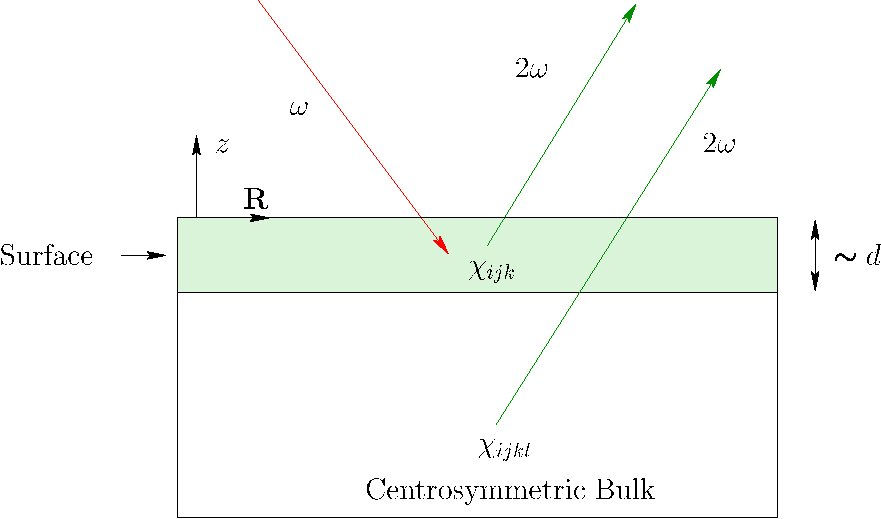
\includegraphics[scale=0.6]{images/system}
\caption{(Color Online) Sketch of the semi-infinite system with a 
centrosymmetric bulk. The surface region is of width $\sim d$. 
The incoming photon of frequency $\go$ is represented by
a downward red arrow, whereas both the surface and bulk created second
harmonic photons of frequency $2\go$ are represented by upward
green arrows. The red color suggests an incoming infrared photon with
a green second harmonic photon. The dipolar ($\chi_{\rma\rmb\rmc}$), and 
quadrupolar ($\chi_{\rma\rmb\rmc\rml}$) susceptibility tensors are shown 
in the regions where they are different from zero. The axis has $z$
perpendicular to the surface and $\mbf{R}$ parallel to it.\label{fsystem}}
\end{figure}

If we move to the surface of the semi-infinite system our assumption 
of centrosymmetry breaks down, and there is no restriction in 
$\chi_{\rma\rmb\rmc}$. We conclude that the leading term
of the polarization in a surface region is given by
\begin{align}\label{sshgp1}
\int dz 
P_{\rma}(\mbf{R},z)
\approx dP_{\rma}
\equiv
P_{\rma}^S
\equiv
\chi^S_{\rma\rmb\rmc}E_{\rmb}E_{\rmc},
\end{align}
where
% $\mbf{R}$ is a vector parallel to the surface which is
% perpendicular to $z$, $\cals$ is the surface area of the unit
% cell that characterizes the surface of the system, and 
$d$ is the
surface region from which the dipolar signal of $\bfP$ is
different from zero (see Fig.~\ref{fsystem}), and
$\mbf{P}^S\equiv d\mbf{P}$
 is the surface SH polarization. Then, from Eq.~\eqref{mshg} we obtain that
\begin{align}\label{sshgp2}
\chi_{\rma\rmb\rmc}^S=d\chi_{\rma\rmb\rmc}
\end{align}
is the
SH surface susceptibility. 
On the other hand, 
\begin{equation}\label{sshgp3}
P^b_{\rma}(\mbf{r})=\chi_{\rma\rmb\rmc\rml}E_{\rmb}(\mbf{r})\nabla_{\rmc}
E_{\rml}(\mbf{r}),  
\end{equation}
gives the bulk polarization. We immediately recognize that the surface
polarization is of dipolar order while the bulk polarization is of
quadrupolar order. The surface, $\chi^S_{\rma\rmb\rmc}$, and bulk, 
$\chi_{\rma\rmb\rmc\rml}$, susceptibility tensor ranks are three and 
four, respectively. We will only concentrate on surface SHG in this article 
even though bulk generated SH is also a very important optical phenomenon. 
Also, we leave out of this article other interesting surface SH phenomena like, electric field
induced second harmonic (EFISH), which would be represented by a
surface susceptibility  tensor of quadrupolar origin.
In centrosymmetric systems for which the quadrupolar bulk
response is much smaller than the dipolar surface response, SH is
readily used as a very useful and powerful 
optical surface probe.\cite{downer_optical_2001}

In the following sections we present the theoretical approach to
derive
the expressions for the 
surface susceptibility tensor $\chi^S_{\rma\rmb\rmc}$.

\section{Length Gauge}\label{longi}

We follow the article by Aversa and Sipe\cite{aversaPRB95} to calculate 
the optical properties of a given system within the longitudinal gauge. 
More recent derivations
can also be found in Refs. \onlinecite{sipe_second-order_2000,lambrechtPSSB00}.  
Assuming the long-wavelength approximation which implies 
a position independent electric field, 
$\bfE(t)$,  
the Hamiltonian in the length gauge approximation is given by
\begin{equation}\label{ache}
\hat{H}=\hat{H}^\gs_0-e \hat\bfr \cdot \bfE,
\end{equation}
with
\begin{align}\label{ache.1}
\hat H^\gs_0=\hat H^\lda_0
 + \cals(\bfr,\bfp)
,
\end{align} 
as the unperturbed Hamiltonian.
The LDA Hamiltonian can be expressed as follows,
\begin{align}\label{ache.2}
\hat H^\lda_0&=\frac{\hat p^2}{2m_e}  + \hat V^\ps
\nonumber\\
\hat V^\ps
&=\hat V^l(\hat\bfr) + \hat V^\nl
,
\end{align}  
where $\hat V^l(\hat\bfr)$ and $\hat V^\nl$ are the local and
the non-local parts of the  
crystal 
pseudopotential $\hat V^\ps$. For the latter, we have that
\begin{align}\label{ache.3n}
 V^\nl(\bfr,\bfr')
\equiv \bra{\bfr}\hat V^\nl\ket{\bfr'}\neq 0 \quad\mathrm{for}\quad\bfr\neq\bfr'
,
\end{align}
where $V^\nl(\bfr,\bfr')$ is a function of $\bfr$ and $\bfr'$
representing the non-local contribution of the pseudopotential.
The Schr\"odinger equation reads
\begin{align}\label{ache.4} 
\left(
\frac{-\hbar^2}{2m_e}\nabla^2
 + \hat V^l(\bfr)\right)\psi_{n\bfk}(\bfr)
 + \int d\bfr'\hat V^\nl(\bfr,\bfr')\psi_{n\bfk}(\bfr')
=E_i\psi_{n\bfk}(\bfr)
,
\end{align} 
where
%$\psi_{n\bfk}(\bfr)=\braket{\bfr}{n\bfk}=\sqrt{\gO/8\pi^3}e^{i\bfk\cdot\bfr}u_{n\bfk}(\bfr)$,
$\psi_{n\bfk}(\bfr)=\braket{\bfr}{n\bfk}=e^{i\bfk\cdot\bfr}u_{n\bfk}(\bfr)$,
are the real space representations of the Bloch states $\ket{n\bfk}$ labelled
by the band index $n$ and the crystal momentum $\bfk$, and $u_{n\bfk}(\bfr)$
is cell periodic. $m_e$ is the bare mass of the electron and $\gO$ is the 
unit cell volume. The nonlocal scissors operator is given by 
\begin{equation}\label{chon.0}
\cals(\bfr,\bfp)=\hbar\gS\sum_n\int d^3k'(1-f_n(\bfk)) \ket{n\bfk'}\bra{n\bfk'}
,
\end{equation}
where $f_n(\bfk)$ is the occupation number, that for $T=0$ K, is
independent of $\bfk$, and is one for filled bands and zero for
unoccupied bands. For semiconductors the filled bands correspond to
valence
bands  ($n=v$) and the unoccupied bands to conduction bands
 ($n=c$). 
We have that
\begin{align}\label{chon.1}  
H^\lda_0\ket{n\bfk}&=\hbar\go^\lda_n(\bfk)\ket{n\bfk}
\nonumber\\
H^\gs_0\ket{n\bfk}&=\hbar\go^\gs_n(\bfk)\ket{n\bfk}
,
\end{align} 
where 
\begin{align}\label{chon.78}
\hbar\go^\gs_n(\bfk)=\hbar\go^\lda_n(\bfk)+\hbar\gS(1-f_n)
,
\end{align}
is the
 scissored
energy. Here, 
$\hbar\gS$ is the value by which the conduction bands are rigidly
($\bfk$-independent)
 shifted
upwards in energy, also known as the scissors shift. $\gS$ could be taken to be
$\bfk$ dependent, but for most calculations (like the ones presented
here), a rigid shift is sufficient. We can take 
$\hbar\gS=E_g-E_g^\lda$ where $E_g$ could be the experimental band gap 
or GW band gap taken at the $\Gamma$ point, i.e. $\bfk=0$.
We used the fact that 
$\ket{n\bfk}^\lda\approx\ket{n\bfk}^\gs$, thus negating the need to label
the Bloch states with the LDA or $\gs$ superscripts. 
The matrix elements of $\bfr$ are split between the {\it intraband} 
($\bfr_i$) and {\it interband} ($\bfr_e$) parts , where 
$\bfr=\bfr_i+\bfr_e$ and\cite{adamsJCP53,blountSSP62,aversaPRB95}
\begin{align}\label{rnminn}
\bra{n\bfk}\hat\bfr_i\ket{m\bfk'} &= \gd_{nm}\left[\gd(\bfk-\bfk')\bfgxi_{nn}(\bfk)
+i\nabla_\bfk\gd(\bfk-\bfk')\right], \\
\bra{n\bfk}\hat\bfr_e\ket{m\bfk'} &=
(1-\gd_{nm})\gd(\bfk-\bfk')\bfgxi_{nm}(\bfk)
,
\label{rnmenn}
\end{align}
and
\begin{equation}\label{zetann}
\bfgxi_{nm}(\bfk) \equiv i\frac{(2\pi)^3}{\gO}\int_{\gO} d\bfr\, u^*_{n\bfk}(\bfr)\nabla_{\bfk}u_{m\bfk}(\bfr).
\end{equation}
The interband part $\bfr_e$ can
be obtained as follows. 
We start by introducing the 
velocity operator
\begin{align}\label{vop}
\hat\bfv^\gs&=
\frac{1}{i\hbar}[\hat\bfr,\hat{H}^\gs_0]
,
\end{align}
and calculating its matrix elements
\begin{equation}\label{conhrnm}
i\hbar\bra{n\bfk}
\bfv^\gs
\ket{m\bfk}
=
\bra{n\bfk}
[\hat\bfr,\hat{H}^\gs_0]
\ket{m\bfk}
=\bra{n\bfk}\hat\bfr\hat{H}^\gs_0-\hat{H}^\gs_0\hat\bfr\ket{m\bfk}
=(\hbar\go^\gs_m(\bfk)-\hbar\go^\gs_n(\bfk))\bra{n\bfk}\hat\bfr\ket{m\bfk}
,
\end{equation}
thus defining $\go^\gs_{nm}(\bfk)=\go^\gs_n(\bfk)-\go^\gs_m(\bfk)$ we get
\begin{align}\label{pmnrmn}
\bfr_{nm}(\bfk)
&=
\frac{\bfv^\gs_{nm}(\bfk)}{i\go^\gs_{nm}(\bfk)}
\quad\quad n\notin D_m
,
\end{align} 
which can be identified as 
$\bfr_{nm}=(1-\gd_{nm})\bfgxi_{nm}\to \bfr_{e,nm}$.
Here, $D_m$ are all the possible degenerate $m$-states.
When $\bfr_i$ appears in
commutators we use\cite{aversaPRB95} 
\begin{equation}\label{conmri3n}
\bra{n\bfk}[\hat\bfr_i,\hat\calo]\ket{m\bfk'}
=i\gd(\bfk-\bfk')(\calo_{nm})_{;\bfk}
,
\end{equation}  
with
\begin{equation}\label{gendevnn}
(\calo_{nm})_{;\bfk}=
\nabla_\bfk
\calo_{n m}(\bfk)
- 
i
\calo_{nm}(\bfk)
\left(
\bfgxi_{nn}(\bfk)
-
\bfgxi_{mm}(\bfk)
\right)
,
\end{equation} 
where ``$;\bfk$'' denotes the generalized derivative (see Appendix \ref{reri}). 

As can be seen from Eq.~\eqref{ache.1} and \eqref{ache.2},
both $\hat S$ and $\hat V^\nl$ are nonlocal potentials. Their contribution 
in the calculation of the optical response has to be taken in order to
get reliable results.\cite{ismailPRL01}
We proceed as follows; from Eqs.~\eqref{vop}, \eqref{ache.1} and
\eqref{ache.2}
 we find
\begin{align}\label{vop2}
\hat\bfv^\gs&=
\frac{\hat\bfp}{m_e}
+
\frac{1}{i\hbar}[\hat\bfr,\hat V^\nl(\bfr,\bfr')]
+
\frac{1}{i\hbar}[\hat\bfr,\hat\cals(\bfr,\bfp)]
\nonumber\\
&\equiv
\hat\bfv
+
\hat\bfv^\nl
+\hat\bfv^\cals
=
\hat\bfv^\lda
+\hat\bfv^\cals
,
\end{align}
where we have defined
\begin{align}\label{conhr}
\hat\bfv
&=\frac{\hat\bfp}{m_e}
\nonumber\\
\hat\bfv^\nl
&=
\frac{1}{i\hbar}[\hat\bfr,\hat V^\nl]
\nonumber\\
\hat\bfv^\cals
&=
\frac{1}{i\hbar}[\hat\bfr,\hat S(\bfr,\bfp)]
\nonumber\\
\hat\bfv^\lda
&=
\hat\bfv
+\hat\bfv^\nl
\end{align}  
with $\hat\bfp=-i\hbar\bfgnabla$ the momentum operator.
Using Eq.~\eqref{chon.0}, we obtain that the
matrix elements of $\hat\bfv^\cals$ are given by
\begin{equation}\label{chon.2} 
\bfv^\cals_{nm}=i\gS f_{mn}\bfr_{nm},
%=\frac{\gS f_{mn}}{\go^\lda_{nm}}\bfv^\lda_{nm}
\end{equation}
with $f_{nm}=f_n-f_m$,
where we see that $\bfv^\cals_{nn}=0$, then
\begin{align}\label{chon.8}
\bfv^\gs_{nm}
&=
\bfv^\lda_{nm}+i\gS f_{mn}\bfr_{nm}
\nonumber\\
&=
\bfv^\lda_{nm}+i\gS f_{mn}\frac{\bfv^\gs_{nm}(\bfk)}{i\go^\gs_{nm}(\bfk)}
\nonumber\\
\bfv^\gs_{nm}
\frac{\go^\gs_{nm}-\gS f_{mn}}{\go^\gs_{nm}}
&=
\bfv^\lda_{nm}
\nonumber\\
\bfv^\gs_{nm}
\frac{\go^\lda_{nm}}{\go^\gs_{nm}}
&=
\bfv^\lda_{nm}
\nonumber\\
\frac{\bfv^\gs_{nm}}{\go^\gs_{nm}}
&=
\frac{\bfv^\lda_{nm}}{\go^\lda_{nm}}
,
\end{align}
since
$\go^\gs_{nm}-\gS f_{mn}=\go^\lda_{nm}$. Therefore, 
\begin{align}\label{chon.9}
\bfv^\gs_{nm}(\bfk)
&=
\frac{\go^\gs_{nm}}{\go^\lda_{nm}}\bfv^\lda_{nm}(\bfk)
=\left(1+\frac{\gS}{\go_c(\bfk)-\go_v(\bfk)}\right)\bfv^\lda_{nm}(\bfk)
\quad\quad n\notin D_m
\nonumber\\
\bfv^\gs_{nn}(\bfk)
&=
\bfv^\lda_{nn}(\bfk)
,
\end{align} 
and Eq.~\eqref{pmnrmn} gives
\begin{align}\label{chon.10}
\bfr_{nm}(\bfk)
=
\frac{\bfv^\gs_{nm}(\bfk)}{i\go^\gs_{nm}(\bfk)}
=
\frac{\bfv^\lda_{nm}(\bfk)}{i\go^\lda_{nm}(\bfk)}
\quad\quad n\notin D_m
.
\end{align}
The matrix elements
of $\bfr_e$ are the same whether we use the LDA or the scissored
Hamiltonian and there is no need to label them with either LDA
or S superscripts. Thus,
we can write
\begin{equation}\label{chon.98}
\bfr_{e,nm}\to
\bfr_{nm}(\bfk)=\frac{\bfv^\lda_{nm}(\bfk)}{i\go^\lda_{nm}(\bfk)}
\quad\quad n\notin D_m
,
\end{equation}   
which gives the interband matrix elements of the position operator
in terms of the matrix elements of $\hat\bfv^\lda$. 
These matrix elements include the matrix elements of
$\bfv^\nl_{nm}(\bfk)$ which can be readily calculated\cite{francesco} for 
fully separable nonlocal pseudopotentials in the 
Kleinman-Bylander 
form.\cite{mottaCMS10,kleinman_efficacious_1982,adolphPRB96}
In Appendix \ref{appvnl} we outline how this  
can be accomplished. 

\section{Time-dependent Perturbation Theory}\label{tdpt}

In the independent particle approximation, we use the electron density
operator $\hat\gr$ to obtain the expectation value of any observable
$\calo$ as
\begin{equation}\label{traza}
\calo=\mathrm{Tr}(\hat\calo\hat\rho)=\mathrm{Tr}(\hat\rho\hat\calo),
\end{equation}
where $\mathrm{Tr}$ is the trace and is invariant under cyclic permutations.
The dynamic equation of motion for $\gr$ is given by
\begin{equation}\label{eqrho}
i\hbar \frac{d\hat\gr}{dt}=[\hat{H},\hat\gr]
,
\end{equation}
where it is more convenient to work in the interaction picture. We transform 
all operators according to 
\begin{equation}\label{ip}
\hat{\calo}_I=\hat{U}\hat{\calo}\hat{U}^\dagger,
\end{equation}
where
\begin{equation}\label{ou}
\hat{U}=e^{i\hat{H}_0t/\hbar},
\end{equation}
is the unitary operator that shifts us to the interaction picture.
Note that $\hat\calo_I$ depends on time even if $\hat\calo$ does not.
Then, we transform Eq.~\eqref{eqrho} into
\begin{equation}\label{intrho}
i\hbar\frac{d\hat\gr_I(t)}{dt}=[-e\hat\bfr_I(t)\cdot\bfE(t),\hat\gr_I(t)],
\end{equation}
that leads to
\begin{equation}\label{intrho2}
\hat\gr_I(t)=\hat\gr_I(t=-\infty)
+
\frac{ie}{\hbar}\int_{-\infty}^t dt'[\hat\bfr_I(t')\cdot\bfE(t'),\hat\gr_I(t')].
\end{equation}
We assume that the interaction is switched-on adiabatically and
choose a time-periodic perturbing field, to write
\begin{equation}\label{efield}
\bfE(t)=\bfE e^{-i\go t}e^{\eta t}=\bfE e^{-i\got t}
,
\end{equation}
with
\begin{equation}\label{got}
\got=\go+i\eta
,
\end{equation} 
where $\eta > 0$ assures
that at $t=-\infty$ the interaction is zero and has its full strength $\bfE$ 
at $t=0$. After computing the required time integrals one takes
$\eta\to 0$. 
Also, $\hat\gr_I(t=-\infty)$ should be time independent and thus 
$[\hat{H},\hat\rho]_{t=-\infty}=0$, This implies that 
$\hat\gr_I(t=-\infty)=\hat\rho(t=-\infty)\equiv\hat\rho_0$,
where $\hat\rho_0$ is
the density matrix of the unperturbed ground state,
such that
\begin{equation}\label{nrhon}
\bra{n\bfk}\hat\gr_0\ket{m\bfk'}=f_n(\hbar\go^\gs_n(\bfk))\gd_{nm}\gd(\bfk-\bfk')
,
\end{equation}
with $f_n(\hbar\go^\gs_n(\bfk))=f_{n\bfk}$ as the Fermi-Dirac distribution function.

We solve Eq.~\eqref{intrho2} using the standard iterative
solution, for which we write
\begin{equation}\label{rhop}
\hat\rho_I=\hat\rho_I^{(0)}+\hat\rho_I^{(1)}+\hat\rho_I^{(2)}+\cdots
,
\end{equation}
where $\hat\rho_I^{(N)}$ is the density operator to order $N$ in $\bfE(t)$.
Then, Eq.~\eqref{intrho2} reads
\begin{equation}\label{intrho3}
\hat\rho_I^{(0)}+\hat\rho_I^{(1)}+\hat\rho_I^{(2)}+\cdots
=\hat\gr_0
+
\frac{ie}{\hbar}\int_{-\infty}^t dt'[\hat\bfr_I(t')\cdot\bfE(t'),
\hat\rho_I^{(0)}+\hat\rho_I^{(1)}+\hat\rho_I^{(2)}+\cdots
]
,
\end{equation}
where, by equating equal orders in the perturbation, we find
\begin{equation}\label{rho0}
\hat\gr_I^{(0)}\equiv\hat\gr_0
,
\end{equation}
and
\begin{equation}\label{rhoN}
\hat\gr_I^{(N)}(t)=
\frac{ie}{\hbar}
\int_{-\infty}^t dt'[\hat\bfr_I(t')\cdot\bfE(t'),\hat\gr^{(N-1)}_I(t')].
\end{equation}
It is simple to show that matrix elements of Eq. (\ref{rhoN}) satisfy
$\bra{n\bfk}\gr_I^{(N+1)}(t)\ket{m\bfk'}=\gr^{(N+1)}_{I,nm}(\bfk)\gd(\bfk-\bfk')$,
with
\begin{equation}\label{rtilde}
\gr^{(N+1)}_{I,nm}(\bfk;t)
=\frac{ie}{\hbar}\int_{-\infty}^t dt'
\bra{n\bfk}
[\hat\bfr_I(t'),\hat\gr^{(N)}_I(t')]
\ket{m\bfk}
\cdot\bfE(t')
.
\end{equation}

We now work out the commutator of Eq.~\eqref{rtilde}. Then,
\begin{align}\label{conmu1}
\bra{n\bfk}
[\hat\bfr_I(t),\hat\gr^{(N)}_I(t)]
\ket{m\bfk}
&=
\bra{n\bfk}
[\hat{U}\hat\bfr\hat{U}^\dagger,\hat{U}\hat\gr^{(N)}(t)\hat{U}^\dagger]
\ket{m\bfk}
\nonumber \\
&=
\bra{n\bfk}
\hat{U}[\hat\bfr,\hat\gr^{(N)}(t)]\hat{U}^\dagger
\ket{m\bfk}
\\
&=
e^{i\go^\gs_{nm\bfk}t}
\left(
\bra{n\bfk}
[\hat\bfr_e,\hat\gr^{(N)}(t)]
+
[\hat\bfr_i,\hat\gr^{(N)}(t)]
\ket{m\bfk}
\right)
\nonumber
.
\end{align}
% where the time dependence of operator's interaction picture is
% explicitly shown by the exponential factor, and the implicit
% dependence of $\hat\rho^{(N)}$ inherited from Eq.~\eqref{eqrho} is
% shown by its $t$ argument.
We calculate the interband term first, so using Eq.~\eqref{chon.98} we obtain
\begin{align}\label{conmu2}
\bra{n\bfk}
[\hat\bfr_e,\hat\gr^{(N)}(t)]
\ket{m\bfk}
&=
\sum_{\ell}
\left(
\bra{n\bfk}
\hat\bfr_e
\ket{\ell\bfk}
\bra{\ell\bfk}
\hat\gr^{(N)}(t)
\ket{m\bfk}
\right.
\nonumber \\
&
\left.
-
\bra{n\bfk}
\hat\gr^{(N)}(t)
\ket{\ell\bfk}
\bra{\ell\bfk}
\hat\bfr_e
\ket{m\bfk}
\right)
\nonumber \\
&=
\sum_{\ell\ne n,m}
\left(
\bfr_{n\ell}(\bfk)
\gr^{(N)}_{\ell m}(\bfk;t)
-
\gr^{(N)}_{n\ell}(\bfk;t)
\bfr_{\ell m}(\bfk)
\right)
\nonumber\\
&\equiv
\bfR^{(N)}_e(\bfk;t)
,
\end{align}

and from Eq.~\eqref{conmri3n},
\begin{equation}\label{conmri4}
\bra{n\bfk}[\hat\bfr_i,\hat\rho^{(N)}(t)]\ket{m\bfk'}
=i \gd(\bfk-\bfk') (\rho^{(N)}_{nm}(t))_{;\bfk}
\equiv \gd(\bfk-\bfk')\bfR_i^{(N)}(\bfk;t)
.
\end{equation}
Then Eq.~\eqref{rtilde} becomes
\begin{equation}\label{rtilde2}
\gr^{(N+1)}_{I,nm}(\bfk;t)
=\frac{ie}{\hbar}\int_{-\infty}^t dt'
e^{i(\go^\gs_{nm\bfk}-\got)t'}
\left[R_e^{\rmb(N)}(\bfk;t')+R_i^{\rmb(N)}(\bfk;t')\right]E^{\rmb}
,
\end{equation}
where the roman superindices
$\rma,\rmb,\rmc$ denote Cartesian components that are summed over if repeated.
Starting from the linear response and proceeding from Eq.~\eqref{nrhon} and ~\eqref{conmu2},
\begin{align}\label{R0e}
R_e^{\rmb(0)}(\bfk;t)
&=
\sum_{\ell}
\left(
r^{\rmb}_{n\ell}(\bfk)
\gr^{(0)}_{\ell m}(\bfk)
-
\gr^{(0)}_{n\ell}(\bfk)
r^{\rmb}_{\ell m}(\bfk)
\right)
\nonumber \\
&=
\sum_{\ell}
\left(
r^{\rmb}_{n\ell}(\bfk)
\gd_{\ell m}f_m(\hbar\go^\gs_m(\bfk))
-
\gd_{n\ell}f_n(\hbar\go^\gs_n(\bfk))
r^{\rmb}_{\ell m}(\bfk)
\right)
\nonumber \\
&=
f_{mn\bfk}
r^{\rmb}_{nm}(\bfk)
,
\end{align}
where $f_{mn\bfk}=f_{m\bfk}-f_{n\bfk}$.
From now on,
it should be clear that the matrix elements of $\bfr_{nm}$ imply
$n\notin D_m$.
We also have from Eq.~\eqref{conmri4} and Eq.~\eqref{gendevnn} that
\begin{equation}\label{R0i}
R_i^{\rmb(0)}(\bfk)=i(\rho^{(0)}_{nm})_{;k^{\rmb}}=i\gd_{nm}(f_{n\bfk})_{;k^{\rmb}}=i\gd_{nm}\nabla_{k^{\rmb}} f_{n\bfk}
.
\end{equation}
For a semiconductor at $T=0$, $f_{n\bfk}$ is one if the state
$\ket{n\bfk}$ is a valence state and zero if it is a conduction state; 
thus $\nabla_\bfk f_{n\bfk}=0$ and $\bfR_i^{(0)}=0$ and
the linear response has no contribution from
intraband transitions.
 Then,
\begin{align}\label{rtilde2n}
\gr^{(1)}_{I,nm}(\bfk;t)
&=\frac{ie}{\hbar}
f_{mn\bfk}
r^{\rmb}_{nm}(\bfk)E^{\rmb}
\int_{-\infty}^t dt'
e^{i(\go^\gs_{nm\bfk}-\got)t'}
\nonumber \\
&=\frac{e}{\hbar}
f_{mn\bfk}
r^{\rmb}_{nm}(\bfk)E^{\rmb}
\frac{e^{i(\go^\gs_{nm\bfk}-\got)t}}
{\go^\gs_{nm\bfk}-\got}
\nonumber \\
&=
e^{i\go^\gs_{nm\bfk}t}
B^{\rmb}_{mn}(\bfk)E^{\rmb}(t)
\nonumber \\
&=
e^{i\go^\gs_{nm\bfk}t}
\rho^{(1)}_{nm}(\bfk;t)
,
\end{align}
with
\begin{equation}\label{rho1} 
B^{\rmb}_{nm}(\bfk,\go)=
\frac{e}{\hbar}\frac{f_{mn\bfk}r^{\rmb}_{nm}(\bfk)}{\go^\gs_{nm\bfk}-\got}
,
\end{equation} 
and
\begin{equation}\label{rhonoi1}
\rho^{(1)}_{nm}(\bfk;t)=B^{\rmb}_{mn}(\bfk,\go)E^{\rmb}(\go)e^{-i\got t}
.
\end{equation}

Now, we calculate the second-order response. Then, from Eq.~\eqref{conmu2}
\begin{align}\label{R1e}
R_e^{\rmb(1)}(\bfk;t)
&=
\sum_{\ell}
\left(
r^{\rmb}_{n\ell}(\bfk)
\gr^{(1)}_{\ell m}(\bfk;t)
-
\gr^{(1)}_{n\ell}(\bfk;t)
r^{\rmb}_{\ell m}(\bfk)
\right)
\nonumber \\
&=
\sum_{\ell}
\left(
r^{\rmb}_{n\ell}(\bfk)
B^{\rmc}_{\ell m}(\bfk,\go)
-
B^{\rmc}_{n\ell}(\bfk,\go)
r^{\rmb}_{\ell m}(\bfk)
\right)E^{\rmc}(t)
,
\end{align}
and from Eq.~\eqref{conmri4}
\begin{equation}\label{R1i}
R_i^{\rmb(1)}(\bfk;t)=
i(\rho^{(1)}_{nm}(t))_{;k^{\rmb}}=
iE^{\rmc}(t)(B^{\rmc}_{nm}(\bfk,\go))_{;k^{\rmb}}
.
\end{equation}

Using Eqs.~\eqref{R1e} and ~\eqref{R1i} in Eq. (\ref{rtilde2}),
we obtain
\begin{align}\label{rtilde33}
\gr^{(2)}_{I,nm}(\bfk;t)
&=
\frac{ie}{\hbar}
\bigg[
\sum_{\ell}
\Big(
r^{\rmb}_{n\ell}(\bfk)
B^{\rmc}_{\ell m}(\bfk,\go)
-
B^{\rmc}_{n\ell}(\bfk,\go)
r^{\rmb}_{\ell m}(\bfk)
\Big)
\nonumber \\
&+
i
(B^{\rmc}_{nm}(\bfk,\go))_{;k^{\rmb}}
\bigg]
E^{\rmb}_{\go}E_{\go}^{\rmc}
\int_{-\infty}^t dt'
e^{i(\go^\gs_{nm\bfk}-2\got)t'}
\nonumber \\
&=
\frac{e}{\hbar}
\bigg[
\sum_{\ell}
\Big(
r^{\rmb}_{n\ell}(\bfk)
B^{\rmc}_{\ell m}(\bfk,\go)
-
B^{\rmc}_{n\ell}(\bfk,\go)
r^{\rmb}_{\ell m}(\bfk)
\Big)
\nonumber \\
&+
i
(B^{\rmc}_{nm}(\bfk,\go))_{;k^{\rmb}}
\bigg]
E^{\rmb}_{\go}E_{\go}^{\rmc}
\frac{e^{i(\go^\gs_{nm\bfk}-2\got)t}}
{\go^\gs_{nm\bfk}-2\got}
\nonumber \\
&=
e^{i\go^\gs_{nm\bfk}t}
\rho_{nm}^{(2)}(\bfk;t)
.
\end{align}
Now, we write
$\rho_{nm}^{(2)}(\bfk;t)=\rho_{nm}^{(2)}(\bfk;2\go)e^{-i2\got t}$,
with
\begin{align}\label{rho2}
\gr_{nm}^{(2)}(\bfk;2\go)&=\frac{e}{i\hbar}\frac{1}{\go^\gs_{nm\bfk}-2\got}
\bigg[-(B_{nm}^{\rmc}(\bfk,\go)_{;k^{\rmb}}
\nonumber \\
&
+i\sum_\ell\Big(r_{n\ell}^{\rmb}B_{\ell m}^{\rmc}(\bfk,\go) - B_{n\ell}^{\rmc}(\bfk,\go)
  r_{\ell m}^{\rmb}\Big)
\bigg] 
E^{\rmb}(\go)E^{\rmc}(\go)
\end{align} 
where 
$B_{\ell m}^{\rma}(\bfk,\go)$ are given by Eq.~\eqref{rho1}. 
We remark that $\bfr_{nm}(\bfk)$  are
the same whether calculated with the LDA or the scissored Hamiltonian. 
We chose the former in this article.

\section{Layered Current Density}\label{cd}

In this section, we derive the expressions for the microscopic current
density of a given layer in the unit cell of the system.
The approach we use to study the surface of a semi-infinite
semiconductor crystal is as follows. Instead of using a
semi-infinite system, we replace it by a slab (see Fig.~\ref{fslab}).
The slab consists of a front and back surface, and in between these
two surfaces is the bulk of the system. 
In general the surface of a crystal reconstructs or relaxes as the atoms
move to find equilibrium positions. This is due to the fact that
the otherwise
balanced forces are disrupted when the surface atoms do not find their 
partner atoms that are now absent at the surface of the slab. 

To take the reconstruction or relaxation into account, we take ``surface'' to mean
the true surface of the first layer of atoms, and
some of the atomic sub-layers adjacent to it.
Since the front and the back
surfaces of the slab are usually identical the total slab is
centrosymmetric. This implies that 
$\chi^{\mathrm{slab}}_{\rma\rmb\rmc}=0$, and thus we must
find a way to bypass this characteristic of a centrosymmetric slab 
in order to have a finite $\chi^s_{\rma\rmb\rmc}$ representative of the
surface. Even if the front and back surfaces of the slab 
are different, breaking the centrosymmetry and therefore giving an
overall $\chi^{\mathrm{slab}}_{\rma\rmb\rmc}\ne 0$, we still
need a procedure to extract the front surface $\chi^f_{\rma\rmb\rmc}$
and the back surface $\chi^b_{\rma\rmb\rmc}$ from the non-linear
susceptibility 
$\chi^{\mathrm{slab}}_{\rma\rmb\rmc}=\chi^f_{\rma\rmb\rmc}-\chi^b_{\rma\rmb\rmc}$
 of the entire slab.

A convenient way to accomplish the separation of the SH signal of
either surface is to introduce a ``cut function'', $\calc(z)$, which is 
usually taken to be unity over one half of the slab and zero over 
the other half.\cite{reining_microscopic_1994}
 In this case $\calc(z)$ will give the contribution of the 
side of the slab for which $\calc(z)=1$. We can generalize this 
simple choice for $\calc(z)$ by a top-hat cut function
$\calc^\ell(z)$ that selects a given layer,
\begin{equation}
\label{sz}
\calc^\ell(z)=\Theta(z-z_\ell+\Delta_\ell^{\rmb})
            \Theta(z_\ell-z+\Delta_\ell^f),
\end{equation}
where $\Theta$ is the Heaviside function. Here, $\Delta_\ell^{f/b}$
is the distance that the $\ell$-th layer extends towards the front
$(f)$ or back $(b)$ from its $z_\ell$ position. 
$\Delta_\ell^f+\Delta_\ell^b$ is the thickness of layer $\ell$ 
(see Fig.~\ref{fslab}).
\begin{figure}[b]
\centering
%\includegraphics[height=5cm,width=7cm]{slab}
\includegraphics[scale=.7]{images/slab}
\caption{A sketch of a slab where the circles represent atoms.\label{fslab}}
\end{figure}

Now, we show how this ``cut function'' $\calc^\ell(z)$ is introduced in
the calculation of $\chi_{\rma\rmb\rmc}$. 
The microscopic current density is given by
\begin{equation}\label{jmic}
\bfj(\bfr,t)=\mathrm{Tr}(\hat\bfj(\bfr)\hat\rho(t)),
\end{equation}
where the operator for the electron's current is
\begin{equation}\label{hatjmic}
\hat\bfj(\bfr)=\frac{e}{2}\left(\hat\bfv^\gs\ket{\bfr}\bra{\bfr}
+\ket{\bfr}\bra{\bfr}\hat\bfv^\gs\right), 
\end{equation}
where $\hat{\mbf{v}}^\gs$ is the electron's velocity operator to be dealt
with below. We define
$\hat\mu\equiv\ket{\bfr}\bra{\bfr}$ and use the cyclic invariance of
the trace to write
\begin{align}\label{jmic2}
\mathrm{Tr}(\hat\bfj(\bfr)\hat\rho(t)&=\mathrm{Tr}(\hat\rho(t)\hat\bfj(\bfr))=
\frac{e}{2}
\left(
\mathrm{Tr}(\hat\rho\hat\bfv^\gs\hat\mu)
+
\mathrm{Tr}(\hat\rho\hat\mu\hat\bfv^\gs)
\right)
\nonumber\\
&=
\frac{e}{2}
\sum_{n\bfk}
\left(
\bra{n\bfk}\hat\rho\hat\bfv^\gs\hat\mu\ket{n\bfk}
+
\bra{n\bfk}\hat\rho\hat\mu\hat\bfv^\gs\ket{n\bfk}
\right)
\nonumber\\
&=
\frac{e}{2}
\sum_{nm\bfk}
\bra{n\bfk}\hat\rho\ket{m\bfk}
\left(
\bra{m\bfk}\hat\bfv^\gs\ket{\bfr}\braket{\bfr}{n\bfk}
+
\braket{m\bfk}{\bfr}\bra{\bfr}\hat\bfv^\gs\ket{n\bfk}
\right)
\nonumber\\
\bfj(\bfr,t)&=
\sum_{nm\bfk}
\rho_{nm}(\bfk;t)\bfj_{mn}(\bfk;\bfr),
\end{align}
where
\begin{equation}\label{jmic3}
\bfj_{mn}(\bfk;\bfr)=
\frac{e}{2}
\left(
\bra{m\bfk}\hat\bfv^\gs\ket{\bfr}\braket{\bfr}{n\bfk}
+
\braket{m\bfk}{\bfr}\bra{\bfr}\hat\bfv^\gs\ket{n\bfk}
\right),
\end{equation}
are the matrix elements of the microscopic current operator,
and we have used the fact that the matrix elements between states $\ket{n\bfk}$
are diagonal in $\bfk$, i.e. proportional to $\gd(\bfk-\bfk')$.

Integrating the microscopic current $\mbf{j}(\mbf{r},t)$ over
the entire slab gives the averaged microscopic current density. 
If we want the contribution from only one region of the unit cell 
towards the total current, we can integrate $\mathbf{j}({\mathbf r},t)$ 
over the desired region. The contribution to the current density from the
$\ell$-th layer of the slab is given by
\begin{equation}\label{jsz}
\frac{1}{\Omega}\int d^3r\, \calc^\ell(z)\, \mathbf{j}(\mathbf{r},t)
 \equiv \mathbf{J}^{\ell}(t),
\end{equation}
where $\mathbf{J}^{\ell}(t)$ is the microscopic current in the
$\ell$-th layer.
Therefore we define
\begin{equation}\label{vcal}
e{\boldsymbol{\mathcal{V}}}^{\gs,\ell}_{mn}(\mathbf{k})
\equiv
%\frac{1}{\Omega}
\int d^3r\, \calc^\ell(z)\,\bfj_{mn}({\bfk};\bfr),
\end{equation}
to write
\begin{equation}\label{jmac}
J_a^{(N,\ell)}(t)=\frac{e}{\gO}
\sum_{mn\bfk}
\mathcal{V}^{\gs,a,\ell}_{mn}(\mathbf{k})
\rho^{(N)}_{nm}(\bfk;t),
\end{equation}
as the induced microscopic current of the $\ell$-th layer, to order $N$ 
in the external perturbation. The matrix elements of the 
density operator for $N=1,2$ are given by Eqs.~\eqref{rho1} and
\eqref{rho2} respectively. 
The Fourier component of microscopic current of Eq.~\eqref{jmac} is given by
\begin{equation}\label{jmac2}
J_{\rma}^{(N,\ell)}(\go_3)=\frac{e}{\gO}
\sum_{mn\bfk}
\calv^{\gs,\rma,\ell}_{mn}(\mathbf{k})
\rho^{(N)}_{nm}(\bfk;\go_3)
.
\end{equation}
We proceed to give an explicit expression of
$\calbv^{\gs,\ell}_{mn}(\mathbf{k})$.
From
Eqs.~\eqref{vcal} and \eqref{jmic3} we obtain
\begin{equation}\label{intj}
{\boldsymbol{\mathcal{V}}}^{\gs,\ell}_{mn}({\mathbf k})=
\frac{1}{2}
\int \mathrm{d}^3 r\,
 \calc^\ell(z)
\bigg[
\langle m\mathbf{k}|\mathbf{v}^\gs | \mathbf{r}\rangle
\langle \mathbf{r} | n \mathbf k \rangle +
\langle m\mathbf{k} | \mathbf{r}\rangle
\langle \mathbf{r} | \mathbf{v}^\gs | n \mathbf k \rangle\bigg]
,
\end{equation}  
and using the following property
\begin{equation}\label{nl.2}
\langle \mathbf{r} | \hat\bfv^\gs(\bfr,\bfr')| n\mathbf{k} \rangle
=\int d^3 r'' \bra{\mbf{r}}\hat\bfv^\gs(\bfr,\bfr')\ket{\mbf{r}''}
\braket{\mbf{r}''}{n\mbf{k}}
=\hat\bfv^\gs(\bfr,\bfr'')
\int d^3 r'' \braket{\mbf{r}}{\mbf{r}''}
\braket{\mbf{r}''}{n\mbf{k}}
=\hat\bfv^\gs(\bfr,\bfr')
\psi_{n\mathbf{k}}(\mathbf{r})
,
\end{equation}
that stems from the fact that the operator $\bfv^\gs(\bfr,\bfr')$ does not act on
$\bfr''$, we can write
\begin{align}\label{nl.3}
\calbv^{\gs,\ell}_{mn}({\mathbf k})
&=
\frac{1}{2}
\int \mathrm{d}^3 r\,
 \calc^\ell(z)
 \bigg[
\psi_{n\mathbf{k}}(\mathbf{r})
\hat\bfv^{\gs *}\psi^*_{m\mathbf{k}}(\mathbf{r})
+ 
\psi^*_{m\mathbf{k}}(\mathbf{r})\hat\bfv^\gs
\psi_{n\mathbf{k}}(\mathbf{r})
\bigg]
\nonumber\\
&=
\int \mathrm{d}^3 r\,
\psi^*_{m\mathbf{k}}(\mathbf{r})
\left[\frac{\calc^\ell(z) \bfv^\gs +
\bfv^\gs \calc^\ell(z)}{2}\right]
\psi_{n\mathbf{k}}(\mathbf{r})
\nonumber\\
&=
\int \mathrm{d}^3 r\,
\psi^*_{m\mathbf{k}}(\mathbf{r})
\calbv^{\gs,\ell}
\psi_{n\mathbf{k}}(\mathbf{r})
.
\end{align}
We used the hermitian property of $\bfv^\gs$ and defined
\begin{align}\label{nl.4}
\calbv^{\gs,\ell}
=
\frac{\calc^\ell(z) \bfv^\gs +
\bfv^\gs \calc^\ell(z)}{2}
,
\end{align} 
where the superscript $\ell$ is inherited from $\calc^\ell(z)$ and we
supress the dependance on $z$ from the increasingly crowded notation.  
We see that the replacement
\begin{align}\label{vcali}
\hat\bfv^\gs \to \hat\calbv^{\gs,\ell}=\left[\frac{\calc^\ell(z) \hat\bfv^\gs +
\hat\bfv^\gs \calc^\ell(z)}{2}\right]
,
\end{align} 
is all that is needed to change the
velocity operator of the electron $\hat\bfv^\gs$ to the new velocity
operator $\calbv^{\gs,\ell}$ that implicitly takes into account the
contribution of the region of the slab given by $\calc^\ell(z)$.
From Eq.~\eqref{vop2},
\begin{align}\label{vopii}
\calbv^{\gs,\ell}
&=
\calbv^{\lda,\ell}
+
\calbv^{\cals,\ell}
\nonumber\\
\calbv^{\lda,\ell}
&=
\calbv^{\ell}
+
\calbv^{\nl,\ell}
=
\frac{1}{m_e}
\calbp^{\ell}
+
\calbv^{\nl,\ell}
.
\end{align}
We remark that the simple relationship between 
$\bfv^{\sigma}_{nm}(\bfk)$ 
and 
$\bfv^{\lda}_{nm}(\bfk)$,
given in 
Eq.~\eqref{chon.9}, 
does not hold between
$\calbv^{\sigma,\ell}_{nm}(\bfk)$   
and 
$\calbv^{\lda,\ell}_{nm}(\bfk)$,
i.e.
$\calbv^{\sigma,\ell}_{nm}(\bfk)\ne
(\go^\gs_{nm}/\go_{nm})
\calbv^{\lda,\ell}_{nm}(\bfk)$ 
and
$\calbv^{\sigma,\ell}_{nn}(\bfk)\ne
\calbv^{\lda,\ell}_{nn}(\bfk)$
,
and thus, to calculate
$\calbv^{\sigma,\ell}_{nm}(\bfk)$ 
we must calculate the matrix elements of $\calbv^{\cals,\ell}$ and
$\calbv^{\lda,\ell}$ (separately)
according to the expressions of
Appendix \ref{calvs}.
% Using Eq.~\eqref{chon.9}, the matrix elements of Eq.~\eqref{vcali}
% are given by
% \begin{align}\label{end.1}
% \calbv^{\sigma,\ell}_{nm}(\bfk)
% &=
% \frac{1}{2}
% \sum_q
% \Big(
% \calc^\ell_{nq}\bfv^\sigma_{qm}
% +
% \bfv^\sigma_{nq}\calc^\ell_{qm}
% \Big)
% \nonumber\\
% &=
% \frac{1}{2}
% \Big(
% \calc^\ell_{nn}\bfv^\sigma_{nm}
% +
% \bfv^\sigma_{nn}\calc^\ell_{nm}
% +
% \calc^\ell_{nm}\bfv^\sigma_{mm}
% +
% \bfv^\sigma_{nm}\calc^\ell_{mm}
% \Big)
% \nonumber\\
% &+
% \frac{1}{2}
% \sum_{q\neq(nm)}
% \Big(
% \frac{\go^\sigma_{qm}}{\go_{qm}}
% \calc^\ell_{nq}\bfv^\lda_{qm}
% +
% \frac{\go^\sigma_{nq}}{\go_{nq}}
% \bfv^\lda_{nq}\calc^\ell_{qm}
% \Big)
% ,
% \end{align}
% \begin{align}\label{end.2}
% \calbv^{\sigma,\ell}_{nn}(\bfk)
% &=
% \frac{1}{2}
% \Big(
% \calc^\ell_{nn}\bfv^\sigma_{nn}
% +
% \bfv^\sigma_{nn}\calc^\ell_{nn}
% \Big)
% \nonumber\\
% &+
% \frac{1}{2}
% \sum_{q\neq n}
% \Big(
% \frac{\go^\sigma_{qn}}{\go_{qn}}
% \calc^\ell_{nq}\bfv^\lda_{qn}
% +
% \frac{\go^\sigma_{nq}}{\go_{nq}}
% \bfv^\lda_{nq}\calc^\ell_{qn}
% \Big)
% \nonumber\\
% &=
% \calc^\ell_{nn}\bfv^\lda_{nn}
% \nonumber\\
% &+
% \frac{1}{2}
% \sum_{q\neq n}
% \frac{\go^\sigma_{qn}}{\go_{qn}}
% \Big(
% \calc^\ell_{nq}\bfv^\lda_{qn}
% +
% \bfv^\lda_{nq}\calc^\ell_{qn}
% \Big)
% ,
% \end{align}

To limit the response to one surface, the equivalent of Eq.~\eqref{nl.4} 
for $\calbv^\ell=\calbp^\ell/m_e$ was proposed in 
Ref.~\onlinecite{reining_microscopic_1994} and later used in Refs.
\onlinecite{mendozaPRL98},
\onlinecite{mendoza_ab_2001},
\onlinecite{sanoPRB02},
 and \onlinecite{mejia_layer-by-layer_2004} 
also in the context of SHG. 
The layer-by-layer analysis of Refs. \onlinecite{hogan_optical_2003} 
and \onlinecite{castilloPRB03} used Eq.~\eqref{sz}, 
limiting the current response
to a particular layer of the slab and used to obtain the
anisotropic linear optical response of semiconductor surfaces.
However, the first formal derivation of this scheme is presented in
Ref.~\onlinecite{mendozaPRB06} for the linear response, and here in this 
article, for the second harmonic optical response of semiconductors.

%??d
% debemos mencionar que v caligrafica con tijeras esta mal calculada
% para la respuesta lineal y la inyeccion de corriente en el
% tratamiento capa por capa. Tambien, habria que ver que pasa con la
% inyeccion de espin capa-por-capa
%??u 


\section{Microscopic surface susceptibility}
In this section we obtain the expressions for the 
surface susceptibility tensor $\chi^S_{\rma\rmb\rmc}$.
We start with the basic relation $\bfJ=d\bfP/dt$ 
with $\bfJ$ the current calculated in Sec.~\ref{cd}. From Eq.~\eqref{jmac2} 
we obtain
\begin{equation}\label{Pjikn}
J_{\rma}^{(2,\ell)}(2\go)=-i2\got P_{\rma}(2\go)
=\frac{e}{\gO}
\sum_{mn\bfk}
\calv^{\gs,\rma,\ell}_{mn}(\mathbf{k})
\rho^{(2)}_{nm}(\bfk;2\go)
,
\end{equation}
and using Eqs.~\eqref{rho2} and \eqref{sshgp2} leads to
\begin{align}\label{Pjikn2}
\chi^{S,\ell}_{\rma\rmb\rmc}
&=
\frac{ie}{A E^{\rmb}_1E^{\rmc}_2 2\got}
\sum_{mn\bfk}
\calv^{\gs,\rma,\ell}_{mn}(\mathbf{k})
\rho^{(2)}_{nm}(\bfk;2\got)
\nonumber \\
&=
\frac{e^2}{A\hbar2\got}
\sum_{mn\bfk}
\frac{\calv^{\gs,\rma,\ell}_{mn}(\mathbf{k})}
{\go^\gs_{nm\bfk}-2\got}
\bigg[
-(B_{nm}^{\rmc}(\bfk,\go))_{;k^{\rmb}}
\nonumber \\
&
+i\sum_\ell\left(r_{n\ell}^{\rmb}B_{\ell m}^{\rmc}(\bfk,\go) -
  B_{n\ell}^{\rmc}(\bfk,\go) 
  r_{\ell m}^{\rmb}\right)
\bigg]
,
\end{align}
which gives the surface-like susceptibility of $\ell$-th layer, where 
$\calbv^\gs$ is given in Eq.~\eqref{vopii},
where $A=\gO/d$ is the surface area of the unit
cell that characterizes the surface of the system.
Using Eq.~\eqref{rho1} we
split this equation into
two contributions from the first and second terms on the right hand side,
\begin{equation}\label{chii}
\chi_{i,\rma\rmb\rmc}^{S,\ell}
=-\frac{e^3}{A\hbar^22\got}\sum_{mn\bfk}
\frac{\calv_{mn}^{\gs,\rma,\ell}}{\go^\gs_{nm}-2\got}
\left(\frac{f_{mn}r_{nm}^{\rmb}}{\go^\gs_{nm}-\got}\right)_{;k^{\rmc}},
\end{equation} 
and 
\begin{equation}\label{chie}
\chi_{e,\rma\rmb\rmc}^{S,\ell}
=\frac{ie^3}{A\hbar^22\got}\sum_{\ell mn\bfk}
\frac{\calv_{mn}^{\gs,\rma,\ell}}{\go^\gs_{nm}-2\got}
\left(
\frac{r_{n\ell}^{\rmc} r_{\ell m}^{\rmb} 
f_{m\ell}}{\go^\gs_{\ell m}-\got}
-\frac{r_{n\ell}^{\rmb} r_{\ell m}^{\rmc} 
f_{\ell n}}{\go^\gs_{n \ell}-\got}
\right),
\end{equation} 
where $\boldsymbol{\chi}^{S,\ell}_i$
 is related to intraband transitions and
$\boldsymbol{\chi}^{S,\ell}_e$
to interband transitions.
For the generalized derivative in Eq.~\eqref{chii} we use the chain rule 
\begin{equation}\label{gene2}
\left(\frac{f_{mn}r_{nm}^{\rmb}}{\go^\gs_{nm}-\got}\right)_{;k^{\rmc}}=
\frac{f_{mn}}{\go^\gs_{nm}-\got}\left(r_{nm}^\rmb\right)_{;k^{\rmc}}
-\frac{f_{mn}r_{nm}^{\rmb}\gD_{nm}^\rmc}{(\go^\gs_{nm}-\got)^2}
,
\end{equation}
and the following result
shown in Appendix \ref{gwk},
\begin{align}\label{eli.13}
\left(\go^\gs_{nm}\right)_{;k^{\rma}}
=
\left(\go^\lda_{nm}\right)_{;k^{\rma}}
= 
v_{nn}^{\lda,\rma}-v_{mm}^{\lda,\rma}\equiv\gD_{nm}^{\rma}
.
\end{align} 

In order to calculate the nonlinear susceptibility of any given layer 
$\ell$ we simply add the above terms $\boldsymbol{\chi}^{S,\ell}=
\boldsymbol{\chi}_e^{S,\ell}+\boldsymbol{\chi}_i^{S,\ell}$ and 
then calculate the surface susceptibility as 
\begin{equation}\label{chiijksur}
\bfgchi^S\equiv \sum_{\ell=1}^{N}\bfgchi^{S,\ell},
\end{equation} 
where $\ell=1$ is the first layer right at the surface, 
and $\ell=N$ is the bulk-like layer (at a distance $\sim d$ from the
surface  as seen in
Fig.~\ref{fsystem}), such that 
\begin{equation}\label{chiijksur2}
\bfgchi^{S,\ell=N}=0,
\end{equation}
in accordance to Eq.~\eqref{sshg} valid for a centrosymmetric environment. 
We note that the value of
$N$ is not universal.
This means that the slab needs to have enough atomic layers for 
Eq.~\eqref{chiijksur2} 
to be satisfied and to give converged results for $\bfgchi^S$. 
We can use Eq.~\eqref{chiijksur} for
either the front or the back surface.

We can see from the prefactors of Eqs. \eqref{chii} and \eqref{chie} 
that they diverge as $\got\to 0$. To remove this apparent divergence of 
$\bfgchi^{S,\ell}$, we perform a partial fraction expansion over $\got$. 
As shown in Appendix \ref{appv}, we use time-reversal invariance to 
remove these divergences and obtain the following expressions for $\bfgchi^S$,
\begin{equation}\label{calvimchiewn}
\mathrm{Im}[\chi_{e,\rma\rmb\rmc,\go}^{s,\ell}] =
\frac{\pi |e|^3}{2\hbar^2}\sum_{vc\bfk}\sum_{l\neq(v,c)}\frac{1}{\omega^{S}_{cv}}
\left[
\frac{\mathrm{Im}[\mathcal{V}^{\gs,\text{a},\ell}_{lc}\{r^{\rmb}_{cv}r^{\rmc}_{vl}\}]}
{(2\go^\gs_{cv}-\go^\gs_{cl})} 
-\frac{\mathrm{Im}[\mathcal{V}^{\gs,\text{a},\ell}_{vl}\{r^{\rmc}_{lc}r^{\rmb}_{cv}\}]}
{(2\go^\gs_{cv}-\go^\gs_{lv})}
\right]\gd(\go^\gs_{cv}-\go),
\end{equation}  
\begin{equation}\label{calvimchiwn}
\mathrm{Im}[\chi_{i,\text{a}\text{b}\text{c},\omega}^{s,\ell}]
= \frac{\pi\vert e\vert^3}{2\hbar^2}\sum_{cv\mathbf{k}}\frac{1}{(\omega^{S}_{cv})^{2}}
\left[
\mathrm{Re}\left[\left\{r^{\text{b}}_{cv}\left(\mathcal{V}^{\gs,\text{a},\ell}_{vc}\right)_{;k^{\text{c}}}\right\}\right]
+\frac{\mathrm{Re}\left[\mathcal{V}^{\gs,\text{a},\ell}_{vc}\left\{r^{\text{b}}_{cv}
\Delta^{\text{c}}_{cv}\right\}\right]}{\omega^{S}_{cv}} 
\right]\delta(\omega^\gs_{cv}-\omega),
\end{equation}
\begin{equation}\label{calvimchie2wn}
\mathrm{Im}[\chi_{e,\rma\rmb\rmc,2\go}^{s,\ell}] =
-\frac{\pi |e|^3}{2\hbar^2}\sum_{vc\bfk}\frac{4}{\omega^{S}_{cv}}
\left[
\sum_{v'\ne
  v}\frac{\mathrm{Im}[\mathcal{V}^{\gs,\text{a},\ell}_{vc}\{r^{\rmb}_{cv'}r^{\rmc}_{v'v}\}]}
{2\go^\gs_{cv'}-\go^\gs_{cv}}
- \sum_{c'\ne
  c}\frac{\mathrm{Im}[\mathcal{V}^{\gs,\text{a},\ell}_{vc}\{r^{\rmc}_{cc'}r^{\rmb}_{c'v}\}]}
{2\go^\gs_{c'v}-\go^\gs_{cv}}
\right]\gd(\go^\gs_{cv}-2\go),
\end{equation}
and
\begin{equation}\label{calvimchi2wn}
\mathrm{Im}[\chi_{i,\text{a}\text{b}\text{c},2\omega}^{s,\ell}] 
=
 \frac{\pi \vert
   e\vert^{3}}{2\hbar^2}\sum_{vc\mathbf{k}}\frac{4}{(\omega^{S}_{cv})^{2}}
\left[\mathrm{Re}\left[\mathcal{V}^{\gs,\text{a},\ell}_{vc}\left\{\left(r^{\text{b}}_{cv}\right)_{;k^{\text{c}}}
\right\}\right] -
\frac{2\mathrm{Re}\left[\mathcal{V}^{\gs,\text{a},\ell}_{vc}\left\{r^{\text{b}}_{cv}
\Delta^{\text{c}}_{cv}\right\}\right]}{\omega^{S}_{cv}}\right]\delta(\omega^\gs_{cv}-2\omega)
,
\end{equation}


\noindent where the limit of $\eta\to 0$ has been taken.
We have split the interband and intraband $1\go$ and $2\go$
contributions. The real part of each contribution can be obtained through
a Kramers-Kronig transformation,\cite{nicolas} and then
$\chi^{S,\ell}_{\rma\rmb\rmc}=\chi^{S,\ell}_{e,\rma\rmb\rmc,\go} 
+\chi^{S,\ell}_{e,\rma\rmb\rmc,2\go}+\chi^{S,\ell}_{i,\rma\rmb\rmc,\go}
+\chi^{S,\ell}_{i,\rma\rmb\rmc,2\go}
$.
To fulfill the required intrinsic permutation symmetry,\cite{rashkeevPRB98} 
the $\{\}$ notation symmetrizes the $\rmb\rmc$ Cartesian indices, i.e. 
$\{u^{\rmb}s^{\rmc}\}=(u^{\rmb}s^{\rmc}+u^{\rmc}s^{\rmb})/2$,
and thus
$\chi_{\rma\rmb\rmc}^{S,\ell}=\chi_{\rma\rmc\rmb}^{S,\ell}$.
In Appendices \ref{gdernl} and \ref{calvs} we demonstrate how to calculate  
the generalized derivatives of $\bfr_{nm;\bfk}$ and
$\calv^{\gs,\rma,\ell}_{nm;\bfk}$. 
We find that
\begin{align}\label{rgen.69}
(r^{\rmb}_{nm})_{;k^{\rma}}
&=
-i\calt^{\rma\rmb}_{nm}
+
\frac{
r^{\rma}_{nm}
\Delta^{\rmb}_{mn}
+r^{\rmb}_{nm}
\Delta^{\rma}_{mn}
}
{\go^\lda_{nm}}
+
\frac{i}{\go^\lda_{nm}}
\sum_{\ell}
\bigg(
\go^\lda_{\ell m}
r^{\rma}_{n\ell}
r^{\rmb}_{\ell m}
-
\go^\lda_{n\ell}
r^{\rmb}_{n\ell}
r^{\rma}_{\ell m}
\bigg)
,
\end{align}
where
\begin{align}\label{tau.1}
\calt_{nm}^{\rma\rmb}
=
[r^{\rma},v^{\lda,\rmb}]= 
\frac{i\hbar}{m_e}\gd_{ab}\gd_{nm}+
\call_{nm}^{\rma\rmb}
,
\end{align}  
and
\begin{align}\label{tau.2}
\call_{nm}^{\rma\rmb}
=
\frac{1}{i\hbar}[r^{\rma},v^{\nl,\rmb}]_{nm}
,
\end{align}
is the contribution to the generalized derivative of $\bfr_{nm}$
coming from the nonlocal part of the pseudopotential.
In Appendix \ref{calt} we calculate
$\call^{\rma\rmb}_{nm}$, that
is a term with very small numerical value but with a computational time 
at least an order of magnitude larger
than for all the other terms involved in the expressions for 
$\chi^{s,\ell}_{\mathrm{abc}}$.\cite{valerie}
Therefore, we neglect it throughout this article and take
\begin{align}\label{tau.69}
\calt_{nm}^{\rma\rmb}
\approx
\frac{i\hbar}{m_e}\gd_{ab}\gd_{nm}
.
\end{align} 
Finally,
we also need the following term (Eq.~\eqref{ntita})
\begin{align}\label{a.3c}
(v^{\lda,\rma}_{nn})_{;k^\rmb}
=
\nabla_{k^{\rma}}  
v^{\lda,\rmb}_{nn}(\bfk)
&=
-i\calt^{\rma\rmb}_{nn}
-
\sum_{\ell\ne n}
\go^\lda_{\ell n}
\bigg(  
r^{\rma}_{n\ell}  
r^\rmb_{\ell n}
+  
r^\rmb_{n\ell}  
r^{\rma}_{\ell n}
\bigg)
\nonumber\\
&\approx
\frac{\hbar}{m_e}\gd_{\rma\rmb}
-
\sum_{\ell\ne n}
\go^\lda_{\ell n}
\bigg(  
r^{\rma}_{n\ell}  
r^\rmb_{\ell n}
+  
r^\rmb_{n\ell}  
r^{\rma}_{\ell n}
\bigg)
,
\end{align}  
among other quantities for $\calv^{\gs,\rma,\ell}_{nm;\bfk}$, where we 
also use Eq.~\eqref{tau.69}. Above is the standard effective-mas sum rule.
\cite{ashcroft_solid_1976} 
%In Appendix \ref{code}, we list all the quantities that should be
%coded in order to calculate the previous expressions for $\bfgchi$.


\section{Conclusions}\label{con}

We have presented a complete derivation of the required elements to
calculate in the independent particle approach (IPA) the microscopic  
surface second harmonic susceptibility tensor $\bfgchi^S(-2\go;\go,\go)$ 
using a layer-by-layer approach. We have done so for semiconductors using 
the length gauge for the coupling of the external electric field to the 
electron. 
%Also,
%we calculated the radiated efficiency $R$ within the three layer
%model. 
%The combination of $\boldsymbol{\chi}$ and $R$ allow us
%to study this fascinating surface optical phenomena.

\appendix
\section{$\bfr_e$ and $\bfr_i$}
********

The $r$ representation of the
Bloch states is given by
\begin{equation}\label{bloch}
\psi_{n\bfk}(\bfr)=\braket{\bfr}{n\bfk}=\sqrt{\frac{\gO}{8\pi^3}}
e^{i\bfk \cdot \bfr}u_{n\bfk}(\bfr)
,
\end{equation}
where
$u_{n\bfk}(\bfr)=u_{n\bfk}(\bfr+\bfR)$ is cell periodic, and
\begin{equation}\label{normal}
\int_{\Omega}d^{3}r\, u_{n\mathbf{k}}^{*}(\mathbf{r})u_{m\mathbf{k}'}(\mathbf{r})=\delta_{nm}\delta_{\mathbf{\mathbf{k},\bfk'}}
,
\end{equation}
with $\gO$ the volume of the unit cell.

The key ingredient in the calculation are the matrix elements of the
position operator $\bfr$, 
so we start from the basic relation
\begin{equation}\label{nbraket}
\braket{n\mbf{k}}{m\mbf{k}'}
=\gd_{nm}\gd(\mbf{k}-\mbf{k}'),
\end{equation}
and take its derivative with respect to $\mbf{k}$ as follows.
On one hand,
\begin{equation}\label{ddk1}
\nablak
\braket{n\mbf{k}}{m\mbf{k}'}=\gd_{nm}\nablak\gd(\mbf{k}-\mbf{k}'),
\end{equation}
on the other,
\begin{eqnarray}\label{dkbraket}
\nablak
\braket{n\mbf{k}}{m\mbf{k}'}
&=&
\nablak
\int d\mbf{r}
 \braket{n\mbf{k}}{\mbf{r}} 
\braket{\mbf{r}}{m\mbf{k}'}
\nonumber \\
&=&
\int d\mbf{r}
\left(
\nablak
\psi^*_{n\mbf{k}}(\bfr)
\right)
\psi_{m\mbf{k}'}(\mbf{r}),
\end{eqnarray}
the derivative of the wavefunction is simply given by
\begin{equation}\label{dpsi}
\nablak
 \psi^*_{n\mbf{k}}(\mbf{r})
=
\sqrt{\frac{\gO}{8\pi^3}}
\left(\nablak u^*_{n\mbf{k}}(\mbf{r})\right)e^{-i\mbf{k}\cdot\mbf{r}}
-i\mbf{r}\psi^*_{n\mbf{k}}(\mbf{r}).
\end{equation}
We take this back into Eq.~\eqref{dkbraket}, to obtain
\begin{eqnarray}\label{dkbraket2}
\nablak
\braket{n\mbf{k}}{m\mbf{k}'}
&=&
\sqrt{\frac{\gO}{8\pi^3}}
\int d\mbf{r}
\left(\nablak u^*_{n\mbf{k}}(\mbf{r})\right)e^{-i\mbf{k}\cdot\mbf{r}}
 \psi_{m\mbf{k}'}(\mbf{r})
\nonumber \\
&&-i
\int d\mbf{r} 
\psi^*_{n\mbf{k}}(\mbf{r})
\mbf{r}
 \psi_{m\mbf{k}'}(\mbf{r})
\nonumber \\
&=&
\frac{\gO}{8\pi^3}
\int d\mbf{r}\,
e^{-i(\mbf{k}-\mbf{k}')\cdot\mbf{r}}
\left(\nablak u^*_{n\mbf{k}}(\mbf{r})\right)
u_{m\mbf{k}'}(\mbf{r})
\nonumber \\
&&-i
\bra{n\mbf{k}}\hat\bfr\ket{m\mbf{k}'}.
\end{eqnarray}
Restricting $\bfk$ and $\bfk'$ to the first Brillouin zone,
we use the following result valid for any periodic
function $f(\bfr)=f(\bfr+\bfR)$,
\begin{equation}\label{periodic}
\int d^{3}r\, e^{i(\mathbf{q}-\mathbf{k})\cdot\mathbf{r}}f(\mathbf{r})=\frac{8\pi^{3}}{\Omega}\delta(\mathbf{q}-\mathbf{k})\int_{\Omega}d^{3}r\, f(\mathbf{r})
,
\end{equation}
to
finally write,\cite{blount_solid_1962}
\begin{eqnarray}\label{dkbraket3}
\nablak
\braket{n\mbf{k}}{m\mbf{k}'}
&=&
\gd(\mbf{k}-\mbf{k}')\int_\gO d\mbf{r}\,
\left(\nablak u^*_{n\mbf{k}}(\mbf{r})\right)
u_{m\mbf{k}}(\mbf{r})
\nonumber \\
&&-i
\bra{n\mbf{k}}\hat\bfr\ket{m\mbf{k}'}.
\end{eqnarray}
where $\gO$ is the volume of the unit cell.
From
\begin{equation}\label{dnm1}
\int_\gO u_{m\bfk}u^*_{n\bfk}d\bfr=\gd_{nm},
\end{equation}
we easily find that
\begin{equation}\label{dnm2}
\int_\gO d\bfr
\left(\nablak u_{m\mbf{k}}(\mbf{r})\right)
u^*_{n\bfk}(\bfr)=
-\int_\gO 
d\bfr\,
u_{m\bfk}(\bfr)
\left(\nablak u^*_{n\mbf{k}}(\mbf{r})\right)
.
\end{equation}
Therefore, we define
\begin{equation}\label{zeta}
\bfgxi_{nm}(\bfk) \equiv i\int_{\gO} d\bfr\, u^*_{n\bfk}(\bfr)\nabla_{\bfk}u_{m\bfk}(\bfr),
\end{equation}
with $\partial/\partial\bfk=\nabla_{\bfk}$.
Now, from Eqs.~\eqref{ddk1}, ~\eqref{dkbraket2},
and ~\eqref{zeta},
 we have that the matrix elements of
the position operator of the electron are given by
\begin{equation}\label{erre}
\bra{n\bfk}\hat\bfr\ket{m\bfk'} = \gd(\bfk-\bfk')\bfgxi_{nm}(\bfk)
+i\gd_{nm}\nabla_\bfk\gd(\bfk-\bfk'),
\end{equation}
Then, from Eq. (\ref{erre}), and writing $\hat\bfr=\hat\bfr_e+\hat\bfr_i$, with
$\hat\bfr_e$ ($\hat\bfr_i$) the interband (intraband) part, we obtain that
\begin{eqnarray}\label{rnmi}
\bra{n\bfk}\hat\bfr_i\ket{m\bfk'} &=& \gd_{nm}\left[\gd(\bfk-\bfk')\bfgxi_{nn}(\bfk)
+i\nabla_\bfk\gd(\bfk-\bfk')\right], \\
\bra{n\bfk}\hat\bfr_e\ket{m\bfk'} &=& (1-\gd_{nm})\gd(\bfk-\bfk')\bfgxi_{nm}(\bfk).
\label{rnme}
\end{eqnarray}
To proceed, we relate Eq.~\eqref{rnme} to the matrix elements of the
momentum operator as follows. 

For the intraband part, we derive the following general result,
\begin{eqnarray}\label{conmri}
\bra{n\bfk}[\hat\bfr_i,\hat\calo]\ket{m\bfk'}
&=&
\sum_{\ell,\bfk''}
\left(
\bra{n\bfk}
\hat\bfr_i
\ket{\ell\bfk''}
\bra{\ell\bfk''}
\hat\calo
\ket{m\bfk'}
\right.
\nonumber \\
&&
\left.
-
\bra{n\bfk}
\hat\calo
\ket{\ell\bfk''}
\bra{\ell\bfk''}
\hat\bfr_i
\ket{m\bfk'}
\right)
\nonumber \\
&=&
\sum_{\ell}
\left(
\bra{n\bfk}
\hat\bfr_i
\ket{\ell\bfk'}
\calo_{\ell m}(\bfk')
\right.
\nonumber \\
&&
\left.
-
\calo_{n\ell}(\bfk)
\ket{\ell\bfk}
\bra{\ell\bfk}
\hat\bfr_i
\ket{m\bfk'}
\right)
,
\end{eqnarray}
where we have taken
$\bra{n\bfk}\hat\calo\ket{\ell\bfk''}=\gd(\bfk-\bfk'')\calo_{n\ell}(\bfk)$.
We substitute Eq.~\eqref{rnmi}, to obtain
\begin{eqnarray}\label{conmri2}
\sum_{\ell}&&
\left(
\gd_{n\ell}\left[\gd(\bfk-\bfk')\bfgxi_{nn}(\bfk)
+i\nabla_\bfk\gd(\bfk-\bfk')\right]
\calo_{\ell m}(\bfk')
\right.
\nonumber \\
&&
\left.
-
\calo_{n\ell}(\bfk)
\gd_{\ell m}\left[\gd(\bfk-\bfk')\bfgxi_{mm}(\bfk)
+i\nabla_\bfk\gd(\bfk-\bfk')\right]
\right)
\nonumber\\
&=&
\left(
\left[\gd(\bfk-\bfk')\bfgxi_{nn}(\bfk)
+i\nabla_\bfk\gd(\bfk-\bfk')\right]
\calo_{n m}(\bfk')
\right.
\nonumber \\
&&-
\left.
\calo_{nm}(\bfk)
\left[\gd(\bfk-\bfk')\bfgxi_{mm}(\bfk)
+i\nabla_\bfk\gd(\bfk-\bfk')\right]
\right)
\nonumber\\
&=&
\gd(\bfk-\bfk')
\calo_{nm}(\bfk)
\left(
\bfgxi_{nn}(\bfk)
-
\bfgxi_{mm}(\bfk)
\right)
+i\calo_{n m}(\bfk')
\nabla_\bfk
\gd(\bfk-\bfk')
\nonumber \\
&&+i
\gd(\bfk-\bfk')
\nabla_\bfk
\calo_{n m}(\bfk)
-
i\calo_{n m}(\bfk')
\nabla_\bfk\gd(\bfk-\bfk')
\nonumber \\
&=&
i\gd(\bfk-\bfk')
\bigg(
\nabla_\bfk
\calo_{n m}(\bfk)
-
i
\calo_{nm}(\bfk)
\left(
\bfgxi_{nn}(\bfk)
-
\bfgxi_{mm}(\bfk)
\right)
\bigg)
\nonumber \\
&\equiv&
i\gd(\bfk-\bfk')(\calo_{nm})_{;\bfk}
.
\end{eqnarray}
Then,
\begin{equation}\label{conmri3}
\bra{n\bfk}[\hat\bfr_i,\hat\calo]\ket{m\bfk'}
=i\gd(\bfk-\bfk')(\calo_{nm})_{;\bfk}
,
\end{equation}  
with
\begin{equation}\label{gendev}
(\calo_{nm})_{;\bfk}=
\nabla_\bfk
\calo_{n m}(\bfk)
- 
i
\calo_{nm}(\bfk)
\left(
\bfgxi_{nn}(\bfk)
-
\bfgxi_{mm}(\bfk)
\right)
,
\end{equation} 
the generalized derivative of $\calo_{nm}$ with respect to $\bfk$.
Note that the highly singular term $\nabla_\bfk\gd(\bfk-\bfk')$
cancels in Eq.~\eqref{conmri2}, thus giving a well defined commutator
of the intraband position operator with an arbitrary operator $\hat\calo$.
We use Eq.~\eqref{chon.98} and ~\eqref{conmri3}  in the next section.
%reri A
\section{Matrix elements of 
\texorpdfstring{$\bfv^\nl_{nm}(\bfk)$}{Vnonlocal}}\label{appvnl}
From Eq.~\eqref{conhr}, we have that
\begin{align}\label{vnln.0}
\bfv^\nl_{nm}(\bfk)=\bra{n\bfk}\hat\bfv^\nl\ket{m\bfk'}
&=
\frac{i}{\hbar}
\bra{n\bfk}[\hat V^\nl,\hat\bfr]\ket{m\bfk'}
\nonumber\\
&=
\frac{i}{\hbar}
\int d\bfr d\bfr'
\braket{n\bfk}{\bfr}
\bra{\bfr}
[\hat V^\nl,\hat \bfr]
\ket{\bfr'}
\braket{\bfr'}{m\bfk'}
\nonumber\\
&=
\frac{i}{\hbar}
\gd(\bfk-\bfk')
\int d\bfr d\bfr'
\psi^*_{n\bfk}(\bfr)
\bra{\bfr}
[\hat V^\nl,\hat \bfr]
\ket{\bfr'}
\psi_{m\bfk'}(\bfr')
,
\end{align}   
where due to the fact that the integrand is periodic in real space,
$\bfk=\bfk'$ where $\bfk$ is restricted to the Brillouin Zone.
Now,
\begin{align}\label{vnln.1}
\bra{\bfr}
[\hat V^\nl,\hat \bfr]
\ket{\bfr'}
&=
\bra{\bfr}
\hat V^\nl\hat \bfr
-
\hat \bfr\hat V^\nl
\ket{\bfr'}
=
\bra{\bfr}
\hat V^\nl\hat \bfr
\ket{\bfr'}
-
\bra{\bfr}
\hat \bfr\hat V^\nl
\ket{\bfr'}
\nonumber\\
&=
\bra{\bfr}
\hat V^\nl \bfr'
\ket{\bfr'}
-
\bra{\bfr}
\bfr\hat V^\nl
\ket{\bfr'}
=
\bra{\bfr}
\hat V^\nl
\ket{\bfr'}
\big(\bfr'-\bfr\big)
=V^\nl(\bfr,\bfr') \big(\bfr'-\bfr\big)
,
\end{align}
where we use 
$\hat r \bra{\bfr}=r \bra{\bfr}$,
$\bra{\bfr'}\hat r=\bra{\bfr}r'$,
and $V^\nl(\bfr,\bfr')=\bra{\bfr}\hat V^\nl\ket{\bfr'}$ (Eq.~\eqref{ache.3n}).
Also, we have the following identity which will be used shortly, 
\begin{align}\label{cn51}
(\nabla_\bfK+\nabla_{\bfK'})
\frac{1}{\gO}
\int e^{-i\bfK\cdot\bfr}
V^\nl(\bfr,\bfr')
e^{i\bfK'\cdot\bfr'}
\,d\bfr d\bfr'
&=
-i
\frac{1}{\gO}
\int e^{-i\bfK\cdot\bfr}
\left(
\bfr
V^\nl(\bfr,\bfr')
-
V^\nl(\bfr,\bfr')
\bfr'
\right)
e^{i\bfK'\cdot\bfr'}
\,d\bfr d\bfr'
\nonumber\\
(\nabla_\bfK+\nabla_{\bfK'})
\bra{\bfK}
V^\nl
\ket{\bfK'}
&=
\frac{i}{\gO}
\int e^{-i\bfK\cdot\bfr}
V^\nl(\bfr,\bfr')
\big(
\bfr'
-
\bfr
\big)
e^{i\bfK'\cdot\bfr'}
\,d\bfr d\bfr'
,
\end{align}
where $\gO$ is the volume of the unit cell,  
and we defined
\begin{align}\label{cn52}
V^\nl(\bfK,\bfK')\equiv
\bra{\bfK}
V^\nl
\ket{\bfK'}
=
\frac{1}{\gO}
\int e^{-i\bfK\cdot\bfr}
V^\nl(\bfr,\bfr')
e^{i\bfK'\cdot\bfr'}
\,d\bfr d\bfr'
.
\end{align}
Using the 
plane wave expansion
\begin{align}\label{cn3}
\psi_{n\bfk}(\bfr)=\frac{1}{\sqrt{\gO}}
\sum_{\bfG} A_{n\bfk}(\bfG)e^{i\bfK\cdot\bfr}
,
\end{align}
with $\bfK=\bfk+\bfG$, we
obtain from Eq.~\eqref{vnln.0} and Eq.~\eqref{cn51}, that
\begin{align}\label{vnln.2}
\bfv^\nl_{nm}(\bfk)
&=
\frac{i}{\hbar}
\gd(\bfk-\bfk')
\sum_{\bfG,\bfG'}
A^*_{n\bfk}(\bfG) 
A_{m\bfk'}(\bfG')
\frac{1}{\gO}
\int d\bfr d\bfr'
e^{-i\bfK\cdot\bfr}
\bra{\bfr}
[\hat V^\nl,\hat \bfr]
\ket{\bfr'}
e^{i\bfK'\cdot\bfr'}
\nonumber\\
&=
\frac{1}{\hbar}
\gd(\bfk-\bfk')
\sum_{\bfG,\bfG'}
A^*_{n\bfk}(\bfG) 
A_{m\bfk'}(\bfG')
\frac{i}{\gO}
\int d\bfr d\bfr'
e^{-i\bfK\cdot\bfr}
V^\nl(\bfr,\bfr')
\big(\bfr'-\bfr\big)
e^{i\bfK'\cdot\bfr'}
\nonumber\\
&=
\frac{1}{\hbar}
\gd(\bfk-\bfk')
\sum_{\bfG,\bfG'}
A^*_{n\bfk}(\bfG) 
A_{m\bfk'}(\bfG')
(\nabla_\bfK+\nabla_{\bfK'})
V^\nl(\bfK,\bfK')
.
\end{align}  

For fully  separable pseudopotentials in the 
Kleinman-Bylander (KB) form,\cite{mottaCMS10,kleinman_efficacious_1982,adolphPRB96}
the
matrix elements 
 $\bra{\bfK}
V^\nl
\ket{\bfK'}
=V^\nl(\bfK,\bfK')
$
can be readily calculated. \cite{mottaCMS10}
Indeed,
the Fourier representation assumes 
the form,\cite{adolphPRB96,gordienkoRPJ04,fuchsCPC99}
\begin{align}\label{ji.1}
V^\nl_{\mathrm{KB}}(\bfK,\bfK')
 &= 
\sum_s e^{i(\bfK-\bfK')\cdot\bfgtau_s}
\sum_{l=0}^{l_s}\sum_{m=-l}^{l}E_lF_{lm}^s(\bfK)F_{lm}^{s*}(\bfK')
\nonumber\\
 &= 
\sum_s 
\sum_{l=0}^{l_s}\sum_{m=-l}^{l}E_lf_{lm}^s(\bfK)f_{lm}^{s*}(\bfK')
,
\end{align}
with $f^s_{lm}(\bfK)=e^{i\bfK\cdot\bfgtau_s}F^s_{lm}(\bfK)$, and
\begin{align}\label{ji.2}
F^s_{lm}(\bfK)=\int d\bfr\,e^{-i\bfK\cdot\bfr}
\gd V^S_l(\bfr)
\Phi^\ps_{lm}(\bfr) 
.
\end{align}
Here $\gd V^S_l(\bfr)$ is the non-local contribution of the ionic
pseudopotential centered at the atomic position $\bfgtau_s$ located in
the unit cell, 
$\Phi^\ps_{lm}(\bfr)$ is the pseudo-wavefunction of the corresponding
atom, while $E_l$ is the so called 
Kleinman-Bylander energy. Further details can be found in
Ref. \onlinecite{fuchsCPC99}.
From Eq.~\eqref{ji.1} in Eq.~\eqref{vnln.2} we find
\begin{align}
\bfv^\nl_{nm}(\bfk)
&=
\frac{1}{\hbar}
\sum_s
\sum_{l=0}^{l_s}\sum_{m=-l}^{l}E_l \sum_{\bfG\bfG'}
A^*_{n,\vec{k}}(\bfG)A_{n',\vec{k}}(\bfG')
\nonumber\\
&\times
( \nabla_{\bfK}f_{lm}^s(\bfK)f_{lm}^{s*}(\bfK') +
f_{lm}^s(\bfK)\nabla_{\bfK'}f_{lm}^{s*}(\bfK') ) \nonumber\\
&
=\frac{1}{\hbar}
 \sum_s \sum_{l=0}^{l_s}\sum_{m=-l}^{l}E_l \Bigg[
\Bigg(\sum_{\bfG}A^*_{n,\vec{k}}(\bfG)\nabla_{\bfK}f_{lm}^s(\bfK)\Bigg)
\Bigg(\sum_{\bfG'}A_{n',\vec{k}}(\bfG')
f_{lm}^{s*}(\bfK')\Bigg) \nonumber\\
&+
\Bigg(\sum_{\bfG}A^*_{n,\vec{k}}(\bfG)
f_{lm}^s(\bfK)\Bigg)\Bigg
(\sum_{\bfG'}A_{n',\vec{k}}(\bfG')
\nabla_{\bfK'}f_{lm}^{s*}(\bfK')\Bigg) \Bigg]
,
\end{align}
where there are only single sums over $\bfG$. Above is implemented in
the DP code.\cite{francesco}
%appvnl B
\section{\texorpdfstring{$V^{\gs,\rma,\ell}_{nm}$}{Vnm}
and
\texorpdfstring{$\Big({\cal
    V}^{\gs,\rma,\ell}_{nm}\Big)_{;k^\rmb}$}{(Vnm);kb}
}\label{calvs} 
From Eq.~\eqref{vopii}
\begin{align}\label{a.1}
\left(
\calv^{\gs,\rma,\ell}_{nm}
\right)_{;k^\rmb}
=
\left(
\calv^{\lda,\rma,\ell}_{nm}
\right)_{;k^\rmb}
+
\left(
\calv^{\cals,\rma,\ell}_{nm}
\right)_{;k^\rmb}
.
\end{align} 
For the LDA term we have
\begin{align}\label{a.2}
\calv^{\lda,\rma,\ell}_{nm}
&=
\frac{1}{2}\left(  
v^{\lda,\rma}\calc^\ell+\calc^\ell v^{\lda,\rma}
\right)_{nm}
\nonumber\\
&=
\frac{1}{2}\sum_q\left(  
v^{\lda,\rma}_{nq}\calc^\ell_{qm}+\calc^\ell_{nq} v^{\lda,\rma}_{qm}
\right)
\nonumber\\
\left(\calv^{\lda,\rma}_{nm}\right)_{;k^\rmb}
&=
\frac{1}{2}\sum_q\left(  
v^{\lda,\rma}_{nq}\calc^\ell_{qm}+\calc^\ell_{nq} v^{\lda,\rma}_{qm}
\right) _{;k^\rmb}
\nonumber\\
&=
\frac{1}{2}\sum_q\left(
(v^{\lda,\rma}_{nq})_{;k^\rmb}\calc^\ell_{qm}
+   
v^{\lda,\rma}_{nq}(\calc^\ell_{qm})_{;k^\rmb}
+
(\calc^\ell_{nq})_{;k^\rmb} v^{\lda,\rma}_{qm}
+
\calc^\ell_{nq} (v^{\lda,\rma}_{qm})_{;k^\rmb}
\right)
,
\end{align}   
where we omitted $\bfk$ in all quantities.
From Eq.~\eqref{vnln.2} we know that $\bfv^\nl_{nm}(\bfk)$
 can be readily
calculated,
and from Appendix \ref{calpcalc}, both $v^a_{nm}$ and
$\calc_{nm}^\ell$ are also known quantities, 
 and thus the
$\bfv^\lda_{nm}(\bfk)$ are known, which in turns means that 
$\calv^{\lda,\rma,\ell}_{nm}$ are also known.
For the generalized derivative 
$(\bfv^\lda_{nm}(\bfk))_{;\bfk}$ we use Eq.~\eqref{chon.98}
to write
\begin{align}\label{a.3}
(v^{\lda,\rma}_{nm})_{;k^\rmb}
&=  
im_e(\go^\lda_{nm}r^\rma_{nm})_{;k^\rmb}
\nonumber\\
&=  
im_e(\go^\lda_{nm})_{;k^\rmb} r^\rma_{nm}
+  
im_e\go^\lda_{nm}(r^\rma_{nm})_{;k^\rmb}
\nonumber\\
&=  
im_e\gD^b_{nm}r^\rma_{nm}
+ 
im_e\go^\lda_{nm}(r^\rma_{nm})_{;k^\rmb}
\quad\mathrm{for}\quad n\ne m
,
\end{align} 
where we used Eq \eqref{eli.13} and $(r^\rma_{nm})_{;k^\rmb}$ is given
in Eq.~\eqref{na_rgendevn}.

Likewise,
\begin{align}\label{a.3b}
\calv^{\cals,\rma,\ell}_{nm}
&=
\frac{1}{2}\left(  
v^{\cals,\rma}\calc^\ell+\calc^\ell v^{\cals,\rma}
\right)_{nm}
\nonumber\\
&=
\frac{1}{2}\sum_q\left(  
v^{\cals,\rma}_{nq}\calc^\ell_{qm}+\calc^\ell_{nq} v^{\cals,\rma}_{qm}
\right)
\nonumber\\
\left(\calv^{\cals,\rma}_{nm}\right)_{;k^\rmb}
&=
\frac{1}{2}\sum_q\left(  
v^{\cals,\rma}_{nq}\calc^\ell_{qm}+\calc^\ell_{nq} v^{\cals,\rma}_{qm}
\right) _{;k^\rmb}
\nonumber\\
&=
\frac{1}{2}\sum_q\left(
(v^{\cals,\rma}_{nq})_{;k^\rmb}\calc^\ell_{qm}
+   
v^{\cals,\rma}_{nq}(\calc^\ell_{qm})_{;k^\rmb}
+
(\calc^\ell_{nq})_{;k^\rmb} v^{\cals,\rma}_{qm}
+
\calc^\ell_{nq} (v^{\cals,\rma}_{qm})_{;k^\rmb}
\right)
,
\end{align}   
where $v^{\cals,\rma}_{nm}(\bfk)$ are given in Eq.~\eqref{chon.2}
and
$(v^{\cals,\rma}_{nm})_{;k^\rmb}$ is given in Eq. A(6) of
Ref.~\onlinecite{cabellosPRB09},
\begin{align}\label{choni.1}
(v^{\cals,\rma}_{nm})_{;k^\rmb}=i\gD f_{mn}
(r^\rma_{nm})_{;k^\rmb}
.
\end{align}

To evaluate $(\calc^\ell_{nm})_{;k^\rma}$, we use the fact that as
$\calc^\ell(z)$ is only a function of the $z$ coordinate, its commutator
with $\bfr$ is zero, then,
\begin{align}\label{a.4}
\bra{n\bfk}
\left[r^\rma,\calc^\ell(z)\right]
\ket{m\bfk'}
&=
\bra{n\bfk}
\left[r_e^\rma,\calc^\ell(z)\right]
\ket{m\bfk'}
+
\bra{n\bfk}
\left[r_i^\rma,\calc^\ell(z)\right]
\ket{m\bfk'}
=
 0
.
\end{align} 
The interband part reduces to,
\begin{align}\label{a.5}
\left[r_e^\rma,\calc^\ell(z)\right]_{nm}
&=
\sum_{q\bfk''}
\left(
\bra{n\bfk}
r_e^\rma
\ket{q\bfk''}
\bra{q\bfk''}
\calc^\ell(z)
\ket{m\bfk'}
-
\bra{n\bfk}
\calc^\ell(z)
 \ket{q\bfk''}
\bra{q\bfk''}
r_e^\rma
\ket{m\bfk'}
\right)
\nonumber\\
&=
\sum_{q\bfk''}
\gd(\bfk-\bfk'')
\gd(\bfk'-\bfk'')
\left(
(1-\gd_{qn})
\xi_{nq}^\rma
\calc^\ell_{qm}
-
(1-\gd_{qm})
\calc^\ell_{nq}
\xi_{qm}^\rma
\right)
\nonumber\\
&=
\gd(\bfk-\bfk')
\left(
\sum_{q}
\left(
\xi_{nq}^\rma
\calc^\ell_{qm}
-
\calc^\ell_{nq}
\xi_{qm}^\rma
\right)
+
\calc^\ell_{nm}(\xi_{mm}^\rma-\xi_{nn}^\rma)
\right)
,
\end{align}
where we used Eq.~\eqref{rnme}, and the $\bfk$ and $z$ dependence is implicitly
understood. From Eq.~\eqref{conmri3} the intraband part is,
\begin{align}\label{a.6}
\bra{n\bfk}[\hat\bfr_i,\calc^\ell(z)]\ket{m\bfk'}
=i\gd(\bfk-\bfk')(\calc^\ell_{nm})_{;\bfk}
,
\end{align}
then from Eq.~\eqref{a.4}
\begin{align}\label{a.7}
&
\left(
(\calc^\ell_{nm})_{;\bfk}
-i
\sum_{q}
\left(
\xi_{nq}^\rma
\calc^\ell_{qm}
-
\calc^\ell_{nq}
\xi_{qm}^\rma
\right)
-i
\calc^\ell_{nm}(\xi_{mm}^\rma-\xi_{nn}^\rma)
\right) i\gd(\bfk-\bfk')
=0
\nonumber\\
\frac{1}{i}(\calc^\ell_{nm})_{;\bfk}
&=
\sum_{q}
\left(
\xi_{nq}^\rma
\calc^\ell_{qm}
-
\calc^\ell_{nq}
\xi_{qm}^\rma
\right)
+
\calc^\ell_{nm}(\xi_{mm}^\rma-\xi_{nn}^\rma)
\nonumber\\
&=
\sum_{q\ne nm}
\left(
\xi_{nq}^\rma
\calc^\ell_{qm}
-
\calc^\ell_{nq}
\xi_{qm}^\rma
\right)
+
\left(
\xi_{nn}^\rma
\calc^\ell_{nm}
-
\calc^\ell_{nn}
\xi_{nm}^\rma
\right)_{q=n}
+
\left(
\xi_{nm}^\rma
\calc^\ell_{mm}
-
\calc^\ell_{nm}
\xi_{mm}^\rma
\right)_{q=m}
\nonumber\\
&+
\calc^\ell_{nm}(\xi_{mm}^\rma-\xi_{nn}^\rma)
\nonumber\\
(\calc^\ell_{nm})_{;\bfk}
&=
i\sum_{q\ne nm}
\left(
\xi_{nq}^\rma
\calc^\ell_{qm}
-
\calc^\ell_{nq}
\xi_{qm}^\rma
\right)
+i\xi_{nm}^\rma(\calc^\ell_{mm}-\calc^\ell_{nn})
\nonumber\\
&=
i\sum_{q\ne nm}
\left(
r_{nq}^\rma
\calc^\ell_{qm}
-
\calc^\ell_{nq}
r_{qm}^\rma
\right)
+ir_{nm}^\rma(\calc^\ell_{mm}-\calc^\ell_{nn})
,
\end{align} 
since in every $\xi_{nm}^\rma$, $n\ne m$, thus we replace it by $r^\rma_{nm}$. 
The matrix elements $\calc^\ell_{nm}(\bfk)$ are calculated in Appendix~\ref{calpcalc}. 

For the general
case of
\begin{align}\label{a.8}
\bra{n\bfk}
\left[\hat r^\rma,\hat\calg(\bfr,\bfp)\right]
\ket{m\bfk'}
&=
\calu_{nm}(\bfk)
,
\end{align}
above result would lead to a more general expression, 
\begin{align}\label{a.9}
(\calg_{nm}(\bfk))_{;k^\rma}
&=
\calu_{nm}(\bfk)
+
i\sum_{q\ne(nm)}
\left(
r_{nq}^\rma (\bfk)
\calg_{qm}(\bfk)
-
\calg_{nq}(\bfk)
r_{qm}^\rma (\bfk)
\right)
+ir_{nm}^\rma (\bfk) (\calg_{mm}(\bfk)-\calg_{nn}(\bfk))
.
\nonumber\\
\end{align}
%calvs C
\section{Generalized derivative \texorpdfstring{$(\go_n(\bfk))_{;\bfk}$}{(wn);k}}\label{gwk}

We obtain the
generalized derivative $(\go_n(\bfk))_{;\bfk}$.
We start from
\begin{align}\label{a_conH0}
\bra{n\bfk}\hat{H}^S_0\ket{m\bfk'}=\gd_{nm}\gd(\bfk-\bfk')\hbar\go^S_m(\bfk)
,
\end{align}
then Eq.~\eqref{gendev} gives for $n=m$
\begin{align}\label{a_genderH0}
(H^S_{0,nn})_{;\bfk}&=
\nabla_\bfk
H^S_{0,n n}(\bfk)
-
i
H^S_{0,nn}(\bfk)
\left(
\bfgxi_{nn}(\bfk)
-
\bfgxi_{nn}(\bfk)
\right)
\nonumber\\
&=
\hbar\nabla_\bfk\go^S_m(\bfk)
,
\end{align}
where from Eq.~\eqref{conmri3}, 
\begin{align}\label{a_rih0}
\bra{n\bfk}[\hat\bfr_i,\hat{H}_0]\ket{m\bfk}&=
i\gd_{nm}\hbar(\go^S_m(\bfk))_{;\bfk}
=
i\gd_{nm}\hbar\nabla_\bfk\go^S_m(\bfk)
,
\end{align}
then
\begin{align}\label{a_wgendev}
(\go^S_n(\bfk))_{;\bfk}=
\nabla_\bfk\go^S_n(\bfk)
.
\end{align}
From Eq.~\eqref{vop} 
\begin{align}\label{a_hr}
\bra{n\bfk}[\hat\bfr,\hat{H}_0]\ket{m\bfk}=
i\hbar\bfv^\gS_{nm}
,
\end{align}
therefore, substituting above into
\begin{align}\label{a_hrt}
\bra{n\bfk}[\hat\bfr,\hat{H}_0]\ket{m\bfk}=
\bra{n\bfk}[\hat\bfr_i,\hat{H}_0]\ket{m\bfk}
+
\bra{n\bfk}[\hat\bfr_e,\hat{H}_0]\ket{m\bfk}
,
\end{align}
we get
\begin{align}\label{a_hrt2}
i\hbar\bfv^\gS_{nm}=
i\gd_{nm}\hbar\nabla_\bfk\go^S_m(\bfk)
+
\go^S_{mn}\bfr_{e,nm}
,
\end{align}
from where
\begin{align}\label{a_gradw}
\nabla_\bfk\go^S_n(\bfk)
&=
\bfv^\gS_{nn}
\nonumber\\
\nabla_\bfk(\go^\lda_n(\bfk)+\frac{\gD}{\hbar}(1-f_n))
&=
\nabla_\bfk\go^\lda_n(\bfk)
\nonumber\\
\nabla_\bfk\go^\lda_n(\bfk)
&=
\bfv^\gS_{nn}
,
\end{align}
where we used Eq.~\eqref{chon.78},
but from 
Eq.~\eqref{chon.2}, $v^S_{nn}=0$, and then
$\bfv^\gS_{nn}=v^\lda_{nn}$.
Thus,  from Eq.~\eqref{a_wgendev}
\begin{align}\label{a_gradw2}
(\go^S_n(\bfk))_{;k^{\rma}}=
(\go^\lda_n(\bfk))_{;k^{\rma}}=
v^{\lda,\rma}_{nn}(\bfk)
,
\end{align}
the same for the LDA and scissored Hamiltonians; $\bfv_{nn}^\lda(\bfk)$ are
the LDA velocities of the electron in state $\ket{n\bfk}$.
%gwk D
\section{Deriving Expressions for \texorpdfstring{$\chi^s_{\rma\rmb\rmc}$}{Xabc}
in terms of \texorpdfstring{$\mathcal{V}^{\Sigma,\text{a},\ell}_{mn}$}{Vmn}}
\label{appv}

As can be seen from the prefactor of Eqs. ~\eqref{chii} and
~\eqref{chie}, they 
diverge as $\go\to 0$. To remove this apparent 
divergence of $\bfgchi^s$, we perform
a partial fraction  expansion in $\go$.

\subsection{Interband Contributions}

For
the int{\it E}rband term, Eq.~\eqref{chie} we get
\begin{align}\label{pfe}  
E&=  
A
\left[
-\frac{1}{2\go^S_{lm}(2\go^S_{lm}-\go^S_{nm})}\frac{1}{\go^S_{lm}-\go}
+\frac{2}{\go^S_{nm}(2\go^S_{lm}-\go^S_{nm})}\frac{1}{\go^S_{nm}-2\go}
+\frac{1}{2\go^S_{lm}\go^S_{nm}}\frac{1}{\go}
\right]
\nonumber\\
&- 
B
\left[
-\frac{1}{2\go^S_{nl}(2\go^S_{nl}-\go^S_{nm})}\frac{1}{\go^S_{nl}-\go}
+\frac{2}{\go^S_{nm}(2\go^S_{nl}-\go^S_{nm})}\frac{1}{\go^S_{nm}-2\go}
+\frac{1}{2\go^S_{nl}\go^S_{nm}}\frac{1}{\go}
\right]
,
\end{align}  
where 
$A=f_{ml}{\cal V}^{\gS,\rma}_{mn}r^{\rmc}_{nl}r^{\rmb}_{lm}$   
and
$B=f_{ln}{\cal V}^{\gS,\rma}_{mn}r^{\rmb}_{nl}r^{\rmc}_{lm}$.

??Needs to be completed??

\subsection{Intraband Contributions}

For the intraband term of Eq.~\eqref{chii}
we obtain
\begin{align}\label{pfinn} 
I&= 
C
\left[
-\frac{1}{2(\go^S_{nm})^2}\frac{1}{\go^S_{nm}-\go}
+\frac{2}{(\go^S_{nm})^2}\frac{1}{\go^S_{nm}-2\go}
+\frac{1}{2(\go^S_{nm})^2}\frac{1}{\go}
\right]
\nonumber\\
&-D
\left[
-\frac{3}{2(\go^S_{nm})^3}\frac{1}{\go^S_{nm}-\go}
+\frac{4}{(\go^S_{nm})^3}\frac{1}{\go^S_{nm}-2\go}
+\frac{1}{2(\go^S_{nm})^3}\frac{1}{\go}
-\frac{1}{2(\go^S_{nm})^2}\frac{1}{(\go^S_{nm}-\go)^2}
\right]
,
\end{align} 
where 
$C=f_{mn}{\cal V}^{\gS,\rma}_{mn}(r^{\lda,\rmb}_{nm})_{;k^{\rmc}}$, 
and
$D=f_{mn}{\cal V}^{\gS,\rma}_{mn}r^{\rmb}_{nm}\gD^{\rmc}_{nm}$.

Time-reversal symmetry leads to the following relationships:
\begin{align}\label{time_reversal}
    \mathbf{r}_{mn}(\mathbf{k})|_{-\mathbf{k}}
&=  \mathbf{r}_{nm}(\mathbf{k})|_{\mathbf{k}},\nonumber\\
    (\mathbf{r}_{mn})_{;\mathbf{k}}(\mathbf{k})|_{-\mathbf{k}}
&=  (-\mathbf{r}_{nm})_{;\mathbf{k}}(\mathbf{k})|_{\mathbf{k}},\nonumber\\
    \mathcal{V}^{\Sigma,\text{a},\ell}_{mn}(\mathbf{k})|_{-\mathbf{k}}
&=  -\mathbf{\mathcal{V}}_{nm}^{\Sigma,\text{a},\ell}(\mathbf{k})|_{\mathbf{k}},
    \nonumber\\
    (\mathcal{V}^{\Sigma,\text{a},\ell}_{mn})_{;\mathbf{k}}
    (\mathbf{k})|_{-\mathbf{k}}
&=  (\mathbf{\mathcal{V}}_{nm}^{\Sigma,\text{a},\ell})_{;\mathbf{k}}
    (\mathbf{k})|_{\mathbf{k}},\\
    \omega_{mn}^{S}(\mathbf{k})|_{-\mathbf{k}}
&=  \omega_{mn}^{S}(\mathbf{k})|_{\mathbf{k}},\nonumber\\
    \Delta^a_{nm}(\mathbf{k})|_{-\mathbf{k}}
&=  -\Delta^a_{nm}(\mathbf{k})|_{\mathbf{k}}.\nonumber
\end{align}
For a clean cold semiconductor, $f_{n} = 1$ for an occupied 
or valence $(n = v)$ band, and $f_{n} = 0$ for an empty 
or conduction $(n = c)$ band independent of $\mathbf{k}$, 
and $f_{nm}=-f_{mn}$.
Using above relationships, we can show that 
the $1/\omega$ terms cancel each other out. 
Therefore, all the remaining non-zero terms in expressions \eqref{pfinn}
are simple $\go$ and $2\go$ resonant denominators well behaved at zero
frequency. 

To apply time-reversal invariance,
we notice that the energy denominators are 
invariant under $\mathbf{k} \rightarrow - \mathbf{k}$, 
and then we only look at the numerators, then 
\begin{align}\label{ct}
C \rightarrow f_{mn}\mathcal{V}^{\Sigma,\text{a},\ell}_{mn}
    \left(r^{\text{LDA,b}}_{nm}\right)_{;k^{\text{c}}}|_{\mathbf{k}}
&+  f_{mn}\mathcal{V}^{\Sigma,\text{a},\ell}_{mn}
    \left(r^{\text{LDA,b}}_{nm}\right)_{;k^{\text{c}}}|_{-\mathbf{k}}\nonumber\\
&=  f_{mn}\left[\mathcal{V}^{\Sigma,\text{a},\ell}_{mn}
    \left(r^{\text{LDA,b}}_{nm}\right)_{;k^{\text{c}}}|_{\mathbf{k}} 
+   \left(-\mathcal{V}^{\Sigma,\text{a},\ell}_{nm}\right)
    \left(-r^{\text{LDA,b}}_{mn}\right)_{;k^{\text{c}}}|_{\mathbf{k}}\right]
    \nonumber\\
&= f_{mn}\left[\mathcal{V}^{\Sigma,\text{a},\ell}_{mn}
    \left(r^{\text{LDA,b}}_{nm}\right)_{;k^{\text{c}}}
+   \mathcal{V}^{\Sigma,\text{a},\ell}_{nm}
    \left(r^{\text{LDA,b}}_{mn}\right)_{;k^{\text{c}}}\right]\nonumber\\
&= f_{mn}\left[\mathcal{V}^{\Sigma,\text{a},\ell}_{mn} 
    \left(r^{\text{LDA,b}}_{nm}\right)_{;k^{\text{c}}}
+   \left(\mathcal{V}^{\Sigma,\text{a},\ell}_{mn}
    \left(r^{\text{LDA,b}}_{nm}\right)_{;k^{\text{c}}}\right)^*\right]\nonumber\\
&=  2f_{mn}\,\mathrm{Re}\left[\mathcal{V}^{\Sigma,\text{a},\ell}_{mn}
    \left(r^{\text{LDA,b}}_{nm}\right)_{;k^{\text{c}}}\right]
,
\end{align}

and likewise,

\begin{align}\label{dt}
D \rightarrow f_{mn}\mathcal{V}^{\Sigma,\text{a},\ell}_{mn}
    r^{\text{LDA,b}}_{nm}\Delta^{\text{c}}_{nm}|_{\mathbf{k}} 
&+  f_{mn}\mathcal{V}^{\Sigma,\text{a},\ell}_{mn}r^{\text{LDA,b}}_{nm}
    \Delta^{\text{c}}_{nm}|_{-\mathbf{k}}\nonumber\\
&=  f_{mn}\left[\mathcal{V}^{\Sigma,\text{a},\ell}_{mn}r^{\text{LDA,b}}_{nm}
    \Delta^{\text{c}}_{nm}|_{\mathbf{k}}
+   \left(-\mathcal{V}^{\Sigma,\text{a},\ell}_{nm}\right)r^{\text{LDA,b}}_{mn}
    \left(-\Delta^{\text{c}}_{nm}\right)|_{\mathbf{k}}\right]\nonumber\\
&=  f_{mn}\left[\mathcal{V}^{\Sigma,\text{a},\ell}_{mn}r^{\text{LDA,b}}_{nm}
+   \mathcal{V}^{\Sigma,\text{a},\ell}_{nm}r^{\text{LDA,b}}_{mn}\right]
    \Delta^{\text{c}}_{nm}\nonumber\\
&=  f_{mn}\left[\mathcal{V}^{\Sigma,\text{a},\ell}_{mn}r^{\text{LDA,b}}_{nm}
+   \left(\mathcal{V}^{\Sigma,\text{a},\ell}_{mn}
    r^{\text{LDA,b}}_{nm}\right)^*\right]\Delta^{\text{c}}_{nm}\nonumber\\
&=  2f_{mn}\,\mathrm{Re}\left[\mathcal{V}^{\Sigma,\text{a},\ell}_{mn}
    r^{\text{LDA,b}}_{nm}\right]\Delta^{\text{c}}_{nm}
.
\end{align}

The last term in the second line of Eq.~\eqref{pfinn} is dealt with as
follows.
\begin{align}\label{dresn}
\frac{D}{2(\go^S_{nm})^2}\frac{1}{(\go^S_{nm}-\go)^2}
&=
\frac{f_{mn}}{2}\frac{\calv^{\gS,\rma}_{mn}r^{\rmb}_{nm}}{(\go^S_{nm})^2}
\frac{\gD^{\rmc}_{nm}}{(\go^S_{nm}-\go)^2} 
=
-
\frac{f_{mn}}{2}
\frac{\calv^{\gS,\rma}_{mn}r^{\rmb}_{nm}}{(\go^S_{nm})^2}
\left(
\frac{1}{\go^S_{nm}-\go}
\right)_{;k^{\rmc}}
\nonumber\\
&=
\frac{f_{mn}}{2}
\left(
\frac{\calv^{\gS,\rma}_{mn}r^{\rmb}_{nm}}{(\go^S_{nm})^2}
\right)_{;k^{\rmc}}
\frac{1}{\go^S_{nm}-\go}
,
\end{align} 
where we used Eqs.~\eqref{eli.13}  and for the last
line, we performed an
integration by parts over the Brillouin zone,
where the contribution from the edges vanishes.\cite{ashcroft_solid_1976}
Now, we apply the chain rule, to get
\begin{equation}\label{chr}
    \left(\frac{\mathcal{V}^{\Sigma,\text{a},\ell}_{mn}r^{\text{LDA,b}}_{nm}}
    {(\omega^{S}_{nm})^2}\right)_{;k^{\text{c}}}
=   \frac{r^{\text{LDA,b}}_{nm}}{(\omega^{S}_{nm})^2}
    \left(\mathcal{V}^{\Sigma,\text{a},\ell}_{mn}\right)_{;k^{\text{c}}}
+   \frac{\mathcal{V}^{\Sigma,\text{a},\ell}_{mn}}{(\omega^{S}_{nm})^2}
    \left(r^{\text{LDA,b}}_{nm}\right)_{;k^{\text{c}}}
-   \frac{2\mathcal{V}^{\Sigma,\text{a},\ell}_{mn}
    r^{\text{LDA,b}}_{nm}}{(\omega^{S}_{nm})^3}
    \left(\omega^{S}_{nm}\right)_{;k^{\text{c}}}
,
\end{equation}
and work the time-reversal on each term.
The first term is reduced to
\begin{align}\label{first_term_gen_deriv}
    \frac{r^{\text{LDA,b}}_{nm}}{(\omega^{S}_{nm})^{2}}
    \left(\mathcal{V}^{\Sigma,\text{a},\ell}_{mn}\right)
    _{;k^{\text{c}}}|_{\mathbf{k}}
+   \frac{r^{\text{LDA,b}}_{nm}}{(\omega^{S}_{nm})^{2}}
    \left(\mathcal{V}^{\Sigma,\text{a},\ell}_{mn}\right)
    _{;k^{\text{c}}}|_{-\mathbf{k}}
&=  \frac{r^{\text{LDA,b}}_{nm}}{(\omega^{S}_{nm})^{2}}
    \left(\mathcal{V}^{\Sigma,\text{a},\ell}_{mn}\right)
    _{;k^{\text{c}}}|_{\mathbf{k}}
+   \frac{r^{\text{LDA,b}}_{mn}}{(\omega^{S}_{nm})^{2}}
    \left(\mathcal{V}^{\Sigma,\text{a},\ell}_{nm}\right)
    _{;k^{\text{c}}}|_{\mathbf{k}}\nonumber\\
&=  \frac{1}{(\omega^{S}_{nm})^{2}}\left[r^{\text{LDA,b}}_{nm}
    \left(\mathcal{V}^{\Sigma,\text{a},\ell}_{mn}\right)
    _{;k^{\text{c}}}
+   \left(r^{\text{LDA,b}}_{nm}
    \left(\mathcal{V}^{\Sigma,\text{a},\ell}_{mn}\right)
    _{;k^{\text{c}}}\right)^*\right]\nonumber\\
&=  \frac{2}{(\omega^{S}_{nm})^{2}}\mathrm{Re}\left[r^{\text{LDA,b}}_{nm}
    \left(\mathcal{V}^{\Sigma,\text{a},\ell}_{mn}\right)_{;k^{\text{c}}}\right]
,
\end{align}
the second term is reduced to
\begin{align}\label{second_term_gen_deriv}
    \frac{\mathcal{V}^{\Sigma,\text{a},\ell}_{mn}}{(\omega^{S}_{nm})^{2}}
    \left(r^{\text{LDA,b}}_{nm}\right)_{;k^{\text{c}}}|_{\mathbf{k}}
+   \frac{\mathcal{V}^{\Sigma,\text{a},\ell}_{mn}}{(\omega^{S}_{nm})^{2}}
    \left(r^{\text{LDA,b}}_{nm}\right)_{;k^{\text{c}}}|_{-\mathbf{k}}
&=  \frac{\mathcal{V}^{\Sigma,\text{a},\ell}_{mn}}{(\omega^{S}_{nm})^{2}}
    \left(r^{\text{LDA,b}}_{nm}\right)_{;k^{\text{c}}}|_{\mathbf{k}}
+   \frac{\mathcal{V}^{\Sigma,\text{a},\ell}_{nm}}{(\omega^{S}_{nm})^{2}}
    \left(r^{\text{LDA,b}}_{mn}\right)_{;k^{\text{c}}}|_{\mathbf{k}}\nonumber\\
&=  \frac{1}{(\omega^{S}_{nm})^{2}}
    \left[\mathcal{V}^{\Sigma,\text{a},\ell}_{mn}
    \left(r^{\text{LDA,b}}_{nm}\right)_{;k^{\text{c}}}
+   \left(\mathcal{V}^{\Sigma,\text{a},\ell}_{mn}
    \left(r^{\text{LDA,b}}_{nm}\right)_{;k^{\text{c}}}\right)^*\right]
    \nonumber\\
&=  \frac{2}{(\omega^{S}_{nm})^{2}}\mathrm{Re}
    \left[\mathcal{V}^{\Sigma,\text{a},\ell}_{mn}
    \left(r^{\text{LDA,b}}_{nm}\right)_{;k^{\text{c}}}\right]
,
\end{align}
and by using \eqref{eli.13}, the third term is reduced to
\begin{align}\label{third_term_gen_deriv}
    \frac{2\mathcal{V}^{\Sigma,\text{a},\ell}_{mn}
    r^{\text{LDA,b}}_{nm}}{(\omega^{S}_{nm})^{3}}
    \left(\omega^{S}_{nm}\right)_{;k^{\text{c}}}|_{\mathbf{k}}
+   \frac{2\mathcal{V}^{\Sigma,\text{a},\ell}_{mn}
    r^{\text{LDA,b}}_{nm}}{(\omega^{S}_{nm})^{3}}
    \left(\omega^{S}_{nm}\right)_{;k^{\text{c}}}|_{-\mathbf{k}}
&=  \frac{2\mathcal{V}^{\Sigma,\text{a},\ell}_{mn}
    r^{\text{LDA,b}}_{nm}}{(\omega^{S}_{nm})^{3}}
    \Delta_{nm}^{\text{c}}|_{\mathbf{k}}
+   \frac{2\mathcal{V}^{\Sigma,\text{a},\ell}_{mn}
    r^{\text{LDA,b}}_{nm}}{(\omega^{S}_{nm})^{3}}
    \Delta_{nm}^{\text{c}}|_{-\mathbf{k}}\nonumber\\
&=  \frac{2\mathcal{V}^{\Sigma,\text{a},\ell}_{nm}
    r^{\text{LDA,b}}_{mn}}{(\omega^{S}_{nm})^{3}}
    \Delta_{nm}^{\text{c}}|_{\mathbf{k}}
+   \frac{2\mathcal{V}^{\Sigma,\text{a},\ell}_{mn}
    r^{\text{LDA,b}}_{nm}}{(\omega^{S}_{nm})^{3}}
    \Delta_{nm}^{\text{c}}|_{\mathbf{k}}\nonumber\\
&=  \frac{2}{(\omega^{S}_{nm})^{3}}
    \left[\mathcal{V}^{\Sigma,\text{a},\ell}_{nm}r^{\text{LDA,b}}_{mn}
+   \left(\mathcal{V}^{\Sigma,\text{a},\ell}_{nm}
    r^{\text{LDA,b}}_{mn}\right)^{*}\right]\Delta_{nm}^{\text{c}}\nonumber\\
&=  \frac{4}{(\omega^{S}_{nm})^{3}}\mathrm{Re}
    \left[\mathcal{V}^{\Sigma,\text{a},\ell}_{nm}r^{\text{LDA,b}}_{mn}\right]
    \Delta_{nm}^{\text{c}}
.
\end{align}

Combining the results from \eqref{first_term_gen_deriv},
\eqref{second_term_gen_deriv}, and \eqref{third_term_gen_deriv}
into \eqref{chr},
\begin{align}\label{derivative_under_k}
&   \frac{f_{mn}}{2}\left[\left(\frac{\mathcal{V}^{\Sigma,\text{a},\ell}_{mn}
    r^{\text{LDA,b}}_{nm}}{(\omega^S_{nm})^2}\right)
    _{;k^{\text{c}}}|_{\mathbf{k}} 
+   \left(\frac{\mathcal{V}^{\Sigma,\text{a},\ell}_{mn}
    r^{\text{LDA,b}}_{nm}}{(\omega^S_{nm})^2}\right)
    _{;k^{\text{c}}}|_{-\mathbf{k}}\right]\frac{1}{\omega^S_{nm}-\omega}
=   \nonumber\\
&   \left(2\,\mathrm{Re}\left[r^{\text{LDA,b}}_{nm}
    \left(\mathcal{V}^{\Sigma,\text{a},\ell}_{mn}\right)_{;k^{\text{c}}}\right]
+   2\,\mathrm{Re}\left[\mathcal{V}^{\Sigma,\text{a},\ell}_{mn}
    \left(r^{\text{LDA,b}}_{nm}\right)_{;k^{\text{c}}}\right] 
-   \frac{4}{\omega^{S}_{nm}}\mathrm{Re}
    \left[\mathcal{V}^{\Sigma,\text{a},\ell}_{nm}r^{\text{LDA,b}}_{mn}\right]
    \Delta_{nm}^{\text{c}}\right)\frac{f_{mn}}{2(\omega^{S}_{nm})^{2}}
    \frac{1}{\omega^S_{nm}-\omega}
.
\end{align}

We substitute \eqref{ct}, \eqref{dt}, and \eqref{derivative_under_k} in 
\eqref{pfinn},
\begin{align*}
I
=   &\left[-\frac{2f_{mn}\,\mathrm{Re}
    \left[\mathcal{V}^{\Sigma,\text{a},\ell}_{mn}
    \left(r^{\text{LDA,b}}_{nm}\right)_{;k^{\text{c}}}\right]}
    {2(\omega^{S}_{nm})^{2}}\frac{1}{\omega^{S}_{nm}-\omega} 
+   \frac{4f_{mn}\,\mathrm{Re}\left[\mathcal{V}^{\Sigma,\text{a},\ell}_{mn}
    \left(r^{\text{LDA,b}}_{nm}\right)_{;k^{\text{c}}}\right]}
    {(\omega^{S}_{nm})^{2}}\frac{1}{\omega^{S}_{nm}-2\omega}\right]\nonumber\\
+   &\left[\frac{6f_{mn}\,\mathrm{Re}
    \left[\mathcal{V}^{\Sigma,\text{a},\ell}_{mn}r^{\text{LDA,b}}_{nm}\right]
    \Delta^{\text{c}}_{nm}}{2(\omega^{S}_{nm})^{3}}
    \frac{1}{\omega^{S}_{nm}-\omega} 
-   \frac{8f_{mn}\,\mathrm{Re}
    \left[\mathcal{V}^{\Sigma,\text{a},\ell}_{mn}r^{\text{LDA,b}}_{nm}\right]
    \Delta^{\text{c}}_{nm}}{(\omega^{S}_{nm})^{3}}
    \frac{1}{\omega^{S}_{nm}-2\omega}\right.\nonumber\\
&\,\,\,+ 
    \left.\frac{f_{mn}\left(2\,\mathrm{Re}\left[r^{\text{LDA,b}}_{nm}
    \left(\mathcal{V}^{\Sigma,\text{a},\ell}_{mn}\right)_{;k^{\text{c}}}\right]
+   2\,\mathrm{Re}\left[\mathcal{V}^{\Sigma,\text{a},\ell}_{mn}
    \left(r^{\text{LDA,b}}_{nm}\right)_{;k^{\text{c}}}\right] 
-   \frac{4}{\omega^{S}_{nm}}\,\mathrm{Re}
    \left[\mathcal{V}^{\Sigma,\text{a},\ell}_{nm}r^{\text{LDA,b}}_{mn}\right]
    \Delta_{nm}^{\text{c}}\right)}{2(\omega^{S}_{nm})^{2}}
    \frac{1}{\omega^S_{nm}-\omega}\right]
.
\end{align*}

If we simplify,
\begin{align}\label{simplified_i} 
I =
-   \frac{2f_{mn}\,\mathrm{Re}\left[\mathcal{V}^{\Sigma,\text{a},\ell}_{mn}
    \left(r^{\text{LDA,b}}_{nm}\right)_{;k^{\text{c}}}\right]}
    {2(\omega^{S}_{nm})^{2}}&\frac{1}{\omega^{S}_{nm}-\omega}
+   \frac{4f_{mn}\,\mathrm{Re}\left[\mathcal{V}^{\Sigma,\text{a},\ell}_{mn}
    \left(r^{\text{LDA,b}}_{nm}\right)_{;k^{\text{c}}}\right]}
    {(\omega^{S}_{nm})^{2}}\frac{1}{\omega^{S}_{nm}-2\omega}\nonumber\\
+   \frac{6f_{mn}\,\mathrm{Re}\left[\mathcal{V}^{\Sigma,\text{a},\ell}_{mn}
    r^{\text{LDA,b}}_{nm}\right]
    \Delta^{\text{c}}_{nm}}{2(\omega^{S}_{nm})^{3}}
    &\frac{1}{\omega^{S}_{nm}-\omega} 
\,- \frac{8f_{mn}\,\mathrm{Re}\left[\mathcal{V}^{\Sigma,\text{a},\ell}_{mn}
    r^{\text{LDA,b}}_{nm}\right]\Delta^{\text{c}}_{nm}}{(\omega^{S}_{nm})^{3}}
    \frac{1}{\omega^{S}_{nm}-2\omega}\nonumber\\
+   \frac{2f_{mn}\,\mathrm{Re}\left[r^{\text{LDA,b}}_{nm}
    \left(\mathcal{V}^{\Sigma,\text{a},\ell}_{mn}\right)
    _{;k^{\text{c}}}\right]}{2(\omega^{S}_{nm})^{2}}
    &\frac{1}{\omega^{S}_{nm}-\omega}\nonumber\\
+   \frac{2f_{mn}\,\mathrm{Re}\left[\mathcal{V}^{\Sigma,\text{a},\ell}_{mn}
    \left(r^{\text{LDA,b}}_{nm}\right)_{;k^{\text{c}}}\right]}
    {2(\omega^{S}_{nm})^{2}}&\frac{1}{\omega^{S}_{nm}-\omega}\nonumber\\
-   \frac{4f_{mn}\mathrm{Re}\left[\mathcal{V}^{\Sigma,\text{a},\ell}_{nm}
    r^{\text{LDA,b}}_{mn}\right]\Delta_{nm}^{\text{c}}}{2(\omega^{S}_{nm})^{3}}
    &\frac{1}{\omega^{S}_{nm}-\omega}
,
\end{align}
we conveniently collect the terms in columns of $\omega$ and $2\omega$. 
We can now express the susceptibility in terms of $\omega$ and $2\omega$. 
Separating the $2\omega$ terms and substituting in above equation
%\eqref{intra_first}, % what about the two and the omega out front?
\begin{align}\label{2wchii}
I_{2\omega}
&=  -\frac{e^{3}}{\hbar^2}\sum_{mn\mathbf{k}}\left[\frac{4f_{mn}\,\mathrm{Re}
    \left[\mathcal{V}^{\Sigma,\text{a},\ell}_{mn}
    \left(r^{\text{LDA,b}}_{nm}\right)_{;k^{\text{c}}}\right]}
    {(\omega^{S}_{nm})^{2}} - \frac{8f_{mn}\,\mathrm{Re}
    \left[\mathcal{V}^{\Sigma,\text{a},\ell}_{mn}r^{\text{LDA,b}}_{nm}\right]
    \Delta^{\text{c}}_{nm}}{(\omega^{S}_{nm})^{3}}\right]
    \frac{1}{\omega^{S}_{nm}-2\omega}\nonumber\\
&=  -\frac{e^3}{\hbar^2}\sum_{mn\mathbf{k}}
    \frac{4f_{mn}}{(\omega^{S}_{nm})^{2}}
    \left[\mathrm{Re}\left[\mathcal{V}^{\Sigma,\text{a},\ell}_{mn}
    \left(r^{\text{LDA,b}}_{nm}\right)_{;k^{\text{c}}}\right] 
-   \frac{2\,\mathrm{Re}\left[\mathcal{V}^{\Sigma,\text{a},\ell}_{mn}
    r^{\text{LDA,b}}_{nm}\right]\Delta^{\text{c}}_{nm}}{\omega^{S}_{nm}}\right]
    \frac{1}{\omega^{S}_{nm}-2\omega}
.
\end{align}

We can express the energies in terms of transitions between bands. 
Therefore, $\omega^{S}_{nm} = \omega^{S}_{cv}$ for transitions between 
conduction and valence bands. We analyze the limit,
\begin{equation}\label{limit_eta}
\lim_{\eta\to 0}\frac{1}{x\pm i\eta}=P\frac{1}{x}\mp i\pi\delta(x),
\end{equation}
and can finally rewrite \eqref{2wchii} in the desired form,
% we need to place the absolute value on the e, and check how the sign changes on the entire equation
\begin{equation}\label{imchi2w}
    \mathrm{Im}[\chi_{i,\text{a},\ell\text{b}\text{c},2\omega}^{s,\ell}] 
=   -\frac{\pi \vert e\vert^{3}}{2\hbar^2}\sum_{vc\mathbf{k}}
    \frac{4}{(\omega^{S}_{cv})^{2}}\left(\mathrm{Re}
    \left[\mathcal{V}^{\Sigma,\text{a},\ell}_{vc}
    \left(r^{\text{LDA,b}}_{cv}\right)_{;k^{\text{c}}}\right] 
-   \frac{2\,\mathrm{Re}\left[\mathcal{V}^{\Sigma,\text{a},\ell}_{vc}
    r^{\text{LDA,b}}_{cv}\right]\Delta^{\text{c}}_{cv}}{\omega^{S}_{cv}}\right)
    \delta(\omega^{S}_{cv}-2\omega)
.
\end{equation}
where we added a $1/2$ from the sum over $\mathbf{k} \rightarrow - \mathbf{k}$.

We do the same for the $\omega$ terms in \eqref{simplified_i} to obtain
%and substitute in \eqref{intra_first},
\begin{align}\label{wchii}
I_{\omega}
= -\frac{e^3}{2\hbar^2}\sum_{nm\mathbf{k}}
\Biggl[
-   \frac{2f_{mn}\,\mathrm{Re}\left[\mathcal{V}^{\Sigma,\text{a},\ell}_{mn}
    \left(r^{\text{LDA,b}}_{nm}\right)_{;k^{\text{c}}}\right]}
    {(\omega^{S}_{nm})^{2}}
&+  \frac{6f_{mn}\,\mathrm{Re}\left[\mathcal{V}^{\Sigma,\text{a},\ell}_{mn}
    r^{\text{LDA,b}}_{nm}\right]\Delta^{\text{c}}_{nm}}{(\omega^{S}_{nm})^{3}}
    \nonumber\\
+   \frac{2f_{mn}\,\mathrm{Re}\left[\mathcal{V}^{\Sigma,\text{a},\ell}_{mn}
    \left(r^{\text{LDA,b}}_{nm}\right)_{;k^{\text{c}}}\right]}
    {(\omega^{S}_{nm})^{2}}
&-  \frac{4f_{mn}\,\mathrm{Re}\left[\mathcal{V}^{\Sigma,\text{a},\ell}_{nm}
    r^{\text{LDA,b}}_{mn}\right]\Delta_{nm}^{\text{c}}}{(\omega^{S}_{nm})^{3}}
    \nonumber\\
&+  \frac{2f_{mn}\,\mathrm{Re}\left[r^{\text{LDA,b}}_{nm}
    \left(\mathcal{V}^{\Sigma,\text{a},\ell}_{mn}\right)
    _{;k^{\text{c}}}\right]}{(\omega^{S}_{nm})^{2}}
\Biggr]\frac{1}{\omega^{S}_{nm}-\omega}
.
\end{align}

We reduce in the same way as \eqref{2wchii}, 
% follow the derivation in the uncorrected doc, 
% especially for the chain rule to see where this extra 2 comes from
\begin{equation}\label{wchii_simplified}
I_{\omega}
=   -\frac{e^3}{2\hbar^2}\sum_{nm\mathbf{k}}
    \frac{f_{mn}}{(\omega^{S}_{nm})^{2}}
\Biggl[
    2\,\mathrm{Re}\left[r^{\text{LDA,b}}_{nm}
    \left(\mathcal{V}^{\Sigma,\text{a},\ell}_{mn}\right)_{;k^{\text{c}}}\right]
+   \frac{2\,\mathrm{Re}\left[\mathcal{V}^{\Sigma,\text{a},\ell}_{mn}
    r^{\text{LDA,b}}_{nm}\right]\Delta^{\text{c}}_{nm}}{\omega^{S}_{nm}} 
\Biggr]\frac{1}{\omega^{S}_{nm}-\omega}
,
\end{equation}
and using \eqref{limit_eta} we obtain our final form,
\begin{equation}
\mathrm{Im}[\chi_{i,\text{a},\ell\text{b}\text{c},\omega}^{s,\ell}]
=   -\frac{\pi\vert e\vert^3}{2\hbar^2}
    \sum_{cv\mathbf{k}}\frac{1}{(\omega^{S}_{cv})^{2}}
\left(
    \mathrm{Re}\left[r^{\text{LDA,b}}_{cv}
    \left(\mathcal{V}^{\Sigma,\text{a},\ell}_{vc}\right)_{;k^{\text{c}}}\right]
+   \frac{\,\mathrm{Re}\left[\mathcal{V}^{\Sigma,\text{a},\ell}_{vc}
    r^{\text{LDA,b}}_{cv}\right]\Delta^{\text{c}}_{cv}}{\omega^{S}_{cv}} 
\right)\delta(\omega^{S}_{cv}-\omega)
,
\end{equation}

where again we added a $1/2$ from the sum over 
$\mathbf{k} \rightarrow - \mathbf{k}$.
%appv E
\section{Matrix elements of $\calt^{\rma\rmb}_{nm}(\bfk)$}\label{calt}
To calculate $\calt^{\rma\rmb}_{nm}$, first
we need to calculate
\begin{eqnarray}\label{3.1}
\call^{\rma\rmb}_{nm}(\bfk)=\frac{1}{i\hbar}
\bra{n\bfk}
[\hat r^{\rma},\hat v^{\nl,\rmb}]
\ket{m\bfk'}\gd(\bfk-\bfk')
=
\frac{1}{\hbar^2}
\bra{n\bfk}
\big[\hat r^{\rma},[\hat V^\nl(\hat\bfr,\hat\bfr'),\hat r^\rmb]\big]
\ket{m\bfk'}\gd(\bfk-\bfk')
,
\end{eqnarray} 
for which we need the following triple commutator
\begin{eqnarray}\label{3.2}
\big[\hat r^{\rma},[\hat V^\nl(\hat\bfr,\hat\bfr'),\hat r^\rmb]\big]
=
\big[\hat r^{\rmb},[\hat V^\nl(\hat\bfr,\hat\bfr'),\hat r^\rma]\big]
,
\end{eqnarray} 
where the r.h.s follows form the Jacobi identity, since $[\hat
r^\rma,\hat r^\rmb]=0$.
 We expand  the triple commutator as,
\begin{eqnarray}\label{3.3}
\big[\hat r^{\rma},[\hat V^\nl(\hat\bfr,\hat\bfr'),\hat r^\rmb]\big]
&=&
\big[\hat r^{\rma},
\hat V^\nl(\hat\bfr,\hat\bfr')\hat r^\rmb
\big]
-
\big[\hat r^{\rma},
\hat r^\rmb\hat V^\nl(\hat\bfr,\hat\bfr')
\big]
\nonumber\\
&=&
\big[\hat r^{\rma},
\hat V^\nl(\hat\bfr,\hat\bfr')
\big]\hat r^\rmb
-
\hat r^\rmb
\big[\hat r^{\rma},
\hat V^\nl(\hat\bfr,\hat\bfr')
\big]
\nonumber\\
&=&
\hat r^{\rma}
\hat V^\nl(\hat\bfr,\hat\bfr')
\hat r^\rmb
-
\hat V^\nl(\hat\bfr,\hat\bfr')
\hat r^\rma
\hat r^{\rmb}
-
\hat r^\rmb
\hat r^{\rma}
\hat V^\nl(\hat\bfr,\hat\bfr')
+
\hat r^\rmb
\hat V^\nl(\hat\bfr,\hat\bfr')
\hat r^{\rma}
.
\end{eqnarray}
Then,
\begin{eqnarray}\label{3.5}
\frac{1}{\hbar^2}
\bra{n\bfk}
\big[\hat r^{\rma},[\hat V^\nl(\hat\bfr,\hat\bfr'),\hat r^\rmb]\big]
\ket{m\bfk'}
&=&
\frac{1}{\hbar^2}
\int d\bfr d\bfr'
\bra{n\bfk}
\ket{\bfr}\bra{\bfr}
\big[\hat r^{\rma},[\hat V^\nl(\hat\bfr,\hat\bfr'),\hat r^\rmb]\big]
\ket{\bfr'}\bra{\bfr'}
\ket{m\bfk'}\gd(\bfk-\bfk')
\nonumber\\
&=&
\frac{1}{\hbar^2}
\int d\bfr d\bfr'
\psi^*_{n\bfk}(\bfr)
\Big(
r^{\rma}
V^\nl(\bfr,\bfr')
r'^\rmb
-
V^\nl(\bfr,\bfr')
r'^\rma
r'^{\rmb}
\nonumber\\
&-&
r^\rmb
r^{\rma}
V^\nl(\bfr,\bfr')
+
 r^\rmb
V^\nl(\bfr,\bfr')
r'^{\rma}
\Big) 
\psi_{m\bfk}(\bfr')
\gd(\bfk-\bfk')
\nonumber\\
&=&
\frac{1}{\hbar^2\gO}
\sum_{\bfK,\bfK'} 
C^*_{n\bfk}(\bfK) 
C_{m\bfk}(\bfK')
\int
d\bfr d\bfr'
 e^{-i\bfK\cdot\bfr}
\Big(
r^{\rma}
V^\nl(\bfr,\bfr')
r'^\rmb
-
V^\nl(\bfr,\bfr')
r'^\rma
r'^{\rmb}
\nonumber\\
&-&
r^\rmb
r^{\rma}
V^\nl(\bfr,\bfr')
+
 r^\rmb
V^\nl(\bfr,\bfr')
r'^{\rma}
\Big) 
 e^{i\bfK'\cdot\bfr'}
\gd(\bfk-\bfk')
.
\end{eqnarray} 
We use the following identity
\begin{eqnarray}\label{3.4}
&&
\Big(
\frac{\partial^2}{\partial K^\rma\partial K'^\rmb}
+
\frac{\partial^2}{\partial K'^\rma\partial K'^\rmb}
+
\frac{\partial^2}{\partial K^\rma\partial K^\rmb}
+
\frac{\partial^2}{\partial K^\rmb\partial K'^\rma}
\Big)
\int
d\bfr d\bfr'
 e^{-i\bfK\cdot\bfr}
V^\nl(\bfr,\bfr')
e^{i\bfK'\cdot\bfr'}
\nonumber\\
&=&
\int d\bfr d\bfr'
 e^{-i\bfK\cdot\bfr}
\Big( 
r^{\rma} 
V^\nl(\bfr,\bfr') 
r'^\rmb
- 
V^\nl(\bfr,\bfr') 
r'^\rma 
r'^{\rmb}
- 
r^\rmb 
r^{\rma} 
V^\nl(\bfr,\bfr')
+
 r^\rmb 
V^\nl(\bfr,\bfr') 
r'^{\rma}
\Big)  
e^{i\bfK'\cdot\bfr'}
\nonumber\\
&=&
\Big(
\frac{\partial^2}{\partial K^\rma\partial K'^\rmb}
+
\frac{\partial^2}{\partial K'^\rma\partial K'^\rmb}
+
\frac{\partial^2}{\partial K^\rma\partial K^\rmb}
+
\frac{\partial^2}{\partial K^\rmb\partial K'^\rma}
\Big)
\bra{\bfK} 
V^\nl
\ket{\bfK'} 
,
\end{eqnarray}
to write
\begin{eqnarray}\label{3.7}
\call^{\rma\rmb}_{nm}(\bfk)
&=&
\frac{1}{\hbar^2\gO}
\sum_{\bfK,\bfK'} 
C^*_{n\bfk}(\bfK) 
C_{m\bfk}(\bfK')
\Big(
\frac{\partial^2}{\partial K^\rma\partial K'^\rmb}
+
\frac{\partial^2}{\partial K'^\rma\partial K'^\rmb}
+
\frac{\partial^2}{\partial K^\rma\partial K^\rmb}
+
\frac{\partial^2}{\partial K^\rmb\partial K'^\rma}
\Big)
\bra{\bfK} 
V^\nl
\ket{\bfK'} 
\nonumber\\
.
\end{eqnarray} 
The double derivatives with respect to $\bfK$ and $\bfK'$ can be worked out as
it is done in Appendix \ref{appvnl}  
to obtain the matrix elements of
$[\hat V^\nl(\hat\bfr,\hat\bfr'),\hat r^\rmb]$,\cite{olevano} 
and thus we
could have the value of the matrix elements of the triple commutator.\cite{valerie}

With above results we can proceed to evaluate the matrix elements  $\calt_{nm}(\bfk)$.
From Eq.~\eqref{na_hrdab}
\begin{eqnarray}\label{na_hrdabn}
\bra{n\bfk}
\calt^{\rma\rmb}
\ket{m\bfk'}
&=&
\bra{n\bfk}
\frac{i\hbar}{m_e}\gd_{ab}
\ket{m\bfk'}
+
\bra{n\bfk}
\frac{1}{i\hbar}[r^{\rma},v^{\nl,\rmb}]
\ket{m\bfk'}
\nonumber\\
\call^{\rma\rmb}_{nm}(\bfk)
\gd(\bfk-\bfk')
&=&
\gd(\bfk-\bfk')
\Big(
\frac{i\hbar}{m_e}\gd_{ab}\gd_{nm}
+
\call_{nm}^{\rma\rmb}(\bfk)\Big)
\nonumber\\
\calt^{\rma\rmb}_{nm}(\bfk)
=\calt^{\rmb\rma}_{nm}(\bfk)
&=&
\frac{i\hbar}{m_e}\gd_{ab}\gd_{nm}
+
\call_{nm}^{\rma\rmb}(\bfk)
,
\end{eqnarray}
which is an explicit expression that can be numerically calculated.
%calt F
\section{Explicit expressions for ${\cal V}^{a,\ell}_{nm}(\bfk)$ 
and ${\cal C}^{\ell}_{nm}(\bfk)$}\label{calpcalc}

Expanding the wave function in plane waves we obtain
\begin{eqnarray}\label{eni.1}
\psi_{n\bfk}(\bfr)=\sum_\bfG A_{n\bfk}(\bfG)e^{i(\bfk+\bfG)\cdot\bfr}
,
\end{eqnarray}
where $\{\bfG\}$ are the reciprocal basis vectors satisfying
$e^{\bfR\cdot\bfG}=1$, with $\{\bfR\}$ the translation vectors in real
space, and $A_{n\bfk}(\bfG)$ are the expansion coefficients. Using
$m_e\bfv=-i\hbar\bfgnabla$ into Eq.~\eqref{vcali} we obtain,\cite{mendozaPRB06}
\begin{eqnarray}\label{eni.2}
\calbv^\ell_{nm}(\bfk)=
\frac{\hbar}{2m_e}
\sum_{\bfG,\bfG'} A^*_{n\bfk}(\bfG')  A_{m\bfk}(\bfG)
(2\bfk+\bfG+\bfG')
\gd_{\bfG_\parallel \bfG'_\parallel}  
f_\ell(G_\perp-G'_\perp)
,
\end{eqnarray}   
where
\begin{eqnarray}\label{eni.3}
f_\ell(g)=\frac{1}{L}\int_{z_\ell-\gD^b_\ell}^{z_\ell+\gD^f_\ell} e^{igz}dz
,
\end{eqnarray}
where the reciprocal lattice vectors $\bfG$ are decomposed into components
parallel to the surface $\bfG_\parallel$, and perpendicular to the
surface $G_\perp \hat z$, so
that $\bfG = \bfG_\parallel + G_\perp\hat z$.
Likewise we obtain that (Chon:de tu libreta copia el algebra que nos
lleva a esta ecuaci\'on)
\begin{eqnarray}\label{eni.4}
\calc^\ell_{nm}(\bfk)=
\sum_{\bfG,\bfG'} A^*_{n\bfk}(\bfG')  A_{m\bfk}(\bfG)
\gd_{\bfG_\parallel \bfG'_\parallel} 
f_\ell(G_\perp-G'_\perp)
.
\end{eqnarray}  
The double summation over the $\bfG$ vectors can be efficiently done by
creating a pointer array to identify all the plane-wave coefficients
associated with the same $G_\parallel$. We take $z_\ell$
 at the center of an atom that
belongs to layer $\ell$, and thus above equations gives the $\ell$-th
 atomic-layer
contribution to the optical response.\cite{mendozaPRB06} 

If $\calc^\ell(z)=1$ from Eqs.~\eqref{eni.2} and \eqref{eni.4}
we recover the well known
result
\begin{eqnarray}\label{eni.21}
  v_{nm}(\bfk)&=&
\frac{\hbar}{m_e}
\sum_{\bfG} A^*_{n\bfk}(\bfG)  A_{m\bfk}(\bfG)
(\bfk+\bfG)
\nonumber\\
\calc^\ell_{nm}&=&\gd_{nm}
,
\end{eqnarray}  
since for this case $f_\ell(g)=\gd_{g0}$.
%calpcalc G
\section{Generalized derivative \texorpdfstring{$(\bfr_{nm}(\bfk))_{;\bfk}$}
{{rnm};k} for non-local potentials}\label{gdernl}

We obtain the generalized derivative $(\bfr_{nm}(\bfk))_{;\bfk}$ for
the case of a non-local potential in the Hamiltonian.
We start from (see Eq.~\eqref{conhr})
\begin{align}\label{na_hrdab}
[r^{\rma},v^{\lda,\rmb}]
&=
[r^{\rma},v^\rmb]
+ 
[r^{\rma},v^{\nl,\rmb}]
=
\frac{i\hbar}{m_e}\gd_{ab}+
[r^{\rma},v^{\nl,\rmb}]
\equiv  
\tau^{\rma\rmb}
,
\end{align}  
where we used the fact that $[r^\rma,p^\rmb]=i\hbar\gd_{ab}$.
Then,
\begin{align}\label{na_hrdab2}
\bra{n\bfk}[r^{\rma},v^{\lda,\rmb}]\ket{m\bfk'}
=
\bra{n\bfk}\tau^{\rma\rmb}\ket{m\bfk'}
=
\tau^{\rma\rmb}_{nm}(\bfk)\gd(\bfk-\bfk')
,
\end{align}
so
\begin{align}\label{na_hrdab3}
\bra{n\bfk}[r^{\rma}_i,v^{\lda,\rmb}]\ket{m\bfk'}
+
\bra{n\bfk}[r^{\rma}_e,v^{\lda,\rmb}]\ket{m\bfk'}
=
\tau^{\rma\rmb}_{nm}(\bfk)\gd(\bfk-\bfk')
,
\end{align}
where the matrix elements of $\tau^{\rma\rmb}_{nm}(\bfk)$ are calculated in  
Appendix \ref{calt}.  
From Eq.~\eqref{conmri3} and ~\eqref{gendev}
\begin{align}\label{na_rip}
\bra{n\bfk}[r^{\rma}_i,v_\lda^{\rmb}]\ket{m\bfk'}
=i\gd(\bfk-\bfk')(v_{nm}^{\lda,\rmb})_{;k^{\rma}}
\end{align}
\begin{align}\label{na_ripn}
(v^{\lda,\rmb}_{nm})_{;k^{\rma}}=
\nabla_{k^{\rma}}
v^{\lda,\rmb}_{n m}(\bfk)
-
i
v^{\lda,\rmb}_{nm}(\bfk)
\left(
\xi^{\rma}_{nn}(\bfk)
-
\xi^{\rma}_{mm}(\bfk)
\right)
,
\end{align}
and
\begin{align}\label{na_rep}
\bra{n\bfk}[r^{\rma}_e,v^{\lda,\rmb}]\ket{m\bfk'}&=
\sum_{\ell\bfk''}
\bigg(
\bra{n\bfk}r^{\rma}_e\ket{\ell\bfk''}\bra{\ell\bfk''}v^{\lda,\rmb}\ket{m\bfk'}
\nonumber \\
&
-
\bra{n\bfk}v^{\lda,\rmb}\ket{\ell\bfk''}\bra{\ell\bfk''}r^{\rma}_e\ket{m\bfk'}
\bigg)
\nonumber \\
&=
\sum_{\ell\bfk''}
\bigg(
(1-\gd_{n\ell})\gd(\bfk-\bfk'')\xi^{\rma}_{n\ell}
\gd(\bfk''-\bfk')v^{\lda,\rmb}_{\ell m}
\nonumber \\
&-
\gd(\bfk-\bfk'')v^{\lda,\rmb}_{n\ell}
(1-\gd_{\ell m})\gd(\bfk''-\bfk')\xi^{\rma}_{\ell m}
\bigg)
\nonumber \\
&=
\gd(\bfk-\bfk')
\sum_{\ell}
\bigg(
(1-\gd_{n\ell})
\xi^{\rma}_{n\ell}
v^{\lda,\rmb}_{\ell m}
\nonumber \\
&-
(1-\gd_{\ell m})
v^{\lda,\rmb}_{n\ell}
\xi^{\rma}_{\ell m}
\bigg)
\nonumber \\
&=
\gd(\bfk-\bfk')
\bigg(
\sum_{\ell}
\bigg(
\xi^{\rma}_{n\ell}
v^{\lda,\rmb}_{\ell m}
-
v^{\lda,\rmb}_{n\ell}
\xi^{\rma}_{\ell m}
\bigg)
\nonumber \\
&+
v^{\lda,\rmb}_{nm}(\xi^{\rma}_{mm}
-
\xi^{\rma}_{nn}
)
\bigg)
.
\end{align}
Using Eqs.~\eqref{na_rip} and ~\eqref{na_rep}
into Eq.~\eqref{na_hrdab3} gives
\begin{align}\label{na_rapb}
i\gd(\bfk-\bfk')
\bigg(
(v^{\lda,\rmb}_{nm})_{;k^{\rma}}
&
-i
\sum_{\ell}
\bigg(
\xi^{\rma}_{n\ell}
v^{\lda,\rmb}_{\ell m}
-
v^{\lda,\rmb}_{n\ell}
\xi^{\rma}_{\ell m}
\bigg)
\nonumber \\
&
-i
v^{\lda,\rmb}_{nm}(\xi^{\rma}_{mm}
-
\xi^{\rma}_{nn}
)
\bigg)
=
\tau^{\rma\rmb}_{nm}(\bfk)\gd(\bfk-\bfk')
,
\end{align}
then
\begin{align}\label{na_rapb2}
(v^{\lda,\rmb}_{nm})_{;k^{\rma}}&=
-i
\tau^{\rma\rmb}_{nm}
+i
\sum_{\ell}
\bigg(
\xi^{\rma}_{n\ell}
v^{\lda,\rmb}_{\ell m}
-
v^{\lda,\rmb}_{n\ell}
\xi^{\rma}_{\ell m}
\bigg)
+i
v^{\lda,\rmb}_{nm}(\xi^{\rma}_{mm}
-
\xi^{\rma}_{nn}
)
,
\end{align}
and from Eq.~\eqref{na_ripn},
\begin{align}\label{ncogno}
\nabla_{k^{\rma}}v^{\lda,\rmb}_{nm}=
-i\tau^{\rma\rmb}_{nm}
+i
\sum_{\ell}
\bigg(
\xi^{\rma}_{n\ell}
v^{\lda,\rmb}_{\ell m}
-
v^{\lda,\rmb}_{n\ell}
\xi^{\rma}_{\ell m}
\bigg)
.
\end{align}
Now, there are two cases. We use Eq.~\eqref{chon.98}.

\noindent {\it Case} $n=m$
\begin{align}\label{ntita}
\nabla_{k^{\rma}}v^{\lda,\rmb}_{nn}&=
-i\tau^{\rma\rmb}_{nn}
+i
\sum_{\ell}
\bigg(
\xi^{\rma}_{n\ell}
v^{\lda,\rmb}_{\ell n}
-
v^{\lda,\rmb}_{n\ell}
\xi^{\rma}_{\ell n}
\bigg)
\nonumber\\
&=
-i\tau^{\rma\rmb}_{nn}
-
\sum_{\ell\ne n}
\bigg(
r^{\rma}_{n\ell}
\go^\lda_{\ell n}
r^\rmb_{\ell n}
-
\go^\lda_{n\ell}
r^\rmb_{n\ell}
r^{\rma}_{\ell n}
\bigg)
\nonumber\\
&=
-i\tau^{\rma\rmb}_{nn}
-
\sum_{\ell\ne n}
\go^\lda_{\ell n}
\bigg(
r^{\rma}_{n\ell}
r^\rmb_{\ell n}
-
r^\rmb_{n\ell}
r^{\rma}_{\ell n}
\bigg)
,
\end{align}
since the $\ell=n$ cancels out. 
This
would give the generalization for the inverse effective mass
tensor $(m_n^{-1})_{ab}$ for nonlocal potentials.
Indeed, if we neglect the commutator of $\bfv^\nl$ in
Eq.~\eqref{na_hrdab}, we obtain 
$-i\tau^{\rma\rmb}_{nn}=\hbar/m_e\gd_{\rma\rmb}$
thus obtaining the  familiar expression of $(m_n^{-1})_{ab}$.\cite{ashcroft_solid_1976}

\noindent {\it Case} $n\ne m$
\begin{align}\label{nmes}
(v^{\lda,\rmb}_{nm})_{;k^{\rma}}&=
-i\tau^{\rma\rmb}_{nm}
+i  
\sum_{\ell\ne m\ne n}
\bigg(
\xi^{\rma}_{n\ell}  
v^{\lda,\rmb}_{\ell m}
-  
v^{\lda,\rmb}_{n\ell}
\xi^{\rma}_{\ell m}
\bigg)  
\nonumber\\
&+  
i  
\bigg(
\xi^{\rma}_{nm}  
v^{\lda,\rmb}_{mm}
-  
v^{\lda,\rmb}_{nm}
\xi^{\rma}_{mm}
\bigg)  
\nonumber\\
&+  
i  
\bigg(
\xi^{\rma}_{nn}  
v^{\lda,\rmb}_{nm}
-  
v^{\lda,\rmb}_{nn}
\xi^{\rma}_{nm}
\bigg)  
+i   
v^{\lda,\rmb}_{nm}(\xi^{\rma}_{mm}
-
\xi^{\rma}_{nn}
)  
\nonumber \\
&=
-i\tau^{\rma\rmb}_{nm}
-
\sum_{\ell}
\bigg(
\go^\lda_{\ell m}  
r^{\rma}_{n\ell}  
r^{\rmb}_{\ell m}
-
\go^\lda_{n\ell}  
r^{\rmb}_{n\ell}  
r^{\rma}_{\ell m}
\bigg)  
+i  
\xi^{\rma}_{nm}
(v^{\lda,\rmb}_{mm}
-  
v^{\lda,\rmb}_{nn}
)  
\nonumber \\
&=
-i\tau^{\rma\rmb}_{nm}
-
\sum_{\ell}
\bigg(
\go^\lda_{\ell m}   
r^{\rma}_{n\ell}   
r^{\rmb}_{\ell m}
-
\go^\lda_{n\ell}   
r^{\rmb}_{n\ell}   
r^{\rma}_{\ell m}
\bigg)  
+i   
r^{\rma}_{nm}
\Delta^{\rmb}_{mn}
,
\end{align}   
where we use $\Delta^\rma_{mn}$ of Eq.~\eqref{eli.13}.
Now, for $n \ne m$, Eqs.~\eqref{chon.98},
~\eqref{a_gradw2} and 
~\eqref{nmes} and the chain rule, give
\begin{align}\label{na_rgendevn}
(r^{\rmb}_{nm})_{;k^{\rma}}
&=\left(\frac{v^{\lda,\rmb}_{nm}}{i\go^\lda_{nm}}\right)_{;k^{\rma}}
=
\frac{1}
{i\go^\lda_{nm}}
\left( 
v^{\lda,\rmb}_{nm}
\right)_{;k^{\rma}}
-
\frac{v^{\lda,\rmb}_{nm}}
{i(\go^\lda_{nm})^2}
\left(
\go^\lda_{nm}
\right)_{;k^{\rma}}
\nonumber \\
&=
-i\tau^{\rma\rmb}_{nm}
+
\frac{i}{\go^\lda_{nm}}
\sum_{\ell}
\bigg(
\go^\lda_{\ell m} 
r^{\rma}_{n\ell} 
r^{\rmb}_{\ell m}
-
\go^\lda_{n\ell} 
r^{\rmb}_{n\ell} 
r^{\rma}_{\ell m}
\bigg)
+
\frac{r^{\rma}_{nm}
\Delta^{\rmb}_{mn}}
{\go^\lda_{nm}}
\nonumber \\
&
-
\frac{r^{\rmb}_{nm}}
{\go^\lda_{nm}}
\left(
\go^\lda_{nm}
\right)_{;k^{\rma}}
\nonumber \\
&=
-i\tau^{\rma\rmb}_{nm}
+
\frac{i}{\go^\lda_{nm}}
\sum_{\ell}
\bigg(
\go^\lda_{\ell m} 
r^{\rma}_{n\ell} 
r^{\rmb}_{\ell m}
-
\go^\lda_{n\ell} 
r^{\rmb}_{n\ell} 
r^{\rma}_{\ell m}
\bigg)
+
\frac{r^{\rma}_{nm}
\Delta^{\rmb}_{mn}}
{\go^\lda_{nm}}
\nonumber \\
&
-
\frac{r^{\rmb}_{nm}}
{\go_{nm}}
\frac{v^{\lda,\rma}_{nn}-v^{\lda,\rma}_{mm}}{m_e}
\nonumber \\
&=
-i\tau^{\rma\rmb}_{nm}
+
\frac{ 
r^{\rma}_{nm}
\Delta^{\rmb}_{mn}
+r^{\rmb}_{nm}
\Delta^{\rma}_{mn}
}
{\go^\lda_{nm}}
+
\frac{i}{\go^\lda_{nm}}
\sum_{\ell}
\bigg(
\go^\lda_{\ell m} 
r^{\rma}_{n\ell} 
r^{\rmb}_{\ell m}
-
\go^\lda_{n\ell} 
r^{\rmb}_{n\ell} 
r^{\rma}_{\ell m}
\bigg)
,
\end{align} 
where the $-i\tau^{\rma\rmb}_{nm}$ term, generalizes the usual expresion of
$\bfr_{nm;\bfk}$ for local 
Hamiltonians,\cite{aversaPRB95,nastosPRB05,cabellosPRB09,rashkeevPRB98}
to
the case of a
nonlocal potential in the Hamiltonian.

\subsection{Layer Case}

To obtain the generalized derivative expressions for the case of the
layered matrix elements ar required by Eq.~\eqref{nl.4}, we could
start form Eq.~\eqref{na_hrdab} again, and replace $\hat\bfv^\lda$
by $\calbv^\lda$, to obtain the equivalent of Eqs.~\eqref{ntita} and
\eqref{nmes}, for which we need to calculate the new
$\tau^{\rma\rmb}_{nm}$, that is given by
\begin{align}\label{na_hrdab-n}
\calt^{\rma\rmb}_{nm}&=
[r^{\rma},\calv^{\lda,\rmb}]_{nm}
= 
[r^{\rma},\calv^\rmb]_{nm}+
[r^{\rma},\calv^{\nl,\rmb}]_{nm}
\nonumber\\
&=
\frac{1}{2}
[r^{\rma},v^\rmb C^\ell(z)+C^\ell(z) v^\rmb]_{nm} 
+
\frac{1}{2}
[r^{\rma},v^{\nl,\rmb} C^\ell(z)+C^\ell(z) v^{\nl,\rmb}]_{nm} 
\nonumber\\
&=
\Big([r^{\rma},v^\rmb]C^\ell(z)\Big)_{nm} 
+
\Big(
[r^{\rma},v^{\nl,\rmb}] C^\ell(z)\Big)_{nm} 
\nonumber\\
&=
\sum_p[r^{\rma},v^\rmb]_{np}C^\ell_{pm} 
+
\sum_p 
[r^{\rma},v^{\nl,\rmb}]_{np}C^\ell_{pm} 
\nonumber\\
&=
\frac{i\hbar}{m_e}\gd_{\rma\rmb} C^\ell_{nm} 
+
\sum_p 
[r^{\rma},v^{\nl,\rmb}]_{np}C^\ell_{pm} 
.
\end{align} 
For a full-slab calculation, that would correspondo to a bulk
calculation as well, $C^\ell(z)=1$ and then, $C^\ell_{nm}=\gd_{nm}$,
and from above expression 
$\calt^{\rma\rmb}_{nm}\to \tau^{\rma\rmb}_{nm}$.
Thus, the layered expression for $\calv^{\lda,a}_{nm}$ becomes
\begin{align}\label{nmesn}
(\calv^{\lda,\rma}_{nm})_{;k^{\rmb}}&=
\frac{\hbar}{m_e}\gd_{\rma\rmb}
C^\ell_{nm} 
-i
\sum_p 
[r^{\rmb},v^{\nl,\rma}]_{np}C^\ell_{pm} 
+i
\sum_{\ell}
\bigg(
r^{\rmb}_{n\ell}  
\calv^{\lda,\rma}_{\ell m}
-
\calv^{\lda,\rma}_{n\ell}   
r^{\rmb}_{\ell m}
\bigg)  
+i  
r^{\rmb}_{nm}
\tilde\Delta^{\rma}_{mn}
,
\end{align}  
where
\begin{eqnarray}\label{tdel}
\tilde\Delta^{\rma}_{mn}
=
\calv^{\lda,\rma}_{nn}  
-
\calv^{\lda,\rma}_{mm}  
.
\end{eqnarray}
As mentioned before, the term $[r^{\rmb},v^{\nl,\rma}]_{nm}$
calculated in Appendix \ref{calt}, is small
compared to the other terms, thus we neglect it throwout this work.\cite{valerie} 
The expression for $C^\ell_{nm}$ is calculated in Appendix \ref{calpcalc}.
%gdernl H
\section{Coding}\label{code}
In this Appendix we reproduce all the quantities  that should be coded.

Eqs.~\eqref{calvimchiewn}, \eqref{calvimchie2wn}, and \eqref{calvimchiwn}
\eqref{calvimchi2wn}
\begin{align}\label{c-calvimchiewn}
\mathrm{Im}[\chi_{e,\rma\rmb\rmc,\go}^{S,\ell}] =
-\frac{\pi |e|^3}{2\hbar^2}\sum_{vc\bfk}\sum_{l\neq(v,c)}\frac{1}{\omega^{\gs}_{cv}}
\left[
\frac{\mathrm{Im}[\mathcal{V}^{\gs,\text{a},\ell}_{lc}\{r^{\rmb}_{cv}r^{\rmc}_{vl}\}]}
{(2\go^\gs_{cv}-\go^\gs_{cl})} 
-\frac{\mathrm{Im}[\mathcal{V}^{\gs,\text{a},\ell}_{vl}\{r^{\rmc}_{lc}r^{\rmb}_{cv}\}]}
{(2\go^\gs_{cv}-\go^\gs_{lv})}
\right]\gd(\go^\gs_{cv}-\go),
\end{align}  
\begin{align}\label{c-calvimchie2wn}
\mathrm{Im}[\chi_{e,\rma\rmb\rmc,2\go}^{S,\ell}] =
-\frac{\pi |e|^3}{2\hbar^2}\sum_{vc\bfk}\frac{4}{\omega^{\gs}_{cv}}
\left[
\sum_{v'\ne
  v}\frac{\mathrm{Im}[\mathcal{V}^{\gs,\text{a},\ell}_{vc}\{r^{\rmb}_{cv'}r^{\rmc}_{v'v}\}]}
{2\go^\gs_{cv'}-\go^\gs_{cv}}
- \sum_{c'\ne
  c}\frac{\mathrm{Im}[\mathcal{V}^{\gs,\text{a},\ell}_{vc}\{r^{\rmc}_{cc'}r^{\rmb}_{c'v}\}]}
{2\go^\gs_{c'v}-\go^\gs_{cv}}
\right]\gd(\go^\gs_{cv}-2\go),
\end{align}
\begin{align}\label{c-calvimchiwn}
\mathrm{Im}[\chi_{i,\text{a}\text{b}\text{c},\omega}^{S,\ell}]
= -\frac{\pi\vert e\vert^3}{2\hbar^2}\sum_{cv\mathbf{k}}\frac{1}{(\omega^{\gs}_{cv})^{2}}
\left(
\mathrm{Re}\left[r^{\text{b}}_{cv}\left(\mathcal{V}^{\gs,\text{a},\ell}_{vc}\right)_{;k^{\text{c}}}\right]
+\frac{\,\mathrm{Re}\left[\mathcal{V}^{\gs,\text{a},\ell}_{vc}r^{\text{b}}_{cv}\right]
\Delta^{\text{c}}_{cv}}{\omega^{\gs}_{cv}} 
\right)\delta(\omega^{\gs}_{cv}-\omega),
\end{align}
and
\begin{align}\label{c-calvimchi2wn}
\mathrm{Im}[\chi_{i,\text{a}\text{b}\text{c},2\omega}^{S,\ell}] 
=
 -\frac{\pi \vert
   e\vert^{3}}{2\hbar^2}\sum_{vc\mathbf{k}}\frac{4}{(\omega^{\gs}_{cv})^{2}}
\left(\mathrm{Re}\left[\mathcal{V}^{\gs,\text{a},\ell}_{vc}\left(r^{\text{b}}_{cv}\right)_{;k^{\text{c}}}
\right] -
\frac{2\,\mathrm{Re}\left[\mathcal{V}^{\gs,\text{a},\ell}_{vc}r^{\text{b}}_{cv}\right]
\Delta^{\text{c}}_{cv}}{\omega^{\gs}_{cv}}\right)\delta(\omega^{\gs}_{cv}-2\omega).
\end{align}

Eq.~\eqref{chon.98}
\begin{align}\label{c-chon.98}
\bfr_{nm}(\bfk)=\frac{\bfv^\lda_{nm}(\bfk)}{i\go^\lda_{nm}(\bfk)}
\quad\quad n\ne m
,
\end{align}   
where $\bfv^\lda_{nm}(\bfk)$ include the local and nonlocal parts of the pseudopotential.

Eq.~\eqref{a.1} and \eqref{a.2}
\begin{align}\label{c-a.1}
\calv^{\gs,\rma,\ell}_{nm}
&=
\calv^{\lda,\rma,\ell}_{nm}
+
\calv^{\cals,\rma,\ell}_{nm}
\nonumber\\
\left(
\calv^{\gs,\rma,\ell}_{nm}
\right)_{;k^\rmb}
&=
\left(
\calv^{\lda,\rma,\ell}_{nm}
\right)_{;k^\rmb}
+
\left(
\calv^{\cals,\rma,\ell}_{nm}
\right)_{;k^\rmb}
.
\end{align}
For the LDA term we have
\begin{align}\label{c-a.2}
\calv^{\lda,\rma,\ell}_{nm}
&=
\frac{1}{2}\sum_q\left(
v^{\lda,\rma}_{nq}\calc^\ell_{qm}+\calc^\ell_{nq} v^{\lda,\rma}_{qm}
\right)
\nonumber\\
\left(\calv^{\lda,\rma}_{nm}\right)_{;k^\rmb}
&=
\frac{1}{2}\sum_q\left(
(v^{\lda,\rma}_{nq})_{;k^\rmb}\calc^\ell_{qm}
+ 
v^{\lda,\rma}_{nq}(\calc^\ell_{qm})_{;k^\rmb}
+
(\calc^\ell_{nq})_{;k^\rmb} v^{\lda,\rma}_{qm}
+
\calc^\ell_{nq} (v^{\lda,\rma}_{qm})_{;k^\rmb}
\right)
.
\end{align} 
 
Eqs.~\eqref{a.3}, \eqref{a.3b} and \eqref{choni.1}
\begin{align}\label{c-a.3}
(v^{\lda,\rma}_{nm})_{;k^\rmb}
&=  
im_e\gD^b_{nm}r^\rma_{nm}
+ 
im_e\go^\lda_{nm}(r^\rma_{nm})_{;k^\rmb}
\quad\mathrm{for}\quad n\ne m
.
\end{align} 

Eqs.~\eqref{eli.13} and \eqref{na_rgendevn},
\begin{align}\label{c-eli.13}
\gD_{nm}^{\rma}
=
v_{nn}^{\lda,\rma}-v_{mm}^{\lda,\rma}
,
\end{align}
\begin{align}\label{c-na_rgendevn}
(r^{\rmb}_{nm})_{;k^{\rma}}
&=
-i\calt^{\rma\rmb}_{nm}
+
\frac{
r^{\rma}_{nm}
\Delta^{\rmb}_{mn}
+r^{\rmb}_{nm}
\Delta^{\rma}_{mn}
}
{\go^\lda_{nm}}
+
\frac{i}{\go^\lda_{nm}}
\sum_{\ell}
\bigg(
\go^\lda_{\ell m}
r^{\rma}_{n\ell}
r^{\rmb}_{\ell m}
-
\go^\lda_{n\ell}
r^{\rmb}_{n\ell}
r^{\rma}_{\ell m}
\bigg)
,
\end{align}
with $\calt^{\rma\rmb}_{nm}\approx 0$ for $n\ne m$. Also, 
Eq.~\eqref{a.3c}
\begin{align}\label{c-a.3c}
(v^{\lda,\rma}_{nn})_{;k^\rmb}
&=
-i\calt^{\rma\rmb}_{nn}
-
\sum_{\ell\ne n}
\go^\lda_{\ell n}
\bigg( 
r^{\rma}_{n\ell} 
r^\rmb_{\ell n}
+ 
r^\rmb_{n\ell} 
r^{\rma}_{\ell n}
\bigg)
\nonumber\\
&\approx
\frac{\hbar}{m_e}\gd_{\rma\rmb}
-
\sum_{\ell\ne n}
\go^\lda_{\ell n}
\bigg( 
r^{\rma}_{n\ell} 
r^\rmb_{\ell n}
+ 
r^\rmb_{n\ell} 
r^{\rma}_{\ell n}
\bigg)
,
\end{align} 
since 
$\calt^{\rma\rmb}_{nn}\approx (\hbar/m_e)\gd_{\rma\rmb}$ for $n=m$.

Eq.~\eqref{a.3b} , \eqref{choni.1} and \eqref{chon.2}
\begin{align}\label{c-a.3b}
\calv^{\cals,\rma,\ell}_{nm}
&=
\frac{1}{2}\sum_q\left( 
v^{\cals,\rma}_{nq}\calc^\ell_{qm}+\calc^\ell_{nq} v^{\cals,\rma}_{qm}
\right)
\nonumber\\
\left(\calv^{\cals,\rma}_{nm}\right)_{;k^\rmb}
&=
\frac{1}{2}\sum_q\left(
(v^{\cals,\rma}_{nq})_{;k^\rmb}\calc^\ell_{qm}
+  
v^{\cals,\rma}_{nq}(\calc^\ell_{qm})_{;k^\rmb}
+
(\calc^\ell_{nq})_{;k^\rmb} v^{\cals,\rma}_{qm}
+
\calc^\ell_{nq} (v^{\cals,\rma}_{qm})_{;k^\rmb}
\right)
,
\end{align}  
with (Eqs.~\eqref{chon.2} and \eqref{choni.1})
\begin{align}\label{c-chon.2} 
v^{\cals,\rma}_{nm}=i\gS f_{mn}r^\rma_{nm}
,
\end{align}
\begin{align}\label{c-choni.1}
(v^{\cals,\rma}_{nm})_{;k^\rmb}=i\gS f_{mn}
(r^\rma_{nm})_{;k^\rmb}
,
\end{align}
where $\hbar\gS$ is the scissors correction.

Eq.~\eqref{eni.4} and \eqref{a.7}
\begin{align}\label{c-eni.4}
\calc^\ell_{nm}(\bfk)=
\sum_{\bfG,\bfG'} A^*_{n\bfk}(\bfG')  A_{m\bfk}(\bfG)
\gd_{\bfG_\parallel \bfG'_\parallel}
f_\ell(G_\perp-G'_\perp)
.
\end{align} 
\begin{align}\label{c-a.7}
 (\calc^\ell_{nm})_{;\bfk}
&=
i\sum_{q\ne nm}
\left(
r_{nq}^\rma
\calc^\ell_{qm}
-
\calc^\ell_{nq}
r_{qm}^\rma
\right)
+ir_{nm}^\rma(\calc^\ell_{mm}-\calc^\ell_{nn})
.
\end{align} 
$\calc^\ell_{nm}(\bfk)$  
must be coded in the same subroutine of $\calbv^\ell_{nm}$
 calculated with Eq.~\eqref{eni.2}

\subsubsection{Consistency check-up}

To check that the coding of 
$\calc^\ell_{nm}(\bfk)$ 
is correct, we can calculate $\calv^{\rma,\ell}_{nm}(\bfk)$ using
Eq.~\eqref{vcali} as follows
\begin{align}\label{ccu.1}
\calv^{\rma,\ell}_{nm}(\bfk)
&=
\frac{1}{2m_e}
\Big(
\calc^\ell(z)p^\rma
+
p^\rma\calc^\ell(z)
\Big)_{nm}
\nonumber\\
&=
\frac{1}{2m_e}
\sum_q
\Big(
\calc^\ell_{nq}p^\rma_{qm}
+
p^\rma_{nq}\calc^\ell_{qm}
\Big)
,
\end{align}
which must give the same results as those computed through Eq.~\eqref{eni.2}.
%code I
%%%%
%\section{Divergence Free Expressions for $\chi^s_{\rma\rmb\rmc}$}
We add the $\bfk$ and $-\bfk$ terms of expressions \eqref{pfe} and
\eqref{pfi} to obtain:
\begin{align}\label{chi1}
A
\left[
-\frac{1}{2\go_{lm}(2\go_{lm}-\go_{nm})}\frac{1}{\go_{lm}-\go}
\right]&=-\frac{f_{ml}}{2}
\left[
\frac{{\cal P}^{\rma}_{mn}r^{\rmc}_{nl}r^{\rmb}_{lm}}{\go_{lm}(2\go_{lm}-\go_{nm})}\frac{1}{\go_{lm}-\go}|_{\bfk}
\right.
\nonumber\\
+
\left.
\frac{{\cal P}^{\rma}_{mn}r^{\rmc}_{nl}r^{\rmb}_{lm}}{\go_{lm}(2\go_{lm}-\go_{nm})}\frac{1}{\go_{lm}-\go}|_{-\bfk}
\right]
&=-\frac{f_{ml}}{2}
\left[
\frac{{\cal P}^{\rma}_{mn}r^{\rmc}_{nl}r^{\rmb}_{lm}}{\go_{lm}(2\go_{lm}-\go_{nm})}\frac{1}{\go_{lm}-\go}|_{\bfk}
\right.
\nonumber\\
-
\left.
\frac{{\cal P}^{\rma}_{nm}r^{\rmc}_{ln}r^{\rmb}_{ml}}{\go_{lm}(2\go_{lm}-\go_{nm})}\frac{1}{\go_{lm}-\go}|_{\bfk}
\right]
&=-\frac{f_{ml}}{2}
\frac{1}{\go_{lm}(2\go_{lm}-\go_{nm})}\frac{1}{\go_{lm}-\go}
\nonumber\\
&\times&
\left[
{\cal P}^{\rma}_{mn}r^{\rmc}_{nl}r^{\rmb}_{lm}
-
{\cal P}^{\rma}_{nm}r^{\rmc}_{ln}r^{\rmb}_{ml}
\right]
\\
=-\frac{f_{ml}}{2}
\frac{1}{\go_{lm}(2\go_{lm}-\go_{nm})}\frac{1}{\go_{lm}-\go}
\left[
{\cal P}^{\rma}_{mn}r^{\rmc}_{nl}r^{\rmb}_{lm}
-
({\cal P}^{\rma}_{mn}r^{\rmc}_{nl}r^{\rmb}_{lm})^*
\right]
&=-\frac{f_{ml}}{2}
\frac{2i\mathrm{Im}[{\cal P}^{\rma}_{mn}r^{\rmc}_{nl}r^{\rmb}_{lm}]}{\go_{lm}(2\go_{lm}-\go_{nm})}\frac{1}{\go_{lm}-\go}
\nonumber
,
\end{align}
where we used the Hermiticity of the momentum and position operators.
Likewise we get that
\begin{align}\label{si}
A
\left[
\frac{2}{\go_{nm}(2\go_{lm}-\go_{nm})}\frac{1}{\go_{nm}-2\go}
\right]&=
f_{ml}
\frac{4i\mathrm{Im}[{\cal P}^{\rma}_{mn}r^{\rmc}_{nl}r^{\rmb}_{lm}]}{\go_{nm}(2\go_{lm}-\go_{nm})}\frac{1}{\go_{nm}-2\go}
.
\end{align}
Also,
\begin{align}\label{is}
&-
f_{ln}{\cal P}^{\rma}_{mn}r^{\rmb}_{nl}r^{\rmc}_{lm}
\left[
-\frac{1}{2\go_{nl}(2\go_{nl}-\go_{nm})}\frac{1}{\go_{nl}-\go}
+\frac{2}{\go_{nm}(2\go_{nl}-\go_{nm})}\frac{1}{\go_{nm}-2\go}
\right]
\nonumber\\
&=
-
2if_{ln}\mathrm{Im}[{\cal P}^{\rma}_{mn}r^{\rmb}_{nl}r^{\rmc}_{lm}]
\left[
-\frac{1}{2\go_{nl}(2\go_{nl}-\go_{nm})}\frac{1}{\go_{nl}-\go}
+\frac{2}{\go_{nm}(2\go_{nl}-\go_{nm})}\frac{1}{\go_{nm}-2\go}
\right]
,
\end{align}
and therefore
\begin{align}\label{pfen}  
E&=  
2if_{ml}\mathrm{Im}[{\cal P}^{\rma}_{mn}r^{\rmc}_{nl}r^{\rmb}_{lm}] 
\left[
-\frac{1}{2\go_{lm}(2\go_{lm}-\go_{nm})}\frac{1}{\go_{lm}-\go}
+\frac{2}{\go_{nm}(2\go_{lm}-\go_{nm})}\frac{1}{\go_{nm}-2\go}
\right]
\nonumber\\
&- 
2if_{ln}\mathrm{Im}[{\cal P}^{\rma}_{mn}r^{\rmb}_{nl}r^{\rmc}_{lm}]
\left[
-\frac{1}{2\go_{nl}(2\go_{nl}-\go_{nm})}\frac{1}{\go_{nl}-\go}
+\frac{2}{\go_{nm}(2\go_{nl}-\go_{nm})}\frac{1}{\go_{nm}-2\go}
\right]
.
\end{align}  
Using above results into Eq.~\eqref{chie} implies
\begin{align}\label{pfen3} 
\chi_{e,\rma\rmb\rmc}^{s,\ell}
&= 
-\frac{2e^3}{m_e\hbar^2} 
\sum_{\ell m n\bfk}
\left[ 
f_{ml}\mathrm{Im}[{\cal P}^{\rma}_{mn}r^{\rmc}_{nl}r^{\rmb}_{lm}] 
\left[
-\frac{1}{2\go_{lm}(2\go_{lm}-\go_{nm})}\frac{1}{\go_{lm}-\go}
+\frac{2}{\go_{nm}(2\go_{lm}-\go_{nm})}\frac{1}{\go_{nm}-2\go}
\right]
\right.
\nonumber\\
&-
\left. 
f_{ln}\mathrm{Im}[{\cal P}^{\rma}_{mn}r^{\rmb}_{nl}r^{\rmc}_{lm}]
\left[
-\frac{1}{2\go_{nl}(2\go_{nl}-\go_{nm})}\frac{1}{\go_{nl}-\go}
+\frac{2}{\go_{nm}(2\go_{nl}-\go_{nm})}\frac{1}{\go_{nm}-2\go}
\right]
\right]
\nonumber\\
&= 
-\frac{2e^3}{m_e\hbar^2} 
\sum_{\ell m n\bfk}
\left[ 
f_{ml}\mathrm{Im}[{\cal P}^{\rma}_{mn}\{r^{\rmc}_{nl}r^{\rmb}_{lm}\}] 
\left[
-\frac{1}{2\go_{lm}(2\go_{lm}-\go_{nm})}\frac{1}{\go_{lm}-\go}
+\frac{2}{\go_{nm}(2\go_{lm}-\go_{nm})}\frac{1}{\go_{nm}-2\go}
\right]
\right.
\nonumber\\
&-
\left. 
f_{ln}\mathrm{Im}[{\cal P}^{\rma}_{mn}\{r^{\rmb}_{nl}r^{\rmc}_{lm}\}]
\left[
-\frac{1}{2\go_{nl}(2\go_{nl}-\go_{nm})}\frac{1}{\go_{nl}-\go}
+\frac{2}{\go_{nm}(2\go_{nl}-\go_{nm})}\frac{1}{\go_{nm}-2\go}
\right]
\right]
,
\end{align}  
where $\{\}$ is the symmetrization of the Cartesian indices $\rmb\rmc$, i.e. 
$\{u^{\rmb}s^{\rmc}\}=(u^{\rmb}s^{\rmc}+u^{\rmc}s^{\rmb})/2$. 
Then, we see that
$\chi_{e,\rma\rmb\rmc}^{s,\ell}=\chi_{e,acb}^{s,\ell}$. We further simplify 
the last equation as follows:
\begin{align}\label{pfen2} 
\chi_{e,\rma\rmb\rmc}^{s,\ell}
&= 
-\frac{2e^3}{2m_e\hbar^2} 
\sum_{\ell m n\bfk}
\left[
\left[
-\frac{f_{ml}\mathrm{Im}[{\cal P}^{\rma}_{mn}\{r^{\rmc}_{nl}r^{\rmb}_{lm}\}]}
{2\go_{lm}(2\go_{lm}-\go_{nm})}\frac{1}{\go_{lm}-\go}
+\frac{2 f_{ml}\mathrm{Im}[{\cal P}^{\rma}_{mn}\{r^{\rmc}_{nl}r^{\rmb}_{lm}\}]}
{\go_{nm}(2\go_{lm}-\go_{nm})}\frac{1}{\go_{nm}-2\go}
\right]
\right.
\nonumber\\
&+
\left.
\left[
\frac{f_{ln}\mathrm{Im}[{\cal P}^{\rma}_{mn}\{r^{\rmb}_{nl}r^{\rmc}_{lm}\}]}
{2\go_{nl}(2\go_{nl}-\go_{nm})}\frac{1}{\go_{nl}-\go}
-\frac{2 f_{ln}\mathrm{Im}[{\cal P}^{\rma}_{mn}\{r^{\rmb}_{nl}r^{\rmc}_{lm}\}]
}{\go_{nm}(2\go_{nl}-\go_{nm})}\frac{1}{\go_{nm}-2\go}
\right]
\right]
\nonumber\\
&=
-\frac{2e^3}{m_e\hbar^2} 
\sum_{\ell m n\bfk}
\left[
\left[
\frac{2 f_{ml}\mathrm{Im}[{\cal P}^{\rma}_{mn}\{r^{\rmc}_{nl}r^{\rmb}_{lm}\}]}
{\go_{nm}(2\go_{lm}-\go_{nm})}
-\frac{2 f_{ln}\mathrm{Im}[{\cal P}^{\rma}_{mn}\{r^{\rmb}_{nl}r^{\rmc}_{lm}\}]
}{\go_{nm}(2\go_{nl}-\go_{nm})}
\right]
\frac{1}{\go_{nm}-2\go}
\right.
\nonumber\\
&+
\left.
\left[
\frac{f_{ln}\mathrm{Im}[{\cal P}^{\rma}_{mn}\{r^{\rmb}_{nl}r^{\rmc}_{lm}\}]}
{2\go_{nl}(2\go_{nl}-\go_{nm})}\frac{1}{\go_{nl}-\go}
-\frac{f_{ml}\mathrm{Im}[{\cal P}^{\rma}_{mn}\{r^{\rmc}_{nl}r^{\rmb}_{lm}\}]}
{2\go_{lm}(2\go_{lm}-\go_{nm})}
\frac{1}{\go_{lm}-\go}|_{\ell\leftrightarrow m}
\right]
\right]
\nonumber\\
&=
-\frac{e^3}{m_e\hbar^2} 
\sum_{\ell m n\bfk}
\left[
\left[
\frac{2 f_{ml}\mathrm{Im}[{\cal P}^{\rma}_{mn}\{r^{\rmc}_{nl}r^{\rmb}_{lm}\}]}
{\go_{nm}(2\go_{lm}-\go_{nm})}
-\frac{2 f_{ln}\mathrm{Im}[{\cal P}^{\rma}_{mn}\{r^{\rmb}_{nl}r^{\rmc}_{lm}\}]
}{\go_{nm}(2\go_{nl}-\go_{nm})}
\right]
\frac{1}{\go_{nm}-2\go}
\right.
\nonumber\\
&+
\left.
\left[
\frac{f_{ln}\mathrm{Im}[{\cal P}^{\rma}_{mn}\{r^{\rmb}_{nl}r^{\rmc}_{lm}\}]}
{2\go_{nl}(2\go_{nl}-\go_{nm})}\frac{1}{\go_{nl}-\go}
-\frac{f_{lm}\mathrm{Im}[{\cal P}^{\rma}_{ln}\{r^{\rmc}_{nm}r^{\rmb}_{ml}\}]}
{2\go_{ml}(2\go_{ml}-\go_{nl})}\frac{1}{\go_{ml}-\go}|_{n\leftrightarrow m}
\right]
\right]
\nonumber\\
&=
-\frac{e^3}{m_e\hbar^2} 
\sum_{\ell m n\bfk}
\left[
\left[
\frac{2 f_{ml}\mathrm{Im}[{\cal P}^{\rma}_{mn}\{r^{\rmc}_{nl}r^{\rmb}_{lm}\}]}
{\go_{nm}(2\go_{lm}-\go_{nm})}
-\frac{2 f_{ln}\mathrm{Im}[{\cal P}^{\rma}_{mn}\{r^{\rmb}_{nl}r^{\rmc}_{lm}\}]
}{\go_{nm}(2\go_{nl}-\go_{nm})}
\right]
\frac{1}{\go_{nm}-2\go}
\right.
\nonumber\\
&+
\left.
\left[
\frac{f_{ln}\mathrm{Im}[{\cal P}^{\rma}_{mn}\{r^{\rmb}_{nl}r^{\rmc}_{lm}\}]}
{2\go_{nl}(2\go_{nl}-\go_{nm})}\frac{1}{\go_{nl}-\go}
-\frac{f_{ln}\mathrm{Im}[{\cal P}^{\rma}_{lm}\{r^{\rmc}_{mn}r^{\rmb}_{nl}\}]}
{2\go_{nl}(2\go_{nl}-\go_{ml})}\frac{1}{\go_{nl}-\go}
\right]
\right]
\nonumber\\
&=
-\frac{e^3}{m_e\hbar^2} 
\sum_{\ell m n\bfk}
\left[
\left[
\frac{2 f_{ml}\mathrm{Im}[{\cal P}^{\rma}_{mn}\{r^{\rmc}_{nl}r^{\rmb}_{lm}\}]}
{\go_{nm}(2\go_{lm}-\go_{nm})}
-\frac{2 f_{ln}\mathrm{Im}[{\cal P}^{\rma}_{mn}\{r^{\rmb}_{nl}r^{\rmc}_{lm}\}]
}{\go_{nm}(2\go_{nl}-\go_{nm})}
\right]
\frac{1}{\go_{nm}-2\go}
\right.
\nonumber\\
&+
\left. 
f_{ln}
\left[
\frac{\mathrm{Im}[{\cal P}^{\rma}_{mn}\{r^{\rmb}_{nl}r^{\rmc}_{lm}\}]}
{2\go_{nl}(2\go_{nl}-\go_{nm})}
-\frac{f_{ln}\mathrm{Im}[{\cal P}^{\rma}_{lm}\{r^{\rmc}_{mn}r^{\rmb}_{nl}\}]}
{2\go_{nl}(2\go_{nl}-\go_{ml})}
\right]\frac{1}{\go_{nl}-\go}
\right]
,
\end{align}  
where the 2 in the denominator of the prefactor after the first equal
sign comes from the $\bfk$ and $-\bfk$ addition, i.e. 
$\chi\to\sum_{\bfk>0}[\chi(\bfk)+\chi(-\bfk)]/2$. 
Taking $\go\to\go +i\eta$ and use
$\lim_{\eta\to 0}1/(x-i\eta)=P(1/x)+i\pi\gd(x)$, to get
\begin{align}\label{imchie}
\mathrm{Im}[\chi_{e,\rma\rmb\rmc}^{s,\ell}]
&=
\frac{2\pi e^3}{m_e\hbar^2} 
\sum_{\ell m n\bfk}
\left[
\left[
\frac{2 f_{ln}\mathrm{Im}[{\cal P}^{\rma}_{mn}\{r^{\rmb}_{nl}r^{\rmc}_{lm}\}]
}{\go_{nm}(2\go_{nl}-\go_{nm})}
-\frac{2 f_{ml}\mathrm{Im}[{\cal P}^{\rma}_{mn}\{r^{\rmc}_{nl}r^{\rmb}_{lm}\}]}
{\go_{nm}(2\go_{lm}-\go_{nm})}
\right]
\gd(\go_{nm}-2\go)
\right.
\nonumber\\
&+
\left. 
f_{ln}
\left[
\frac{\mathrm{Im}[{\cal P}^{\rma}_{lm}\{r^{\rmc}_{mn}r^{\rmb}_{nl}\}]}
{2\go_{nl}(2\go_{nl}-\go_{ml})}
-
\frac{\mathrm{Im}[{\cal P}^{\rma}_{mn}\{r^{\rmb}_{nl}r^{\rmc}_{lm}\}]}
{2\go_{nl}(2\go_{nl}-\go_{nm})}
\right]
\gd(\go_{nl}-\go)
\right]
.
\end{align}  
We change $l\leftrightarrow m$ in the last term,
to write
\begin{align}\label{imchie2}
\mathrm{Im}[\chi_{e,\rma\rmb\rmc}^{s,\ell}]
&=
\frac{\pi e^3}{m_e\hbar^2} 
\sum_{\ell m n\bfk}
\left[
\left[
\frac{2 f_{ln}\mathrm{Im}[{\cal P}^{\rma}_{mn}\{r^{\rmb}_{nl}r^{\rmc}_{lm}\}]
}{\go_{nm}(2\go_{nl}-\go_{nm})}
-\frac{2 f_{ml}\mathrm{Im}[{\cal P}^{\rma}_{mn}\{r^{\rmc}_{nl}r^{\rmb}_{lm}\}]}
{\go_{nm}(2\go_{lm}-\go_{nm})}
\right]
\gd(\go_{nm}-2\go)
\right.
\nonumber\\
&+
\left. 
f_{mn}
\left[
\frac{\mathrm{Im}[{\cal P}^{\rma}_{ml}\{r^{\rmc}_{ln}r^{\rmb}_{nm}\}]}
{2\go_{nm}(2\go_{nm}-\go_{lm})}
-
\frac{\mathrm{Im}[{\cal P}^{\rma}_{ln}\{r^{\rmb}_{nm}r^{\rmc}_{ml}\}]}
{2\go_{nm}(2\go_{nm}-\go_{nl})}
\right]
\gd(\go_{nm}-\go)
\right]
.
\end{align}  
From the delta functions it follows that $n=c$ and $m=v$, then
$f_{ln}=1$ with $l=v'$,
$f_{ml}=1$ with $l=c'$, 
and
$f_{mn}=1$ with $l=c'$ or $v'$, and
\begin{align}\label{imchie3}
\mathrm{Im}[\chi_{e,\rma\rmb\rmc}^{s,\ell}]
&=
\frac{\pi e^3}{m_e\hbar^2} 
\sum_{vc\bfk}
\left[
\left[
\sum_{v'\ne v}
\frac{2\mathrm{Im}[{\cal P}^{\rma,\ell}_{vc}\{r^{\rmb}_{cv'}r^{\rmc}_{v'v}\}]
}{\go_{cv}(2\go_{cv'}-\go_{cv})}
-
\sum_{c'\ne c}
\frac{2\mathrm{Im}[{\cal P}^{\rma,\ell}_{vc}\{r^{\rmc}_{cc'}r^{\rmb}_{c'v}\}]}
{\go_{cv}(2\go_{c'v}-\go_{cv})}
\right]
\gd(\go_{cv}-2\go)
\right.
\nonumber\\
&+
\left.
\sum_{l\neq(v,c)}
\left[
\frac{\mathrm{Im}[{\cal P}^{\rma,\ell}_{vl}\{r^{\rmc}_{lc}r^{\rmb}_{cv}\}]}
{2\go_{cv}(2\go_{cv}-\go_{lv})}
-
\frac{\mathrm{Im}[{\cal P}^{\rma,\ell}_{lc}\{r^{\rmb}_{cv}r^{\rmc}_{vl}\}]}
{2\go_{cv}(2\go_{cv}-\go_{cl})}
\right]
\gd(\go_{cv}-\go)
\right]
,
\end{align}  
where we put the layer $\ell$ dependence in ${\cal P}$.
Using Eq.~\eqref{rcal}, we can obtain the following result
\begin{align}\label{ptor}
2i\mathrm{Im}[{\cal P}^{\rma,\ell}_{nm}\{r^{\rmb}_{ml}r^{\rmc}_{ln}\}]
&=
{\cal P}^{\rma,\ell}_{nm}\{r^{\rmb}_{ml}r^{\rmc}_{ln}\}
-
({\cal P}^{\rma,\ell}_{nm}\{r^{\rmb}_{ml}r^{\rmc}_{ln}\})^*
\nonumber\\
&=
im_e\go_{nm}{\cal R}^{\rma,\ell}_{nm}\{r^{\rmb}_{ml}r^{\rmc}_{ln}\}
-
(im_e\go_{nm}{\cal R}^{\rma,\ell}_{nm}\{r^{\rmb}_{ml}r^{\rmc}_{ln}\})^*
\nonumber\\
&=
im_e\go_{nm}\left({\cal R}^{\rma,\ell}_{nm}\{r^{\rmb}_{ml}r^{\rmc}_{ln}\}
+
({\cal R}^{\rma,\ell}_{nm}\{r^{\rmb}_{ml}r^{\rmc}_{ln}\})^*
\right)
\nonumber\\
&=
2im_e\go_{nm}\mathrm{Re}[{\cal R}^{\rma,\ell}_{nm}\{r^{\rmb}_{ml}r^{\rmc}_{ln}\}]
,
\end{align}
then, using $\go_{vc}=-\go_{vc}$ we obtain
\begin{align}\label{imchie3n}
\mathrm{Im}[\chi_{e,\rma\rmb\rmc}^{s,\ell}]
&=
\frac{\pi e^3}{\hbar^2} 
\sum_{vc\bfk}
\left[
\left[
-\sum_{v'\ne v}
\frac{2\mathrm{Re}[{\cal R}^{\rma,\ell}_{vc}\{r^{\rmb}_{cv'}r^{\rmc}_{v'v}\}]
}{2\go_{cv'}-\go_{cv}}
+
\sum_{c'\ne c}
\frac{2\mathrm{Re}[{\cal R}^{\rma,\ell}_{vc}\{r^{\rmc}_{cc'}r^{\rmb}_{c'v}\}]}
{2\go_{c'v}-\go_{cv}}
\right]
\gd(\go_{cv}-2\go)
\right.
\nonumber\\
&+
\left.
\sum_{l\neq(v,c)}
\left[
\frac{\go_{vl}\mathrm{Re}[{\cal R}^{\rma,\ell}_{vl}\{r^{\rmc}_{lc}r^{\rmb}_{cv}\}]}
{2\go_{cv}(2\go_{cv}-\go_{lv})}
-
\frac{\go_{lc}\mathrm{Re}[{\cal R}^{\rma,\ell}_{lc}\{r^{\rmb}_{cv}r^{\rmc}_{vl}\}]}
{2\go_{cv}(2\go_{cv}-\go_{cl})}
\right]
\gd(\go_{cv}-\go)
\right]
.
\end{align}  
Finally, following Ref.~\cite{nastos_scissors_2005,cabellos_effects_2009} we simply change
$\go_{nm}\to\go_{nm}^S$ to obtain the scissored expresion of
\begin{align}\label{imchies}
\mathrm{Im}[\chi_{e,\rma\rmb\rmc}^{s,\ell}]
&=
\frac{\pi e^3}{2\hbar^2} 
\sum_{vc\bfk}
\left[
4
\left[
-\sum_{v'\ne v}
\frac{\mathrm{Re}[{\cal R}^{\rma,\ell}_{vc}\{r^{\rmb}_{cv'}r^{\rmc}_{v'v}\}]
}{2\go^S_{cv'}-\go^S_{cv}}
+
\sum_{c'\ne c}
\frac{\mathrm{Re}[{\cal R}^{\rma,\ell}_{vc}\{r^{\rmc}_{cc'}r^{\rmb}_{c'v}\}]}
{2\go^S_{c'v}-\go^S_{cv}}
\right]
\gd(\go^S_{cv}-2\go)
\right.
\nonumber\\
&+
\left.
\sum_{l\neq(v,c)}
\left[
\frac{\go^S_{vl}\mathrm{Re}[{\cal R}^{\rma,\ell}_{vl}\{r^{\rmc}_{lc}r^{\rmb}_{cv}\}]}
{\go^S_{cv}(2\go^S_{cv}-\go^S_{lv})}
-
\frac{\go^S_{lc}\mathrm{Re}[{\cal R}^{\rma,\ell}_{lc}\{r^{\rmb}_{cv}r^{\rmc}_{vl}\}]}
{\go^S_{cv}(2\go^S_{cv}-\go^S_{cl})}
\right]
\gd(\go^S_{cv}-\go)
\right]
,
\end{align}  
where we have ``pulled'' a factor of 1/2, so the prefactor is the same
as that of the velocity gauge formalism.\cite{cabellos_effects_2009} 
For the $I$ term of Eq.~\eqref{pfi}, we notice that the energy
denominators are invariant under $\bfk\to -\bfk$, and then we only
look at the numerators, then
\begin{align}\label{ct}
C\to f_{mn}{\cal P}^{\rma}_{mn}(r^{\rmb}_{nm})_{;k^{\rmc}}|_{\bfk}
+
f_{mn}{\cal P}^{\rma}_{mn}(r^{\rmb}_{nm})_{;k^{\rmc}}|_{-\bfk}
&=
f_{mn}\left[{\cal P}^{\rma}_{mn}(r^{\rmb}_{nm})_{;k^{\rmc}}|_{\bfk}
+
(-{\cal P}^{\rma}_{nm})(-(r^{\rmb}_{mn})_{;k^{\rmc}})|_{\bfk}
\right]
\nonumber\\
&=
f_{mn}\left[{\cal P}^{\rma}_{mn}(r^{\rmb}_{nm})_{;k^{\rmc}}
+
{\cal P}^{\rma}_{nm}(r^{\rmb}_{mn})_{;k^{\rmc}}
\right]
\nonumber\\
&=
f_{mn}\left[{\cal P}^{\rma}_{mn}(r^{\rmb}_{nm})_{;k^{\rmc}}
+
({\cal P}^{\rma}_{mn}(r^{\rmb}_{nm})_{;k^{\rmc}})^*
\right]
\nonumber\\
&= 
m_ef_{mn}\go_{mn}\left[i{\cal R}^{\rma}_{mn}(r^{\rmb}_{nm})_{;k^{\rmc}}
+
(i{\cal R}^{\rma}_{mn}(r^{\rmb}_{nm})_{;k^{\rmc}})^*
\right]
\nonumber\\
&= 
im_ef_{mn}\go_{mn}\left[{\cal R}^{\rma}_{mn}(r^{\rmb}_{nm})_{;k^{\rmc}}
-
({\cal R}^{\rma}_{mn}(r^{\rmb}_{nm})_{;k^{\rmc}})^*
\right]
\nonumber\\
&= 
-2m_ef_{mn}\go_{mn}\mathrm{Im}[{\cal R}^{\rma}_{mn}(r^{\rmb}_{nm})_{;k^{\rmc}}]
,
\end{align}
with similar results for 
$D=-2f_{mn}\go_{mn}\mathrm{Im}[{\cal  R}^{\rma}_{mn}r^{\rmb}_{nm}]\gD^{\rmc}_{nm}$.
 Now, from Eq.~\eqref{chr}, we obtain
that the first term reduces to
\begin{align}\label{chrn2}
\frac{r^{\rmb}_{nm}}{\go_{nm}}\left({\cal R}^{\rma}_{mn}\right)_{;k^{\rmc}}|_{\bfk}
+
\frac{r^{\rmb}_{nm}}{\go_{nm}}\left({\cal R}^{\rma}_{mn}\right)_{;k^{\rmc}}|_{-\bfk}
&=
\frac{r^{\rmb}_{nm}}{\go_{nm}}\left({\cal R}^{\rma}_{mn}\right)_{;k^{\rmc}}|_{\bfk}
-
\frac{r^{\rmb}_{mn}}{\go_{nm}}\left({\cal R}^{\rma}_{nm}\right)_{;k^{\rmc}}|_{\bfk}
\nonumber\\
&=
\frac{1}{\go_{nm}}\left[r^{\rmb}_{nm}\left({\cal R}^{\rma}_{mn}\right)_{;k^{\rmc}}
-
(r^{\rmb}_{nm}\left({\cal R}^{\rma}_{mn}\right)_{;k^{\rmc}})^*\right]
\nonumber\\
&=
\frac{2i}{\go_{nm}}\mathrm{Im}[r^{\rmb}_{nm}\left({\cal R}^{\rma}_{mn}\right)_{;k^{\rmc}}]
,
\end{align}
with similar results for the other two terms. First, we collect the
$2\go$ terms form Eq.~\eqref{pfi} that contribute to Eq.~\eqref{chii}
\begin{align}\label{2wchii}
I_{2\go}&=
-\frac{e^3}{2\hbar^2}\sum_{mn\bfk}
\left[
\frac{-4f_{mn}\go_{mn}\mathrm{Im}[{\cal R}^{\rma}_{mn}\left(r^{\rmb}_{nm}\right)_{;k^{\rmc}}]}{\go^2_{nm}}
-
\frac{-8f_{mn}\go_{mn}\mathrm{Im}[{\cal R}^{\rma}_{mn}r^{\rmb}_{nm}]\gD^{\rmc}_{nm}}{\go^3_{nm}}
\right]\frac{1}{\go_{nm}-2\go}
\nonumber\\
&=
\frac{e^3}{2\hbar^2}\sum_{mn\bfk}
\left[
\frac{4f_{mn}\go_{mn}\mathrm{Im}[{\cal R}^{\rma}_{mn}\left(r^{\rmb}_{nm}\right)_{;k^{\rmc}}]}{\go^2_{nm}}
-
\frac{8f_{mn}\go_{mn}\mathrm{Im}[{\cal R}^{\rma}_{mn}r^{\rmb}_{nm}]\gD^{\rmc}_{nm}}{\go^3_{nm}}
\right]\frac{1}{\go_{nm}-2\go}
\nonumber\\
&=
\frac{e^3}{2\hbar^2}\sum_{mn\bfk}
\left[
\frac{-4f_{mn}\mathrm{Im}[{\cal R}^{\rma}_{mn}\left(r^{\rmb}_{nm}\right)_{;k^{\rmc}}]}{\go_{nm}}
+
\frac{8f_{mn}\mathrm{Im}[{\cal R}^{\rma}_{mn}r^{\rmb}_{nm}]\gD^{\rmc}_{nm}}{\go^2_{nm}}
\right]\frac{1}{\go_{nm}-2\go}
,
\end{align}
where the 2 in the denominator of the prefactor
comes from the $\bfk$ and $-\bfk$ addition, as previously noted.
Taking $\eta\to 0$ we get that
\begin{align}\label{imchi2w}
\mathrm{Im}[\chi_{i,\rma\rmb\rmc,2\go}^{s,\ell}]
&=
\frac{\pi|e|^3}{2\hbar^2}\sum_{mn\bfk}
\frac{4f_{mn}}{\go_{nm}}
\left[
\mathrm{Im}[{\cal R}^{\rma}_{mn}\left(r^{\rmb}_{nm}\right)_{;k^{\rmc}}]
-
\frac{2\mathrm{Im}[{\cal R}^{\rma}_{mn}r^{\rmb}_{nm}]\gD^{\rmc}_{nm}}{\go_{nm}}
\right]\gd(\go_{nm}-2\go)
\nonumber \\
&=
\frac{\pi|e|^3}{2\hbar^2}\sum_{vc\bfk}
\frac{4}{\go^S_{cv}}
\left[
\mathrm{Im}[{\cal R}^{\rma,\ell}_{vc}\{\left(r^{\rmb}_{cv}\right)_{;k^{\rmc}}\}]
-
\frac{2\mathrm{Im}[{\cal R}^{\rma,\ell}_{vc}\{r^{\rmb}_{cv}]\gD^{\rmc}_{cv}\}}{\go^S_{cv}}
\right]\gd(\go^S_{cv}-2\go)
,
\end{align} 
where from the delta term we must have $n=c$ and $m=v$. The expression
is symmetric in the last two indices and is properly scissor shifted
as well. 

The $\go$ terms are
\begin{align}\label{pfia}
I_{\go}
&=
-\frac{e^3}{m_e2\hbar^2}
\sum_{nm\bfk}
\left[
\left[
-\frac{C}{2\go^2_{nm}}
+
\frac{3D}{2\go^3_{nm}}
\right]\frac{1}{\go_{nm}-\go}
+
\frac{D}{2\go^2_{nm}}\frac{1}{(\go_{nm}-\go)^2}
\right]
\nonumber\\
&=
-\frac{e^3}{m_e2\hbar^2}
\sum_{nm\bfk}
\left[
\left[
-\frac{-2m_ef_{mn}\go_{mn}\mathrm{Im}[{\cal R}^{\rma}_{mn}(r^{\rmb}_{nm})_{;k^{\rmc}}]
}{2\go^2_{nm}}
+
\frac{3(-2m_ef_{mn}\go_{mn}\mathrm{Im}[{\cal R}^{\rma}_{mn}r^{\rmb}_{nm}]\gD^{\rmc}_{nm})}{2\go^3_{nm}}
\right]\frac{1}{\go_{nm}-\go}
\right.
\nonumber\\
&+
\left.
\frac{-im_ef_{mn}}{2}
\left(
\frac{{\cal R}^{\rma}_{mn}r^{\rmb}_{nm}}{\go_{nm}}
\right)_{;k^{\rmc}}
\frac{1}{\go_{nm}-\go}
\right]
\nonumber\\
&=
\frac{|e|^3}{2\hbar^2}
\sum_{nm\bfk}
f_{mn}
\left[
-\frac{\mathrm{Im}[{\cal R}^{\rma}_{mn}(r^{\rmb}_{nm})_{;k^{\rmc}}]
}{\go_{nm}}
+
\frac{3\mathrm{Im}[{\cal R}^{\rma}_{mn}r^{\rmb}_{nm}]\gD^{\rmc}_{nm}}{\go^2_{nm}}
-
\frac{i}{2}
\left(
\frac{{\cal R}^{\rma}_{mn}r^{\rmb}_{nm}}{\go_{nm}}
\right)_{;k^{\rmc}}
\right]\frac{1}{\go_{nm}-\go}
\nonumber\\
&=
\frac{|e|^3}{2\hbar^2}
\sum_{nm\bfk}
f_{mn}
\left[
-\frac{\mathrm{Im}[{\cal R}^{\rma}_{mn}(r^{\rmb}_{nm})_{;k^{\rmc}}]
}{\go_{nm}}
+
\frac{3\mathrm{Im}[{\cal R}^{\rma}_{mn}r^{\rmb}_{nm}]\gD^{\rmc}_{nm}}{\go^2_{nm}}
-
\frac{i}{2}
\left[
\frac{r^{\rmb}_{nm}}{\go_{nm}}
\left(
{\cal R}^{\rma}_{mn}
\right)_{;k^{\rmc}}
\right.
\right.
\nonumber\\
&+
\left.
\left.
\frac{{\cal R}^{\rma}_{mn}}{\go_{nm}}
\left(
r^{\rmb}_{nm}
\right)_{;k^{\rmc}}
-
\frac{{\cal R}^{\rma}_{mn}r^{\rmb}_{nm}}{\go^2_{nm}}
\left(
\go_{nm}
\right)_{;k^{\rmc}}
\right]
\right]
\frac{1}{\go_{nm}-\go}
\nonumber\\
&=
\frac{|e|^3}{2\hbar^2}
\sum_{nm\bfk}
f_{mn}
\left[
-\frac{\mathrm{Im}[{\cal R}^{\rma}_{mn}(r^{\rmb}_{nm})_{;k^{\rmc}}]
}{\go_{nm}}
+
\frac{3\mathrm{Im}[{\cal R}^{\rma}_{mn}r^{\rmb}_{nm}]\gD^{\rmc}_{nm}}{\go^2_{nm}}
-
\frac{i}{2}
\left[
\frac{2i}{\go_{nm}}
\mathrm{Im}[r^{\rmb}_{nm}\left({\cal R}^{\rma}_{mn}\right)_{;k^{\rmc}}]
\right.
\right.
\nonumber\\
&+
\left.
\left.
\frac{2i}{\go_{nm}}
\mathrm{Im}[
{\cal R}^{\rma}_{mn}
\left(
r^{\rmb}_{nm}
\right)_{;k^{\rmc}}
]
-
\frac{2i}{\go^2_{nm}}
\mathrm{Im}[{\cal R}^{\rma}_{mn}r^{\rmb}_{nm}]
\gD^{\rmc}_{nm}
\right]
\right]
\frac{1}{\go_{nm}-\go}
\nonumber\\
&=
\frac{|e|^3}{2\hbar^2}
\sum_{nm\bfk}
f_{mn}
\left[
-\frac{\mathrm{Im}[{\cal R}^{\rma}_{mn}(r^{\rmb}_{nm})_{;k^{\rmc}}]
}{\go_{nm}}
+
\frac{3\mathrm{Im}[{\cal R}^{\rma}_{mn}r^{\rmb}_{nm}]\gD^{\rmc}_{nm}}{\go^2_{nm}}
+
\frac{1}{\go_{nm}}
\mathrm{Im}[r^{\rmb}_{nm}\left({\cal R}^{\rma}_{mn}\right)_{;k^{\rmc}}]
\right.
\nonumber\\
&+
\left.
\frac{1}{\go_{nm}}
\mathrm{Im}[
{\cal R}^{\rma}_{mn}
\left(
r^{\rmb}_{nm}
\right)_{;k^{\rmc}}
]
-
\frac{1}{\go^2_{nm}}
\mathrm{Im}[{\cal R}^{\rma}_{mn}r^{\rmb}_{nm}]
\gD^{\rmc}_{nm}
\right]
\frac{1}{\go_{nm}-\go}
,
\end{align}
or
\begin{align}\label{pfian}
I_{\go}
&=
\frac{|e|^3}{2\hbar^2}
\sum_{nm\bfk}
\frac{f_{mn}}{\go_{nm}}
\left[
-\mathrm{Im}[{\cal R}^{\rma}_{mn}(r^{\rmb}_{nm})_{;k^{\rmc}}]
+
\frac{3\mathrm{Im}[{\cal R}^{\rma}_{mn}r^{\rmb}_{nm}]\gD^{\rmc}_{nm}}{\go_{nm}}
+
\mathrm{Im}[r^{\rmb}_{nm}\left({\cal R}^{\rma}_{mn}\right)_{;k^{\rmc}}]
\right.
\nonumber\\
&+
\left.
\mathrm{Im}[
{\cal R}^{\rma}_{mn}
\left(
r^{\rmb}_{nm}
\right)_{;k^{\rmc}}
]
-
\frac{1}{\go_{nm}}
\mathrm{Im}[{\cal R}^{\rma}_{mn}r^{\rmb}_{nm}]
\gD^{\rmc}_{nm}
\right]
\frac{1}{\go_{nm}-\go}
\nonumber\\
&=
\frac{|e|^3}{2\hbar^2}
\sum_{nm\bfk}
\frac{f_{mn}}{\go_{nm}}
\left[
\frac{2\mathrm{Im}[{\cal R}^{\rma}_{mn}r^{\rmb}_{nm}]\gD^{\rmc}_{nm}}{\go_{nm}}
+
\mathrm{Im}[r^{\rmb}_{nm}\left({\cal R}^{\rma}_{mn}\right)_{;k^{\rmc}}]
\right]
\frac{1}{\go_{nm}-\go}
.
\end{align}
Taking $\eta\to 0$ we get that
\begin{align}\label{imchiw}
\mathrm{Im}[\chi_{i,\rma\rmb\rmc,\go}^{s,\ell}]
&=
\frac{\pi|e|^3}{2\hbar^2}
\sum_{cv\bfk}
\frac{1}{\go^S_{cv}}
\left[
\mathrm{Im}[\{r^{\rmb}_{cv}\left({\cal R}^{\rma,\ell}_{vc}\right)_{;k^{\rmc}}\}]
+
\frac{2\mathrm{Im}[{\cal R}^{\rma,\ell}_{vc}\{r^{\rmb}_{cv}]\gD^{\rmc}_{cv}\}}{\go^S_{cv}}
\right]
\gd(\go^S_{cv}-\go)
,
\end{align} 
where from the delta term we must have $n=c$ and $m=v$. The expression
is symmetric in the last two indices and is properly scissor shifted
as well. Eq.~\eqref{imchies}, \eqref{imchi2w} and \eqref{imchiw}
are the main results of this appendix, from which we have that
$\chi_{\rma\rmb\rmc}^{s,\ell}=\chi_{e,\rma\rmb\rmc}^{s,\ell}+\chi_{i,\rma\rmb\rmc}^{s,\ell}$ 
where
$\chi_{i,\rma\rmb\rmc}^{s,\ell}=\chi_{i,\rma\rmb\rmc,\go}^{s,\ell}+\chi_{i,\rma\rmb\rmc,2\go}^{s,\ell}$. 
In the continuous limit of $\bfk$ 
$(1/\gO)\sum_{\bfk}\to\int d^3\bfk/(8\pi^3)$ and the real part is 
obtained with a Kramers-Kronig transformation. 
We have checked that these results are equivalent to Eqs. 40 and 41 of
Cabellos et. al., Ref. \cite{cabellos_effects_2009}, for a bulk system for which we
simply take ${\cal R}^{\rma,\ell}_{nm}\to r^{\rma}_{nm}$.

In summary we have
\begin{align}\label{imchiew}
\mathrm{Im}[\chi_{e,\rma\rmb\rmc,\go}^{s,\ell}]
&=
\frac{\pi |e|^3}{2\hbar^2} 
\sum_{vc\bfk}
\sum_{l\neq(v,c)}
\left[
\frac{\go^S_{lc}\mathrm{Re}[{\cal R}^{\rma,\ell}_{lc}\{r^{\rmb}_{cv}r^{\rmc}_{vl}\}]}
{\go^S_{cv}(2\go^S_{cv}-\go^S_{cl})}
-
\frac{\go^S_{vl}\mathrm{Re}[{\cal R}^{\rma,\ell}_{vl}\{r^{\rmc}_{lc}r^{\rmb}_{cv}\}]}
{\go^S_{cv}(2\go^S_{cv}-\go^S_{lv})}
\right]
\gd(\go^S_{cv}-\go)
,
\end{align}  
\begin{equation}\label{c-calvimchiewn}
\mathrm{Im}[\chi_{e,\rma\rmb\rmc,\go}^{s,\ell}] =
\frac{\pi |e|^3}{2\hbar^2}\sum_{vc\bfk}\sum_{l\neq(v,c)}\frac{1}{\omega^{S}_{cv}}
\left[
\frac{\mathrm{Im}[\mathcal{V}^{\gs,\text{a},\ell}_{lc}\{r^{\rmb}_{cv}r^{\rmc}_{vl}\}]}
{(2\go^\gs_{cv}-\go^\gs_{cl})} 
-\frac{\mathrm{Im}[\mathcal{V}^{\gs,\text{a},\ell}_{vl}\{r^{\rmc}_{lc}r^{\rmb}_{cv}\}]}
{(2\go^\gs_{cv}-\go^\gs_{lv})}
\right]\gd(\go^\gs_{cv}-\go),
\end{equation}  
\begin{align}\label{imchiwf}
\mathrm{Im}[\chi_{i,\rma\rmb\rmc,\go}^{s,\ell}]
&=
\frac{\pi|e|^3}{2\hbar^2}
\sum_{cv\bfk}
\frac{1}{\go^S_{cv}}
\left[
\mathrm{Im}[\{r^{\rmb}_{cv}\left({\cal R}^{\rma,\ell}_{vc}\right)_{;k^{\rmc}}\}]
+
\frac{2\mathrm{Im}[{\cal R}^{\rma,\ell}_{vc}\{r^{\rmb}_{cv}\gD^{\rmc}_{cv}\}]}{\go^S_{cv}}
\right]
\gd(\go^S_{cv}-\go)
,
\end{align}
\begin{equation}\label{c-calvimchiwn}
\mathrm{Im}[\chi_{i,\text{a}\text{b}\text{c},\omega}^{s,\ell}]
= \frac{\pi\vert e\vert^3}{2\hbar^2}\sum_{cv\mathbf{k}}\frac{1}{(\omega^{S}_{cv})^{2}}
\left[
\mathrm{Re}\left[\left\{r^{\text{b}}_{cv}\left(\mathcal{V}^{\gs,\text{a},\ell}_{vc}\right)_{;k^{\text{c}}}\right\}\right]
+\frac{\mathrm{Re}\left[\mathcal{V}^{\gs,\text{a},\ell}_{vc}\left\{r^{\text{b}}_{cv}
\Delta^{\text{c}}_{cv}\right\}\right]}{\omega^{S}_{cv}} 
\right]\delta(\omega^\gs_{cv}-\omega),
\end{equation}
\begin{align}\label{imchie2w}
\mathrm{Im}[\chi_{e,\rma\rmb\rmc,2\go}^{s,\ell}]
&=
\frac{\pi |e|^3}{2\hbar^2} 
\sum_{vc\bfk} 
4
\left[
\sum_{v'\ne v}
\frac{\mathrm{Re}[{\cal
    R}^{\rma,\ell}_{vc}\{r^{\rmb}_{cv'}r^{\rmc}_{v'v}\}]}{2\go^S_{cv'}-\go^S_{cv}}
-
\sum_{c'\ne c}
\frac{\mathrm{Re}[{\cal R}^{\rma,\ell}_{vc}\{r^{\rmc}_{cc'}r^{\rmb}_{c'v}\}]}
{2\go^S_{c'v}-\go^S_{cv}}
\right]
\gd(\go^S_{cv}-2\go)
,
\end{align}  
\begin{equation}\label{c-calvimchie2wn}
\mathrm{Im}[\chi_{e,\rma\rmb\rmc,2\go}^{s,\ell}] =
-\frac{\pi |e|^3}{2\hbar^2}\sum_{vc\bfk}\frac{4}{\omega^{S}_{cv}}
\left[
\sum_{v'\ne
  v}\frac{\mathrm{Im}[\mathcal{V}^{\gs,\text{a},\ell}_{vc}\{r^{\rmb}_{cv'}r^{\rmc}_{v'v}\}]}
{2\go^\gs_{cv'}-\go^\gs_{cv}}
- \sum_{c'\ne
  c}\frac{\mathrm{Im}[\mathcal{V}^{\gs,\text{a},\ell}_{vc}\{r^{\rmc}_{cc'}r^{\rmb}_{c'v}\}]}
{2\go^\gs_{c'v}-\go^\gs_{cv}}
\right]\gd(\go^\gs_{cv}-2\go),
\end{equation}
 and
\begin{align}\label{imchi2wf}
\mathrm{Im}[\chi_{i,\rma\rmb\rmc,2\go}^{s,\ell}]
&=
\frac{\pi|e|^3}{2\hbar^2}\sum_{vc\bfk}
\frac{4}{\go^S_{cv}}
\left[
\mathrm{Im}[{\cal R}^{\rma,\ell}_{vc}\{\left(r^{\rmb}_{cv}\right)_{;k^{\rmc}}\}]
-
\frac{2\mathrm{Im}[{\cal R}^{\rma,\ell}_{vc}\{r^{\rmb}_{cv}\gD^{\rmc}_{cv}\}]}{\go^S_{cv}}
\right]\gd(\go^S_{cv}-2\go)
,
\end{align}
\begin{equation}\label{c-calvimchi2wn}
\mathrm{Im}[\chi_{i,\text{a}\text{b}\text{c},2\omega}^{s,\ell}] 
=
 \frac{\pi \vert
   e\vert^{3}}{2\hbar^2}\sum_{vc\mathbf{k}}\frac{4}{(\omega^{S}_{cv})^{2}}
\left[\mathrm{Re}\left[\mathcal{V}^{\gs,\text{a},\ell}_{vc}\left\{\left(r^{\text{b}}_{cv}\right)_{;k^{\text{c}}}
\right\}\right] -
\frac{2\mathrm{Re}\left[\mathcal{V}^{\gs,\text{a},\ell}_{vc}\left\{r^{\text{b}}_{cv}
\Delta^{\text{c}}_{cv}\right\}\right]}{\omega^{S}_{cv}}\right]\delta(\omega^\gs_{cv}-2\omega)
,
\end{equation}
where $e^3=-|e|^3$, and we used 
$\mathrm{Re}[iz]=-\mathrm{Im}[z]$
and
$\mathrm{Im}[iz]=\mathrm{Re}[z]$.

%\section{Some results of Dirac's notation}\label{ap_dirac}

We derive a series of results that follow from Dirac's notation and
that are  useful in the various derivations.

Let's start with the Fourier transform of the wave function written in
the \sch~ representation, i.e.
\begin{equation}\label{ap_ft}
\psi(\bfr) = \frac{1}{(2\pi\hbar)^{3/2}}\int d\bfp \psi(\bfp)e^{i\bfp\cdot\bfr/\hbar}
,
\end{equation}  
and inversely 
\begin{equation}\label{ap_tf}
\psi(\bfp) = \frac{1}{(2\pi\hbar)^{3/2}}\int d\bfr \psi(\bfr)
e^{-i\bfp\cdot\bfr/\hbar}
.
\end{equation}  
Now,
\begin{equation}\label{rpsi}
\braket{\bfr}{\psi}=\psi(\bfr)=\int d\bfp \braket{\bfr}{\bfp}\braket{\bfp}{\psi}=
\int d\bfp \braket{\bfr}{\bfp}\psi(\bfp)
,
\end{equation}
that when compared with Eq.~\eqref{ap_ft} allow us to identify,
\begin{equation}\label{rp2}
\braket{\bfr}{\bfp}=\frac{1}{(2\pi\hbar)^{3/2}}e^{i\bfp\cdot\bfr/\hbar}
.
\end{equation}
By the same token,
\begin{equation}\label{rpsi2}
\braket{\bfp}{\psi}=\psi(\bfp)=\int d\bfr \braket{\bfp}{\bfr}\braket{\bfr}{\psi}=
\int d\bfr \braket{\bfp}{\bfr}\psi(\bfr)
,
\end{equation}
that when compared with Eq.~\eqref{ap_tf} allow us to identify,
\begin{equation}\label{rp}
\braket{\bfp}{\bfr}=\frac{1}{(2\pi\hbar)^{3/2}}e^{-i\bfp\cdot\bfr/\hbar}
,
\end{equation}
where
\begin{equation}\label{ap_good}
\braket{\bfr}{\bfp}=(\braket{\bfp}{\bfr})^*
,
\end{equation}
is succinctly verified.
 
We calculate the matrix elements of $\bfp$ in the $\bfr$
representation,
\begin{eqnarray}\label{ap_matp}
\bra{\bfr}\hat{p}_x\ket{\bfr'}&=&
\int d\bfp
\bra{\bfr}\hat{p}_x\ket{\bfp}\braket{\bfp}{\bfr'} \\ \nonumber
&=&
\int d\bfp
p_x\braket{\bfr}{\bfp}\braket{\bfp}{\bfr'} \\ \nonumber
&=&
\frac{1}{(2\pi\hbar)^3}
\int d\bfp
p_x
e^{i\bfp\cdot(\bfr-\bfr')/\hbar}
\\ \nonumber
&=&
\frac{1}{(2\pi\hbar)^3}
\int dp_x
p_x
e^{ip_x(x-x')/\hbar}
\int dp_y
e^{ip_y(y-y')/\hbar}
\int dp_z
e^{ip_z(z-z')/\hbar}
\\ \nonumber
&=&
\frac{1}{2\pi\hbar}
\int dp_x
p_x
e^{ip_x(x-x')/\hbar}
\gd(y-y')
\gd(z-z')
,
\end{eqnarray}
where we used the fact that
\begin{equation}\label{ap_otra}
\hat\bfp\ket{\bfp}=\bfp\ket{\bfp}
,
\end{equation}
and that
\begin{equation}\label{ap_delta}
\gd(q-q')=\frac{1}{2\pi\hbar}
\int dp
e^{ip(q-q')/\hbar}
.
\end{equation}
Now,
\begin{equation}\label{ap_mas}
\frac{1}{2\pi\hbar}
\int dp_x
p_x
e^{ip_x(x-x')/\hbar}
=
-i\hbar\frac{\partial}{\partial x}
\int
\frac{dp_x}{2\pi\hbar}
e^{ip_x(x-x')/\hbar}
=-i\hbar\frac{\partial}{\partial x}\gd(x-x')
,
\end{equation}
from where we finally get 
\begin{equation}\label{ap_fin}
\bra{\bfr}\hat{p}_x\ket{\bfr'}=
(-i\hbar\frac{\partial}{\partial x}\gd(x-x'))
\gd(y-y')
\gd(z-z')
,
\end{equation}
with similar results for $\hat{p}_y$ and $\hat{p}_z$.
Now we can calculate
\begin{eqnarray}\label{ap_psi}
\bra{\bfr}\hat{p}_x\ket{\psi}&=&
\int d\bfr' \bra{\bfr}\hat{p}_x\ket{\bfr'}\braket{\bfr'}{\psi}
\\ \nonumber
&=&
\int dx' (-i\hbar\frac{\partial}{\partial x}\gd(x-x'))
\int dy' \gd(y-y')
\int dz' \gd(z-z')
\psi(x',y',z')
\\ \nonumber
&=&
-i\hbar
\int dx' (\frac{\partial}{\partial x}\gd(x-x'))
\psi(x',y,z)
=
-i\hbar
\frac{\partial}{\partial x}
\int dx' 
\gd(x-x')
\psi(x',y,z)
\\ \nonumber
&=&
-i\hbar
\frac{\partial}{\partial x}
\psi(x,y,z)
,
\end{eqnarray}
which confirms that in the $\bfr$ representation,
the $\hat\bfp$ operator is replaced with the differential operator
$-i\hbar\bfgnabla$. 

%\section{Basic relationships}\label{ap_basic}

We present some basic results needed in the derivation of the main
results. 
 The normalization of the
states $\psi_{n\mathbf{q}}(\mathbf{r})$ are chosen such that
\begin{equation}\label{a_uno}
\psi_{m\mathbf{q}}(\mathbf{r})=\left(\frac{\Omega}{8\pi^{3}}\right)^{\frac{1}{2}}u_{m\mathbf{q}}(\mathbf{r})e^{i\mathbf{q}\cdot\mathbf{r}}
,
\end{equation}
and
\begin{equation}\label{a_dos}
\int_{\Omega}d^{3}r\,
u_{n\mathbf{k}}^{*}(\mathbf{r})u_{m\mathbf{q}}(\mathbf{r})=\delta_{nm}\delta_{\mathbf{\mathbf{k},q}}
,
\end{equation}
where $\Omega$ is the volume is the unit cell and $\gd_{a,b}$ is the
Kronecker delta that gives one if $a=b$ and zero otherwise.
For box normalization,
where we have $N$ unit cells in some volume $V=N\gO$, this gives
\begin{equation}\label{a_tres}
\int_{V}d^{3}r\,\psi_{n\mathbf{k}}^{*}(\mathbf{r})\psi_{m\mathbf{q}}(\mathbf{r})=\frac{V}{8\pi^{3}}\delta_{nm}\delta_{\mathbf{\mathbf{k},q}},
\end{equation}
which lets us have in the limit of $N\rightarrow\infty$
\begin{equation}\label{a_4}
\int
d^{3}r\,\psi_{n\mathbf{k}}^{*}(\mathbf{r})\psi_{m\mathbf{q}}(\mathbf{r})
=\delta_{nm}\delta(\mathbf{k}-\mathbf{q})
,
\end{equation}
for which the Kornecker-$\gd$ is replaced by
\begin{equation}\label{a_5}
\gd_{\bfk,\bfq}\rightarrow\frac{8\pi^3}{V}\gd(\bfk-\bfq)
,
\end{equation}
and we recall that $\gd(x)=\gd(-x)$. Now, for any periodic function
$f(\bfr)=f(\bfr+\bfR)$ we have
\begin{eqnarray}\label{a_6}
\int d^{3}r\, e^{i(\mathbf{q}-\mathbf{k})\cdot\mathbf{r}}f(\mathbf{r})
& = &
\sum_{j}^{\mbox{unit cells}}\int_{\Omega}d^{3}r\,
e^{i(\mathbf{q}-\mathbf{k})\cdot(\mathbf{r}+\mathbf{R}_{j})}f(\mathbf{r}+\mathbf{R}_{j}),
\nonumber
\\
 & =&\sum_{j}^{\mbox{unit cells}}\int_{\Omega}d^{3}r\,
 e^{i(\mathbf{q}-\mathbf{k})\cdot(\mathbf{r}+\mathbf{R}_{j})}f(\mathbf{r}),
\nonumber
\\
 & =&\int_{\Omega}d^{3}r\, e^{i(\mathbf{q}-\mathbf{k})\cdot\mathbf{r}}f(\mathbf{r})\sum_{j}^{\mbox{unit cells}}e^{i(\mathbf{q}-\mathbf{k})\cdot\mathbf{R}_{j}},\nonumber
\\
 & =&\int_{\Omega}d^{3}r\, e^{i(\mathbf{q}-\mathbf{k})\cdot\mathbf{r}}f(\mathbf{r})N\sum_{\mathbf{K}}\delta_{\mathbf{K},\mathbf{q}-\mathbf{k}},\nonumber
\\
 & =&N\int_{\Omega}d^{3}r\, e^{i(\mathbf{q}-\mathbf{k})\cdot\mathbf{r}}f(\mathbf{r})\delta_{\mathbf{0},\mathbf{q}-\mathbf{k}},\nonumber
\\
 & =&N\delta_{\mathbf{q},\mathbf{k}}\int_{\Omega}d^{3}r\, f(\mathbf{r}),\nonumber
\\
 &
 =&\frac{8\pi^{3}}{\Omega}\delta(\mathbf{q}-\mathbf{k})\int_{\Omega}d^{3}r\,
 f(\mathbf{r})
,
\end{eqnarray}
where we have assumed that $\bfk$ and $\bfq$ are restricted to the
first Brillouin zone, and thus the reciprocal lattice vector $\bfK=0$.

%\section{Generalized derivative $(\bfr_{nm}(\bfk))_{;\bfk}$}\label{gder}

We obtain the generalized derivative $(\bfr_{nm}(\bfk))_{;\bfk}$.
We start with the basic result
\begin{equation}\label{a_hrdab}
[r^{\rma},p^{\rmb}]=i\hbar\gd_{ab}
,
\end{equation} 
then
\begin{equation}\label{a_hrdab2}
\bra{n\bfk}[r^{\rma},p^{\rmb}]\ket{m\bfk'}=i\hbar\gd_{ab}\gd_{nm}\gd(\bfk-\bfk')
,
\end{equation}
so
\begin{equation}\label{a_hrdab3}
\bra{n\bfk}[r^{\rma}_i,p^{\rmb}]\ket{m\bfk'}
+
\bra{n\bfk}[r^{\rma}_e,p^{\rmb}]\ket{m\bfk'}
=i\hbar\gd_{ab}\gd_{nm}\gd(\bfk-\bfk')
.
\end{equation}
From Eq.~\eqref{conmri3} and ~\eqref{gendev}
\begin{equation}\label{a_rip}
\bra{n\bfk}[r^{\rma}_i,p^{\rmb}]\ket{m\bfk'}
=i\gd(\bfk-\bfk')(p^{\rmb}_{nm})_{;k^{\rma}}
\end{equation}
\begin{equation}\label{a_ripn}
(p^{\rmb}_{nm})_{;k^{\rma}}=
\nabla_{k^{\rma}}
p^{\rmb}_{n m}(\bfk)
-
i
p^{\rmb}_{nm}(\bfk)
\left(
\xi^{\rma}_{nn}(\bfk)
-
\xi^{\rma}_{mm}(\bfk)
\right)
,
\end{equation}
and
\begin{eqnarray}\label{a_rep}
\bra{n\bfk}[r^{\rma}_e,p^{\rmb}]\ket{m\bfk'}&=&
\sum_{\ell\bfk''}
\bigg(
\bra{n\bfk}r^{\rma}_e\ket{\ell\bfk''}\bra{\ell\bfk''}p^{\rmb}\ket{m\bfk'}
\nonumber \\
&&
-
\bra{n\bfk}p^{\rmb}\ket{\ell\bfk''}\bra{\ell\bfk''}r^{\rma}_e\ket{m\bfk'}
\bigg)
\nonumber \\
&=&
\sum_{\ell\bfk''}
\bigg(
(1-\gd_{n\ell})\gd(\bfk-\bfk'')\xi^{\rma}_{n\ell}
\gd(\bfk''-\bfk')p^{\rmb}_{\ell m}
\nonumber \\
&&-
\gd(\bfk-\bfk'')p^{\rmb}_{n\ell}
(1-\gd_{\ell m})\gd(\bfk''-\bfk')\xi^{\rma}_{\ell m}
\bigg)
\nonumber \\
&=&
\gd(\bfk-\bfk')
\sum_{\ell}
\bigg(
(1-\gd_{n\ell})
\xi^{\rma}_{n\ell}
p^{\rmb}_{\ell m}
\nonumber \\
&&-
(1-\gd_{\ell m})
p^{\rmb}_{n\ell}
\xi^{\rma}_{\ell m}
\bigg)
\nonumber \\
&=&
\gd(\bfk-\bfk')
\bigg(
\sum_{\ell}
\bigg(
\xi^{\rma}_{n\ell}
p^{\rmb}_{\ell m}
-
p^{\rmb}_{n\ell}
\xi^{\rma}_{\ell m}
\bigg)
\nonumber \\
&&+
p^{\rmb}_{nm}(\xi^{\rma}_{mm}
-
\xi^{\rma}_{nn}
)
\bigg)
.
\end{eqnarray}
Using Eqs.~\eqref{a_rip} and ~\eqref{a_rep}
into Eq.~\eqref{a_hrdab3} gives
\begin{eqnarray}\label{a_rapb}
i\gd(\bfk-\bfk')
\bigg(
(p^{\rmb}_{nm})_{;k^{\rma}}
&&
-i
\sum_{\ell}
\bigg(
\xi^{\rma}_{n\ell}
p^{\rmb}_{\ell m}
-
p^{\rmb}_{n\ell}
\xi^{\rma}_{\ell m}
\bigg)
\nonumber \\
&&
-i
p^{\rmb}_{nm}(\xi^{\rma}_{mm}
-
\xi^{\rma}_{nn}
)
\bigg)
=
i\hbar\gd_{ab}\gd_{nm}\gd(\bfk-\bfk')
,
\end{eqnarray}
then
\begin{eqnarray}\label{a_rapb2}
(p^{\rmb}_{nm})_{;k^{\rma}}&=&
\hbar\gd_{ab}\gd_{nm}
+i
\sum_{\ell}
\bigg(
\xi^{\rma}_{n\ell}
p^{\rmb}_{\ell m}
-
p^{\rmb}_{n\ell}
\xi^{\rma}_{\ell m}
\bigg)
\nonumber \\
&&+i
p^{\rmb}_{nm}(\xi^{\rma}_{mm}
-
\xi^{\rma}_{nn}
)
,
\end{eqnarray}
and from Eq.~\eqref{a_ripn},
\begin{eqnarray}\label{cogno}
\nabla_{k^{\rma}}p^{\rmb}_{nm}=
\hbar\gd_{ab}\gd_{nm}
+i
\sum_{\ell}
\bigg(
\xi^{\rma}_{n\ell}
p^{\rmb}_{\ell m}
-
p^{\rmb}_{n\ell}
\xi^{\rma}_{\ell m}
\bigg)
.
\end{eqnarray}
Now, there are two cases. We use Eqs.~\eqref{xir} and ~\eqref{chon.98}.

\noindent {\it Case} $n=m$
\begin{eqnarray}\label{tita}
\frac{1}{\hbar}\nabla_{k^{\rma}}p^{\rmb}_{nn}=
\gd_{ab}
-\frac{m_e}{\hbar}
\sum_{\ell}
\go_{\ell n}
\bigg(
r^{\rma}_{n\ell}
r^{\rmb}_{\ell n}
+
r^{\rmb}_{n\ell}
r^{\rma}_{\ell n}
\bigg)
,
\end{eqnarray}
that gives the familiar expansion for the inverse effective mass
tensor $(m_n^{-1})_{ab}$.\cite{ashcroft_solid_1976}

\noindent {\it Case} $n\ne m$
\begin{eqnarray}\label{mes}
(p^{\rmb}_{nm})_{;k^{\rma}}&=&
\hbar\gd_{ab}\gd_{nm}
+i
\sum_{\ell\ne m\ne n}
\bigg(
\xi^{\rma}_{n\ell}
p^{\rmb}_{\ell m}
-
p^{\rmb}_{n\ell}
\xi^{\rma}_{\ell m}
\bigg)
\nonumber\\
&&+
i
\bigg(
\xi^{\rma}_{nm}
p^{\rmb}_{mm}
-
p^{\rmb}_{nm}
\xi^{\rma}_{mm}
\bigg)
\nonumber\\
&&+
i
\bigg(
\xi^{\rma}_{nn}
p^{\rmb}_{nm}
-
p^{\rmb}_{nn}
\xi^{\rma}_{nm}
\bigg)
+i
p^{\rmb}_{nm}(\xi^{\rma}_{mm}
-
\xi^{\rma}_{nn}
)
\nonumber \\
&=&
-m_e
\sum_{\ell}
\bigg(
\go_{\ell m}
r^{\rma}_{n\ell}
r^{\rmb}_{\ell m}
-
\go_{n\ell}
r^{\rmb}_{n\ell}
r^{\rma}_{\ell m}
\bigg)
+i
\xi^{\rma}_{nm}
(p^{\rmb}_{mm}
-
p^{\rmb}_{nn}
)
\nonumber \\
&=&
-m_e
\sum_{\ell}
\bigg(
\go_{\ell m} 
r^{\rma}_{n\ell} 
r^{\rmb}_{\ell m}
-
\go_{n\ell} 
r^{\rmb}_{n\ell} 
r^{\rma}_{\ell m}
\bigg)
+i 
m_er^{\rma}_{nm}
\Delta^{\rmb}_{mn}
,
\end{eqnarray} 
where
\begin{equation}\label{a_delta}
\Delta^{\rmb}_{mn}=\frac{p^{\rmb}_{mm}-p^{\rmb}_{nn}}{m_e}
.
\end{equation}

Now, for $n \ne m$, Eqs.~\eqref{chon.98},
~\eqref{a_gradw2} and 
~\eqref{mes} and the chain rule, give
\begin{eqnarray}\label{a_rgendevn}
(r^{\rmb}_{nm})_{;k^{\rma}}&=&\left(\frac{p^{\rmb}_{nm}}{im_e\go_{nm}}\right)_{;k^{\rma}}
=
\frac{1}
{im_e\go_{nm}}
\left(
p^{\rmb}_{nm}
\right)_{;k^{\rma}}
-
\frac{p^{\rmb}_{nm}}
{im_e\go^2_{nm}}
\left(
\go_{nm}
\right)_{;k^{\rma}}
\nonumber \\
&=&
\frac{i}{\go_{nm}}
\sum_{\ell}
\bigg(
\go_{\ell m}
r^{\rma}_{n\ell}
r^{\rmb}_{\ell m}
-
\go_{n\ell}
r^{\rmb}_{n\ell}
r^{\rma}_{\ell m}
\bigg)
+
\frac{r^{\rma}_{nm}
\Delta^{\rmb}_{mn}}
{\go_{nm}}
\nonumber \\
&&
-
\frac{r^{\rmb}_{nm}}
{\go_{nm}}
\left(
\go_{nm}
\right)_{;k^{\rma}}
\nonumber \\
&=&
\frac{i}{\go_{nm}}
\sum_{\ell}
\bigg(
\go_{\ell m}
r^{\rma}_{n\ell}
r^{\rmb}_{\ell m}
-
\go_{n\ell}
r^{\rmb}_{n\ell}
r^{\rma}_{\ell m}
\bigg)
+
\frac{r^{\rma}_{nm}
\Delta^{\rmb}_{mn}}
{\go_{nm}}
\nonumber \\
&&
-
\frac{r^{\rmb}_{nm}}
{\go_{nm}}
\frac{p^{\rma}_{nn}-p^{\rma}_{mm}}{m_e}
\nonumber \\
&=&
\frac{
r^{\rma}_{nm}
\Delta^{\rmb}_{mn}
+r^{\rmb}_{nm}
\Delta^{\rma}_{mn}
}
{\go_{nm}}
%\nonumber \\
%&&
+
\frac{i}{\go_{nm}}
\sum_{\ell}
\bigg(
\go_{\ell m}
r^{\rma}_{n\ell}
r^{\rmb}_{\ell m}
-
\go_{n\ell}
r^{\rmb}_{n\ell}
r^{\rma}_{\ell m}
\bigg)
\end{eqnarray}

%\section{$\Big({\cal R}^\rma_{nm}\Big)_{;k^\rmb}$}\label{calr}

***NOT NEEDED, and perhaps is even wrong!!***
 
We rewrite Eq.~\eqref{mes} and \eqref{chon.98} as
\begin{align}\label{mesnn}
(p^{\rma}_{nm})_{;k^{\rmb}}&= 
i 
r^{\rmb}_{nm}
(p^\rma_{mm}-p^\rma_{nn})
+i
\sum_{\ell\neq m,n}
\bigg( 
p^{\rma}_{\ell m}
 r^{\rmb}_{n\ell}
- 
p^{\rma}_{n\ell} 
r^{\rmb}_{\ell m}
\bigg)
,
\end{align} 
which is valid for any operator $\hat \bfp$, thus $p^\rma\to{\cal
  P}^\rma$, then
\begin{align}\label{mesnn2}
({\cal P}^{\rma}_{nm})_{;k^{\rmb}}
&=
i
r^{\rmb}_{nm}
({\cal P}^\rma_{mm}-{\cal P}^\rma_{nn})
+i
\sum_{\ell\neq m,n}
\bigg(
{\cal P}^{\rma}_{\ell m}
 r^{\rmb}_{n\ell}
-
{\cal P}^{\rma}_{n\ell}
r^{\rmb}_{\ell m}
\bigg)
\nonumber\\
&=
im_e
r^{\rmb}_{nm}
\gD^{\rma,\ell}_{mn}
+i
\sum_{\ell\neq m,n}
\bigg(
{\cal P}^{\rma}_{\ell m}
 r^{\rmb}_{n\ell}
-
{\cal P}^{\rma}_{n\ell}
r^{\rmb}_{\ell m}
\bigg)
,
\end{align}
where
\begin{equation}\label{l12}
\gD^{\rma,\ell}
=\frac{{\cal P}^\rma_{mm}-{\cal P}^\rma_{nn}}{m_e}
,
\end{equation}
where we omitted the $\ell$-layer label from ${\cal P}$. 
Eq.~\eqref{chon.98} trivially gives
\begin{equation}\label{rnmenm69}
{\cal R}^\rma_{nm}=\frac{{\cal P}^\rma_{nm}}{im_e\go_{nm}}
\quad\quad n\ne m
,
\end{equation}
then, using Eq.~\eqref{mesnn2}
\begin{align}\label{a_rgendevnnn}
({\cal R}^{\rma}_{nm})_{;k^{\rmb}}&=\left(\frac{{\cal P}^{\rma}_{nm}}{im_e\go_{nm}}\right)_{;k^{\rmb}}
=
\frac{1}
{im_e\go_{nm}}
\left(
{\cal P}^{\rma}_{nm}
\right)_{;k^{\rmb}}
-
\frac{{\cal P}^{\rma}_{nm}}
{im_e\go^2_{nm}}
\left(
\go_{nm}
\right)_{;k^{\rmb}}
\nonumber \\
&=
\frac{r^{\rmb}_{nm}
\Delta^{\lda,\rma,\ell}_{mn}}
{\go_{nm}}
+
\frac{i}{\go_{nm}}
\sum_{\ell}
\bigg(
\go_{\ell m}
r^{\rmb}_{n\ell}
{\cal R}^{\rma}_{\ell m}
-
\go_{n\ell}
{\cal R}^{\rma}_{n\ell}
r^{\rmb}_{\ell m}
\bigg)
\nonumber \\
&
-
\frac{{\cal R}^{\rma}_{nm}}
{\go_{nm}}
\left(
\go_{nm}
\right)_{;k^{\rmb}}
\nonumber \\
&=
\frac{r^{\rmb}_{nm}
\Delta^{\lda,\rma,\ell}_{mn}}
{\go_{nm}}
+
\frac{i}{\go_{nm}}
\sum_{\ell}
\bigg(
\go_{\ell m}
r^{\rmb}_{n\ell}
{\cal R}^{\rma}_{\ell m}
-
\go_{n\ell}
{\cal R}^{\rma}_{n\ell}
r^{\rmb}_{\ell m}
\bigg)
\nonumber \\
&
-
\frac{{\cal R}^{\rma}_{nm}}
{\go_{nm}}
\frac{p^\rmb_{nn}-p^\rmb_{mm}}{m_e}
\nonumber \\
&=
\frac{r^{\rmb}_{nm}
\Delta^{\lda,\rma,\ell}_{mn}}
{\go_{nm}}
+
\frac{i}{\go_{nm}}
\sum_{\ell}
\bigg(
\go_{\ell m}
r^{\rmb}_{n\ell}
{\cal R}^{\rma}_{\ell m}
-
\go_{n\ell}
{\cal R}^{\rma}_{n\ell}
r^{\rmb}_{\ell m}
\bigg)
\nonumber \\
&
+
\frac{
{\cal R}^{\rma}_{nm}\gD^\rmb_{mn}
}
{\go_{nm}}
\nonumber \\
&=
\frac{r^{\rmb}_{nm}
\Delta^{\lda,\rma,\ell}_{mn}
+
{\cal R}^{\rma}_{nm}\gD^\rmb_{mn}
}
{\go_{nm}}
+
\frac{i}{\go_{nm}}
\sum_{\ell}
\bigg(
\go_{\ell m}
r^{\rmb}_{n\ell}
{\cal R}^{\rma}_{\ell m}
-
\go_{n\ell}
{\cal R}^{\rma}_{n\ell}
r^{\rmb}_{\ell m}
\bigg)
\end{align}

%\section{Odds and Ends}
We proceed to give an explicit expression for 
$\mathcal{V}^{a,\ell}_{mn}(\mathbf{k})$,
for which we should work with  
the velocity operator, that is given by
\begin{eqnarray}\label{vop2} 
i\hbar\hat{\mbf{v}}&=&[\hat{\mbf{r}},\hat{H}_0]
\nonumber\\
&=&
[\hat{\mbf{r}},\frac{\hat{\mbf{p}}^2}{2m} +
\hat{V}(\mbf{r})+\hat{v}(\mbf{r},\hat{\mbf{p}})]
\approx
[\hat{\mbf{r}},\frac{\hat{\mbf{p}}^2}{2m}]=i\hbar\frac{\hat{\mbf{p}}}{m},
\end{eqnarray} 
where the possible contribution of 
the non-local pseudopotential $\hat{v}(\mbf{r},\hat{\mbf{p}})$
is neglected. Now, from above equation,
\begin{equation}\label{velo}
m\hat{\mbf{v}}\approx\hat{\mbf{p}}=-i\hbar\mbg{\nabla},
\end{equation}
is the explicit functional form of the velocity or momentum operator.
From Eq.~\eqref{jmic3}, we need 
\begin{equation}\label{vnm}
\langle \mathbf{r} | \hat{\mathbf v} | n\mathbf{k} \rangle
=\int d^3 r' \bra{\mbf{r}}\hat{\mbf{v}}\ket{\mbf{r}'}
\braket{\mbf{r}'}{n\mbf{k}}
\approx\frac{1}{m}\hat{\mbf{p}}\psi_{n\mathbf{k}}(\mathbf{r}),
\end{equation} 
where we used 
\begin{equation}\label{rvnk}
\bra{\bfr}\hat{v^x}\ket{\bfr'}
\approx \frac{1}{m}\bra{\bfr}\hat{p^x}\ket{\bfr'}
=
\gd(y-y')\gd(z-z')\left(-i\hbar\frac{\partial}{\partial x}\gd(x-x')\right),
\end{equation}
with similar results for the $y$ and $z$ Cartesian directions.
Now, from 
Eqs.~\eqref{vcal} and \eqref{jmic3} we obtain
\begin{equation}
{\boldsymbol{\mathcal{V}}}^{\ell}_{mn}({\mathbf k})=
\frac{1}{2}
\int \mathrm{d}^3 r\,
 \calf_\ell(z)
\bigg[
\langle m\mathbf{k}|\mathbf{v} | \mathbf{r}\rangle
\langle \mathbf{r} | n \mathbf k \rangle +
\langle m\mathbf{k} | \mathbf{r}\rangle
\langle \mathbf{r} | \mathbf{v} | n \mathbf k \rangle\bigg],
\label{intj}
\end{equation}   
and using Eq.~\eqref{vnm},
we can write, for any  function $\calf_\ell(z)$ used
to identify the response from a region of the slab, that
\begin{eqnarray}\label{pofs}
{\boldsymbol{\mathcal{V}}}_{mn}(\mathbf{k})&\approx&
\frac{1}{2m}\int d^3 r
\calf_\ell(z)
 \bigg[
\psi_{n\mathbf{k}}(\mathbf{r})
\hat\bfp^*\psi^*_{m\mathbf{k}}(\mathbf{r})
+ 
\psi^*_{m\mathbf{k}}(\mathbf{r})\hat\bfp
\psi_{n\mathbf{k}}(\mathbf{r})
\bigg], \label{pofs1}  \\
&=&
\frac{1}{m}\int d^3 r
\psi^*_{m\mathbf{k}}(\mathbf{r})
\left[\frac{\calf_\ell(z) \mathbf{p} +
\mathbf{p} \calf_\ell(z)}{2}\right]
\psi_{n\mathbf{k}}(\mathbf{r})
,\label{pofs2} \\
&=&\frac{1}{m}\int d^3 r
\psi^*_{m\mathbf{k}}(\mathbf{r})\hat{\boldsymbol{\mathcal{P}}}
\psi_{n\mathbf{k}}(\mathbf{r})\equiv \frac{1}{m}{\boldsymbol{\mathcal{P}}}_{mn}(\mathbf{k}).
\end{eqnarray}
Here an integration by parts is performed on the first term of the
right hand side of Eq.~\eqref{pofs1}; since the
$\braket{\bfr}{n\bfk}=e^{-\mathrm{i}\mathbf{k}\cdot\mathbf{r}}\psi_{n\mathbf{k}}(\mathbf{r})$ 
are periodic over the unit cell, the surface term vanishes. 

*************************

We would obtain,
instead of Eq.~\eqref{chii} and \eqref{chie}
\begin{equation}\label{chiinl}
\chi_{i,\rma\rmb\rmc}^{s,\ell}=-\frac{e^3}{m_e\gO\hbar^2\go_3}\sum_{mn\bfk}
\frac{m_e{\cal V}_{mn}^{\rma,\ell}}{\go_{nm}-\go_3}
\left(\frac{f_{mn}r_{nm}^{\rmb}}{\go_{nm}-\go_\gb}\right)_{;k^{\rmc}},
\end{equation}
and
\begin{equation}\label{chienl}
\chi_{e,\rma\rmb\rmc}^{s,\ell}=\frac{ie^3}{m_e\gO\hbar^2\go_3}\sum_{\ell mn\bfk}
\frac{m_e{\cal V}_{mn}^{\rma,\ell}}{\go_{nm}-\go_3}
\left(
\frac{r_{n\ell}^{\rmc} r_{\ell m}^{\rmb}
f_{m\ell}}{\go_{\ell m}-\go_\gb}
-\frac{r_{n\ell}^{\rmb} r_{\ell m}^{\rmc}
f_{\ell n}}{\go_{n \ell}-\go_\gb}
\right),
\end{equation}
where
\begin{eqnarray}\label{nl.5}
m_e{\cal V}_{mn}^{\rma,\ell}(\bfk)=
{\cal P}^{\rma,\ell}_{mn}(\bfk)
+
m_e{\cal V}^{S,\rma,\ell}_{mn}(\bfk)
,
\end{eqnarray}



where the non-local contribution of $H_0$ is neglected, and from Eq.~\eqref{pofs2}
\begin{equation}\label{calpmn}
\calp_{mn}^{\rma,\ell}=\int d^3 r
\psi^*_{m\mathbf{k}}(\mathbf{r})
\left[\frac{\calf_\ell(z) p^{\rma} +
p^{\rma} \calf_\ell(z)}{2}\right]
\psi_{n\mathbf{k}}(\mathbf{r}).
\end{equation}

********************

From the following well known result,
$im_e\go_{nm}\bfr_{nm}=\bfp_{nm}\,(n\neq m)$, 
we can write
\begin{equation}\label{rcal}
{\cal R}^{\rma}_{nm}=\frac{{\cal P}^{\rma}_{nm}}{im_e\go_{nm}}\quad(n\neq m)
,
\end{equation} 


%\backmatter
%\bibliographystyle{prb}
%\nocite{*} 
\bibliography{ref}

\end{document}

* smoother C(z)


